\ifx\isEmbedded\undefined

\pdfobjcompresslevel 0
\documentclass[a4paper, 12pt]{report}


%
%%\usepackage{comment} % Permet de compiler sans les figures et sans les tables
%%\excludecomment{figure}
%%\let\endfigure\relax
%%\excludecomment{table}
%%\let\endtable\relax

%\usepackage{refcheck} %permet de voir les refs du bib non cit�es

\setlength{\parindent}{0pt} %get rid of indentation in the article
\usepackage{etoolbox} % prevent a Patching '\begin' failed! see https://tex.stackexchange.com/questions/128938/package-etoolbox-warning-patching-begin-failed
%\usepackage{natbib} % pour bibtex \citep (parenthetical) et \citet (textual) (sinon seul \cite marche) a loader avant babel
\usepackage[semicolon,round,sort&compress,sectionbib]{natbib}  %
\usepackage{chapterbib}      
\usepackage[english, french]{babel} %Fran�ais à loader avant caption
\usepackage[T1]{fontenc}

  \usepackage{adjustbox}
\usepackage[affil-it]{authblk} %for affiliation
\usepackage{afterpage} % To include blanck page with command \afterpage{\blankpage}
\usepackage{appendix}

\usepackage{array} %pour les tableaux
\usepackage{amsmath, amssymb} %american mathematical society math style and symbols (amssymb)
\usepackage{amsthm}
\usepackage{blindtext}
\usepackage{booktabs}
\usepackage{breqn} % allow to use dmath environment (automatic break for equations, etc) 
\usepackage{caption} % Needed to jump line in figures titles (caption).
%\usepackage{commath} sais pas pourquoi �a marche pas si je charge �a plante !

\usepackage{dirtytalk} % quote stuff with \say{the text to quote}
\usepackage{empheq} %
\usepackage[official]{eurosym}  %type \euro{} to print a euro
\usepackage{float} % for firgure placement with H option
\usepackage{fancybox}

  \usepackage[top=2cm, bottom=2cm, left=2.5cm, right=2.5cm]{geometry}
  \usepackage[top=2cm, bottom=2cm, left=2.5cm, right=2.5cm]{geometry}
\usepackage{graphicx} %pour ins�rer des images.
 \usepackage[hyperindex=true,
 		     colorlinks=true, 
		     urlcolor=blue,
		     citecolor    = blue, %Couleur des citations (biblio)
    		     linkcolor    = blue, %Couleur des équations. Apparemment, cela sert aussi pour théoreme, Lemme...
 					 ]{hyperref} %permet de mettre des hyper liens (le package url le fait tout seul ? la base)

\usepackage{import}					 



\usepackage{pdflscape}
\usepackage{pdfpages} %allow to select which pdf pages to compile 
\includepdf[pages={12-15,23,45-49}]{main.pdf} 
\usepackage{spverbatim}
\usepackage{lmodern}%change un peu les lettres pour un truc plus cool, marche peut �tre un peu mieux avec les accents v�rifier � l'occaz
\usepackage{mathrsfs} % allows $\mathscr{ABC}$ to work
\usepackage{setspace} % permet de d�terminer une largeur d'interligne
\usepackage{tikz} % draw graphs
\usetikzlibrary{trees,shapes,snakes}
  \usepackage{subcaption} % to use with subfigures
\usepackage{skull}
\usepackage{url}
\usepackage{verbatim} %Pour ins�rer du code informatique

\usepackage{fancyvrb}
\usepackage{fvextra}

\usepackage{array} %one of the two needed to use thead to break line in tabular
\usepackage{makecell} %one of the two needed to use thead to break line in tabular

\DeclareUnicodeCharacter{20AC}{\euro{}}
\DeclareUnicodeCharacter{2212}{-}
\DeclareUnicodeCharacter{300}{`}
\DeclareUnicodeCharacter{301}{'}

  \newcommand{\hdrule}{\midrule[\heavyrulewidth]}

\newsavebox{\mybox}

\newcommand{\raisedshadowbox}[1]{%
\sbox\mybox{\shadowbox{#1}}%
\raisebox{-0.5\ht\mybox-0.5\shadowsize+0.6ex}{\usebox\mybox}%
}
%%%%%
\providecommand{\tightlist}{%
  \setlength{\itemsep}{0pt}\setlength{\parskip}{0pt}}


\bibliographystyle{chicagoa}


%%%%%%%%%%%%%%%%
%%%Fin biblio %%%%%%%%



%%%%Elispse in tables%%%%%%
\usepackage{tikz}
\usetikzlibrary{fit,shapes.misc}
\newcommand\marktopleft[1]{%
    \tikz[overlay,remember picture] 
        \node (marker-#1-a) at (0,-1ex) {};%
}
\newcommand\markElipseBottomright[1]{%
    \tikz[overlay,remember picture] 
        \node (marker-#1-b) at (0.2,0.3) {};%
    \tikz[overlay,remember picture,thick,dashed,inner sep=3pt]
        \node[draw, ellipse,fit=(marker-#1-a.center) (marker-#1-b.center)] {};%
}
%%%%End Elispse in tables%%%%%%






%%%%Squares in tables%%%%%%
\newcommand\markRectangletopleft[1]{%
    \tikz[overlay,remember picture] 
        \node (marker-#1-a) at (0,1.5ex) {};%
}
\newcommand\markRectanglebottomright[1]{%
    \tikz[overlay,remember picture] 
        \node (marker-#1-b) at (0,0) {};%
    \tikz[overlay,remember picture,thick,dashed,inner sep=3pt]
        \node[draw,rounded rectangle,fit=(marker-#1-a.center) (marker-#1-b.center)] {};%
}
%%%%Squares Circles in tables%%%%%%


\newcommand\blankpage{%
    \null
    \thispagestyle{empty}%
    \addtocounter{page}{-1}%
    \newpage}




\DeclareMathOperator\erf{erf}


\providecommand{\U}[1]{\protect\rule{.1in}{.1in}}
%EndMSIPreambleData
\newtheorem{theorem}{Theorem}
\newtheorem{acknowledgement}[theorem]{Acknowledgement}
\newtheorem{algorithm}[theorem]{Algorithm}
\newtheorem{axiom}[theorem]{Axiom}
\newtheorem{case}[theorem]{Case}
\newtheorem{claim}[theorem]{Claim}
\newtheorem{conclusion}[theorem]{Conclusion}
%\newtheorem{condition}[theorem]{Condition}
\newtheorem{conjecture}[theorem]{Conjecture}
\newtheorem{corollary}[theorem]{Corollary}
\newtheorem{criterion}[theorem]{Criterion}
\newtheorem{definition}[theorem]{Definition}
\newtheorem{example}[theorem]{Example}
\newtheorem{exercise}[theorem]{Exercise}
\newtheorem{lemma}[theorem]{Lemma}
\newtheorem{notation}[theorem]{Notation}
\newtheorem{problem}[theorem]{Problem}
\newtheorem{proposition}[theorem]{Proposition}
\newtheorem{remark}[theorem]{Remark}
\newtheorem{solution}[theorem]{Solution}
\newtheorem{summary}[theorem]{Summary}
%\newenvironment{proof}[1][Proof]{\noindent\textbf{#1.} }{\ \rule{0.5em}{0.5em}}



\usepackage{fancyhdr}

\usepackage{minitoc} % table of contents should be loaded after hyperef and other packages
\usepackage{silence}


%%%%% Mute minitoc warnings see https://tex.stackexchange.com/questions/166910/what-are-these-warnings-for-minitoc-package
\WarningFilter{minitoc(hints)}{W0023}
\WarningFilter{minitoc(hints)}{W0024}
\WarningFilter{minitoc(hints)}{W0028}
\WarningFilter{minitoc(hints)}{W0030}
\WarningFilter{blindtext}{} % this takes care of the `blindtext` messages

\usepackage{grffile}

\graphicspath{{}}

\frenchbsetup{ShowOptions} 

\Urlmuskip=0mu  plus 10mu  %Solver Overfull \hbox for url links (see https://tex.stackexchange.com/questions/339682/how-to-really-solve-the-problem-of-underfull-hbox-when-typesetting-url-in-f)
\graphicspath{{figures/}}
\begin{document}
\setcounter{chapter}{6}
\chapter{\label{??} ??}
\else \fi


%%%%%%%%%%%%%%%%%%%%%%%%%%%%%%%%%%%%%%%%%%%%%%%%%%%%%%%%%%%%%%%%%%%%%%%%%%%%%%%%%%%%%%%%%%%%%%%%%%%%%%%%%%%%%%

\noindent 

  This chapter evaluates the taxable income behavioral reactions of French high-income households to a tax change. I focus on a 2013 tax reform creating a unique framework that allows controlling for position in the income distribution. With this framework I temperate the \emph{mean reversion bias} and the  \emph{change in the distribution bias} usually associated with  the assessment of elasticities with panel data. I can do so because the reform treats differently households based on income but also family composition. The   analysis is conducted with a recently released big administrative panel dataset. I run a \emph{triple-difference} regression on the  change in taxable income depending on the group an high-income household belongs to: the untreated (no effect), the ones facing only a change in their disposable  income (pure income effect), and those facing a change in marginal tax rate and disposable income (income and substitution effect). Quite surprisingly and contrasting with the rest of the literature, I find that the income effect strongly dominates the substitution effect, that women react less than men, and that a significant part of the effect is driven mainly by workers nearing retirement by reacting on the extensive margin.

  


  \newpage
%end Title and abstract

%\tableofcontents
\newpage
%introduction 1


\setstretch{1.5}
%introduction 1  
  \section{Introduction}












\setstretch{1.5}




%- Motivation

The question of households behavioural responses to income taxation is central for the public debate as it determines the magnitude of the potential redistribution a society can have.

Behavioral reactions linked to changes in the income tax function is subject to a wide range of estimates and faces numerous methodological issues. As modifications of the tax schedule applies to a certain part of the income distribution, there is thus no available counterfactual as a tax-unit with same income characteristics as a tax-unit facing a tax change will also face that tax change. The tax rate being determined by the taxable income, and the taxable income one will choose being determined by the tax rate, both the tax rate and the tax base being determined simultaneously, the analysis will thus be always constrained by an endogenity issue.

An other challenge is to decompose behavioral reactions between income effect and substitution effects.
In the labour demand framework, an increase in the marginal tax rate (MTR) of an individual can have two immediate effect : i) the price of leisure decreases with respect to consumption, ii) the disposable income of the individual will be lower.
As the relative price of leisure decreases, the individual faces an incentive to substitute disposable income (by working less) and consume more leisure, this effect is known as the substitution effect. 
The decrease of the disposable income causes the individual to want to work more since the marginal utility of money will be higher than previously. This effect is known as the income effect/
These two effects are usually difficult to disentangle as a change in MTR also affect (if not at the very beginning of the tax bracket) her disposable income. 
It is indeed possible to have variability between tax-unit at the beginning of a tax bracket, but when assessing the change in taxable income the impact in change of disposable income is small compare to the change in net-of-tax rate (1-MTR). Moreover, the identification issue is still present as tax-units at the beginning of a changing tax-bracket (with a small variation in disposable income) cannot be directly compared to richer tax-units (with a large variation in disposable income) as the substitution and income effect is not necessarily the same between those two groups.

The motivation of the article is to solve those issues for households by relying on a specific reform of the French tax system.


\medskip
%- Lien avec la litérature
The behavioural response of tax-units such as households and invidividuals relative to income taxes has been studied extensively studied, both from a theoretical and from an empirical point of view. 
The preferred empirical method consists in estimating elasticities of income with respect to the net-of-tax rate. Both the labour economics and the public finance literature rely on this method.

Those two large fields had been extensively surveyed by \citet{blundell1999labor}, \citet{keane2011labor} in the labor literature and \citet{saez2012elasticity} for the taxation literature. Both report estimates that vary substantially in magnitudes between studies. They generally conclude that individuals do not react to income taxes, to the exception of married women with children.\footnote{However  \citet{blau2007changes}, and \citet{heim2007incredible}, shows that there exist a trend in women's labor elasticity which is decreasing in the US, and for which estimates are becoming very close to those of men, and the conclusion made on women's behavior up to the beginning of the years 2000 may not hold anymore.}

The two strands of literature address differently the endogeneity issue. The labor literature usually relies on structural assumptions on tax-units utility functions, and the tax literature usually relies on difference-in-differences setting and uses different types of instrument to solve the endogeneity issue.

The approach taken by the labor literature is to make assumptions on the utility function and then calibrate a static model given those hypotheses and as a consequence tackle the endogeneity issue. One of the possible problems with those models, as shown by \citet{bargain2013steady}, is that the evaluation of the labor response is very sensitive to modeling choices.\footnote{ \citet{bargain2013steady} shows that previously used continuous labor supply models \cite{hausman81} leads to higher elasticities estimates compared to more recent and new standards discrete-choice models. \citet{loffler2014structural}, show that the discrete-choice models are highly sensitive to changes in the underlying predicted-wage distribution.}

The difference-in-differences approach taken in the tax literature exploits changes in tax schemes to evaluate net-of-tax rate elasticities of taxable income. This literature is known as the Elasticity of Taxable Income (ETI) literature. The endogeneity is tackled with the predicted net-of-tax income in the absence of tax reform as an instrument. However instrumenting with the counterfactual income tax leaves two sources of bias: the \emph{change-in-the-distribution bias} and the \emph{mean reversion bias}. These two sources of bias have been defined precisely in \citet{weber2014toward}.


 \textbf{The change-in-the-distribution bias} reflects the fact that the part of the distribution that is concerned by a modification of the tax schedule may be on a different trend, that is not due to the tax reform. The solution to this issue proposed by \citet{auten1999effect} is to introduce base-year income controls, and the common practice is to do so by introducing income splines (or other types of income polynomials). However, this control threaten identification by absorbing much of the independent variation in tax rates. It implies that estimating elasticities based on one tax reform (only two years of data) is not feasible. Elasticities must thus be assessed over multiple tax reforms to have the necessary variability between position in the income distribution and tax reforms impacting different positions in the income distribution.


The reversion of the mean phenomenon accounts for the fact that households can have unusually low or high incomes in a period. This can be due to changes such as job-loss that are not related to any change in the tax incentive scheme. If I select households based on their position in the pre-reform income distribution before, the resulting estimates will be biased. For instance, individuals that lose their jobs (unrelated to any tax change) that were on the income tax bracket that had an increase in its MTR will be seen as reacting strongly to the tax reform and will thus induce an upward bias in the assessed elasticities. The inverse reasoning is valid for top income earners that had exceptional income (e.g. independent traders). \cite{weber2014toward} defines mean reversion effect as a transitory income that impact income independently of any behavioral reaction and is a noise of mean 0 that is applied to t-1 income. Several solutions have been proposed by the literature to control for such effect, \citet{auten1999effect} did so by trimming the sample (but \citet{kopczuk2005tax} shows that the estimations are very sensitive to the choices made), \citet{gruber2002elasticity} did so by including income splines but it mixes assumptions about what is due to change in the distribution and mean reversion, \citet{weber2014toward} propose to take several years of lag to capture the variance in income, \citet{kopczuk2005tax} use log income spline both on income and on transitory income.

\citet{gruber2002elasticity} introduced a methodology to disentangle substitution effects and income effects by introducing an income effect parameter in their estimation. They find that the income effect is negligible, suggesting that the compensated elasticity is equal to the uncompensated elasticity. As a consequence most studies only report the uncompensated elasticity.


%- La stratégie poursuivie
In this article, I implement on the following identification strategy. I use a triple-difference setting of the variation of taxable income. I rely on a large administrative panel dataset recently enriched with fiscal data. The triple-difference setting relies on a specificity of the French taxable income. France has a very particular tax-system that embeds a so-called \emph{family ratio scheme} mechanism (Quotient Familial ). The family ratio scheme mechanism divides the taxable income of a fiscal-household before applying it to the piecewise linear tax scheme.
\footnote{ A comprehensive review of that mechanism can be found in \citet{carbonnier2016prise} (in French) }
 Such a characteristic leads some households earning the same income to have different MTR due to different family compositions. \citet{piketty1999hauts} emphasized that fact, and leads him to propose a triple-difference estimator that allows the estimation of the households elasticity by controlling not only for the trend associated to a specific family composition but also the trend associated to a specific location in the income distribution to assess the eslasticities. The family ratio scheme mechanism embodies a triple-difference framework in its inner nature.
Any modification of the income tax scheme will impact households differently based on their family composition, and being impacted is thus conditional to a specific location in the income distribution. As many studies rely on that  specific characteristic of the French income tax to use an extra source of variation to identify some effect,
\footnote{ \citet{carbonnier2014influence}, \citet{cabannes2014comment} , \citet{carbonnier2014savers}, Sicsic (2018)(mimeo) } I am not aware of other studies (excluding the one of Piketty) that relies on a triple-difference estimator.

What I propose is a bit different, instead of working with elasticities I will work on the absolute variation of the taxable income. I will focus on a tax reform that has a very particular property. This tax reform will create three separated groups, a group that is unaffected by the tax reform, a group that faces an increase in MTR. An increase in MTR corresponds to an increase in the relative price of consumption with respect to leisure, which would induce both a substitution and an income effect. If a household works less, the income effect dominates, if a household work more the income effect dominates.
The third group faces a lump sum increase in their income tax, and will thus generate a \emph{pure income effect}.  That specific structure of the reform will allow evaluating the mean impact on the reform in absolute value.
\medskip
That income tax reform affected only the last decile of the income distribution, which represents households earning more than 72 000 \euro{}. I am focused on the group of households earning between 50k\euro{} and 200k\euro{} who are married couples or couples under civil union (PACS).

% As french taxable income taxes into account family structure, it leads households earning the same income to have different MTR due to different family compositions. It is thus possible to have counterfactuals for households that have the same income but does not face the same change in income tax. This allows to control for the change in distribution bias. The possibility to use that unique specificity of the French tax system

\medskip

%- Les résultats
The empirical analysis leads to three main results. First, there are very large income effects for households concerned by a lump sum increase in income tax. For households facing a change in MTR, the income effect dominates the substitution effect to the exception households impacted by the tax reform at the very top of the income distribution, which happened to be those with five children or more. Second, the behavioral reaction of men is greater than the one of women, both at the extensive or intensive margin. Third, older households reacts more on the extensive margin by delaying their retirement date.

%- Pourquoi contribue à la littérature
This article contributes to the litterature by providing a clear quasi-natural experiment to assess the income effect linked with a change in income tax and by showing large income effect associated with a tax reform.  It is also the first to exploit the triple-difference setting with individualized pannel data (as \citet{piketty1999hauts} did it with aggregated data).



% \newpage


% \newpage














% \setstretch{1.5}
% The question of how households react to tax changes is a highly critical public policy question. Indeed taxes levied by governments are used to finance public goods such as sovereign functions of the state.  As taxes are levied on households, the rules used to alleviate those taxes will make some households worst-off or better-off depending on the chosen tax system. Microeconomic theory tells us that when households face a tax change, their behaviors is determined by two opposite effects: the substitution effect and the income effect. 
% The substitution effect accounts for the change in the price of leisure: if there is an increase in the applied tax rate, each hour of work will pay less than previously, and thus individuals will tend to work less. The income effect that accounts for a change in disposable income: if there is an increase in the tax, disposable income will decrease, and individuals will tend to work more to keep up with their standard of living.



% Both the public debate and the academic debate usually focused on the substitution effect. While right-leaning politicians often advertize tax-breaks on households as an indisputable way to improve growth through its incentives proprieties (often by explaining the underlying principle of the Laffer's curve), and left-leaning politicians retort that the effort of high earners is insensitive to tax rates (or that the efficiency-equity trade-off  is unacceptable); economists have for a very long time tried to evaluate behavioral reaction to changes in real wage. Most recent economic studies that assess the behavioral responses to tax reforms find negligible income effect, and very small substitution effect, suggesting for the politicians that households indeed reacts to tax incentive, but in such small proportion that it is unlikely to lead to an acceptable equity-efficiency tradeoff. Some economists conclude that I actually don't know if households labor react to taxes, and if they do, how they react \footnote{
% Kimball and Shapiro (2008, p. 1) ?there is much less agreement about whether the income and substitution effects
% are both large or both small.?.

% See for example Charles Manski, Income tax and labor supply: Let?s acknowledge what I don?t know (2012):\\ \url{
% https://voxeu.org/article/income-tax-and-labour-supply-let-s-acknowledge-what-we-don-t-know} }.
% \medskip

% %It is generally considered that a tax increase will lead households to react by lowering  their income.\footnote{This has lead to the  efficiency-equity trade-off debate canonized by the Mirleasian optimal taxation model: as the income tax ...}
% %
% %Conversely the message held by public economists are usually more contrasted as empirical studies usually shows from very little to no behavioral reaction \citep{saez2012elasticity}. \footnote{\cite{saez2012elasticity} state: \emph{"With some notable exceptions, the profession has settled on a value for this elasticity close to zero for prime-age males, although"}, further \emph{"there is no compelling evidence to date of real economic responses to tax rates [...] at the top of the income distribution."}} \\







% A reason for this limited knowledge is that evaluation of behavioral reactions to tax reform faces a critical methodological issue: tax rules are generally the same for the whole population, and hence there doesn't exist any counterfactual to evaluate how households behave with respect to the tax scheme. 
% \medskip

% To tackle this issue, a first solution is to make assumptions on the utility function and then calibrate a model given those hypotheses. One of the possible problems with those models is that the evaluation of the labor reaction is very sensitive to modeling choices.
% \footnote{ \citet{bargain2013steady} shows that previously used continuous labor supply \cite{hausman1981taxes} leads to higher elasticities estimates compared more recent and new standards discrete-choice models, Loffler \& al (2014), show that the discrete-choice models are highly sensitive to changes in the underlying predicted-wage distribution.}


% A second solution has been to take a difference-in-differences approach that exploits variations in the tax scheme to identify behavioral reactions. 

% While being assumption free on the utility functions of the agents, this framework inherently faces an identification issue. Indeed a variation in the tax scheme is usually made of a change in the marginal tax rate of a specific tax bracket, applies to a specific part of the income distribution. As a consequence, it is not possible to disentangle the effect of a possible change in the shape of the income distribution, and the impact of the tax reform. This is known in the literature as the change-in-the-distribution bias.\footnote{ Many solutions have been proposed to solve that issue the most common being  the usage of spline functions when using several years}






% Those two large pieces of literature surveyed extensively by \citet{blundell1999labor}, \citet{keane2011labor} in the labor literature and \citet{saez2012elasticity} for the taxation literature. Both literature report estimates that vary in substantially magnitudes between studies. They generally conclude that individuals do not react to income taxes, to the exception of married women with children. However  \citet{blau2007changes}, and \citet{heim2007incredible}, shows that there exist a trend in women's labor elasticity which is decreasing in the US, and for which estimates are becoming very close to those of men, and the conclusion made on women's behavior up to the beginning of the years 2000 may not hold anymore.
% \medskip


% The way the behavior reactions are assessed is usually through the assessment of an elasticity, usually elasticity of reported income with respect to the net of tax rate. As reported income effects found in the literature are usually really small \citep{gruber2002elasticity}, this is why most studies only report the uncompensated elasticity.


% \medskip


% France has a very particular tax-system that embed a so-called \emph{family ratio scheme} mechanism. \footnote{Litteral translation of "quotient familial" in French} The family ratio scheme mechanism divides the taxable income of a fiscal-household before applying it to the piecewise linear tax scheme.
% \footnote{ A comprehensive review of that mechanism can be found in \citet{carbonnier2016prise} (in French) }


%  Such a characteristic leads some households earning the same income to have different MTR due to different family compositions. \citet{piketty1999hauts} emphasized that fact, and lead him to propose a triple-difference estimator that allows estimating the elasticity of households by controlling for not only the trend associated to a specific family composition but also the trend associated to a specific location in the income distribution. 
% The family ratio scheme mechanism embodies a triple-difference framework in its inner nature. Any modification of the income tax scheme will impact households differently based on their family composition, and being impacted is thus conditional to a specific location in the income distribution. 

% As many studies rely on that  specific characteristic of the French income tax to use an extra source of variation to identify some effect,
% \footnote{ \citet{carbonnier2014influence}, \citet{cabannes2014comment} , \citet{carbonnier2014savers}, Sicsic (2018)(mimeo) } I am not aware of other studies (excluding the one of Piketty) that relies on a triple-difference estimator. 



% %Studies has used the either this extra source of variation to assess elasticities in France, and benefit from the 
% %As this framework potentially solves many issues encountered by the literature the elasticity of taxable income, no studies have used such a framework since then.


% \medskip 
% Another challenge in the assessment to labor reaction to tax changes is the ability to disentangle the income effect from the substitution effect. One solution has been to assess such an effect identifying changes in the virtual incomes \citep{gruber2002elasticity}, or by including changes in the average net-of-tax rate computed for a labor income fixed at its initial value \citep{lehmann2013labor}. 

% What I propose is a bit different, instead of working with elasticities I will work on the absolute variation of the taxable income. I will focus on a tax reform that has a very particular property. This tax reform will create three separated groups, a group that is unaffected by the tax reform, a group that faces an increase in MTR. An increase in MTR corresponds to an increase in the relative price of consumption w.r.t. leisure, which would induce both a substitution and an income effect. If a household works less, the income effect dominates, if a household work more the income effect dominate. 
% The third group faces a lump sum increase in their income tax, and will thus generate a \emph{pure income effect}.  That specific structure of the reform will allow evaluating the mean impact on the reform in absolute value.
% \medskip
% That income tax reform touched only the last decile of the income distribution, which represents households earning more than 72 000 \euro{}. The group I am going to focus on is households earning between 50k\euro{} and 200k\euro{}.  I focus our analysis on married couples.



% Households income can have an unusually low or high income in a period due to changes such as job-loss that are not related to any change in the tax incentive scheme. This effect is known as the reversion to the mean. If I select individuals based on their position of the distribution of income before the reform takes place, the resulting estimates are likely to be biased:  individuals that lose their jobs (unrelated to any tax change) that were on the income tax bracket which  had an increase in its MTR will be seen as reacting strongly to the tax reform and will thus induce an upward bias in the assessed elasticities. The inverse reasoning is valid for top income earners that had exceptional income (e.g. independent traders). \cite{weber2014toward} defines mean reversion effect as a transitory income that impact income independently of any behavioral reaction and is a noise of mean 0 that is applied to t-1 income. Several solutions have been proposed by the literature to control for such effect, Auten et Caroll did so by trimming the sample (but Kopzuc shows that the estimations are very sensitive to the choices made), \citet{gruber2002elasticity} did so by including income splines but it mixes assumptions about what is due to change in the distribution and mean reversion, \citet{weber2014toward} propose to take several  lag  years to estimate capture the variance in income, \citet{kopczuk2005tax} use log income spline both on income and on transitory income.

% While selecting the sample based on t-1 income is very sensitive to the chosen income span \citep{kopczuk2005tax}, and adding income spline or lag is dependent of extra assumptions, I propose to select households by their belongings to the chosen income span either before or after the reform. Such a choice would cancel the mean reversion bias. This would be so because if the transitory income is of mean 0, the effect of households leaving the chosen income span after the reform will be compensated by households that were not in the income span before the reform but will be in the income span after the reform.



% \medskip

% Another limitation in the study of behavioral reactions of households with respect to tax changes is the availability of data. Studies taking place before years 2000 was essentially based on surveys (such as labor force surveys), those surveys are rich in information about individuals such as education, number of hours of work. Surveys often lack accuracy and suffer from multiple declarative biases (e.g. recall bias), and have a limited number of observations. Administrative databases have been more and more accessible to researchers over the last few years, the main advantage of administrative databases is that they are very precise and contains nearly no errors, another advantage is that they usually have a lot of observations (sometimes exhaustive). The drawback of administrative databases is that they have limited information and usually lacks information that can be used as control variables.%\footnote{Retrouver les références}

% In the analysis, I am using administrative databases that are linked together by the administration allowing to have tax-returns,  administrative payslips, housing information collected by the tax administration. This fiscal database can also be connected to the census survey that contains diplomas of individuals. I will thus be able to introduce a rich set of control over a large population. 
% Moreover, the information about the tax liability of the households is included in the database. It permits to check that the estimations well assess the tax reform. In the taxation literature, most studies define a tax base and then compute the tax liabilities with a tax simulator (such as TAXSIM for the US). However, even if relying on administrative databases, taxable income is subject to complicated tax deductions. That can lead to overestimating the actual tax base,
% \footnote{or underestimate it if the author of the study over compute a tax deduction, but that case should be rarer.}
% and identify a taxpayer to be treated by a tax reform, while she is not. Another issue would be that the tax calculator (after the computation of the tax base) may contain errors, which is supposedly always the case.
% \footnote{except if the tax calculator is the one used by the tax administration to calculate the tax, which is up to my knowledge never the case.}
% What I do in this study is to match the tax reform structurally to show that both the tax reform and the tax base are assessed in a correct manner. This is up to my knowledge the first study to do so. 



% What I do in this article is to evaluate the impact of a change in taxable income for a reform that happened between 2012 and 2013 by observing the change in taxable income before the reform in 2011 and after the reform in 2014 by applying a triple-difference framework.



% This rich dataset allows to follow households in panel over several year, what I will do is a simple before reform and after reform evaluation in a two-period panel which allows having a fixed effect estimation that controls for individual characteristics. 
% \medskip
% I show that the tax reform had a large pure income effect that is larger for older households than for younger ones. That the income effect dominates the substitution effect for households that faced a change in their marginal tax rate. That men react more than women. That I do not observe tax shifting for independent workers. And that a significant part of the effect is due to men delaying their retirement.





The paper is organized as follows. Section 1 presents the Institutional background and the implications of the tax reform on household’s disposable income. Section 2 presents the empirical approach. Section 3 presents the results. The final section concludes.
 
\newpage

\section{Institutional Background}




The reform I use is a lowering of the maximum fiscal gain per child implied by the quotient familial. Roughly speaking that lowering implied that the annual maximum tax reduction implied by the 2 first children dropped from 2336 euros to 1500 euros per child, and from 4672 to 3000 for the third child and above. In order to have a more precise explanation of the reform, I feel that I have first to explain the joint taxation mechanism used in France (the "quotient familial").
  
\
 
 \paragraph{The family ratio scheme} (FQ) ("Quotient familial" in French) is a mechanism that decreases the tax base amount.
For a single without child the income tax function is:

 \[ T_i(y) = t(y_i),\]

 where $t$ is a piecewise linear function, $y$ is the income that constitutes the tax base.

 For different familial structure, the tax function is: 

 \[ T_i(y_i,s_i) = t\left(\frac{y_i}{s_i}\right) \times s_i \]

 where $s_i$ is the number of fiscal share with respect to the structure of the fiscal household. The action of dividing the taxable income by $s_i$ before applying the linear function, the re-multiplying the output by $s_i$ constitutes the FQ mechanism. It is the core of the joint taxation system in France. 

 \begin{table}[H]
   \caption{Number of fiscal shares\\ for a married couple or a couple under civil union}
   \label{number_of_fs}
 \centering


 \label{table}
 \begin{tabular}{lccc}
 \toprule
 Number of children & Fiscal Shares \\
 \hdrule

 0  & 2 \\
 1  & 2.5\\
 2 & 3\\
 3 & 4 \\
 n children ($n\geq4$)  & 1+n  \\

 \addlinespace[5pt]
 \bottomrule
 \end{tabular}
 \end{table}
 
 \autoref{number_of_fs} shows the number of fiscal share per number of children, one should note that the number of fiscal shares is half a fiscal share for the two first child, and one full fiscal share starting at the third child and over.
\medskip
As married couples and couples under civil union face exactly the same fiscal reform and that no difference is made in the analysis, I will, when writing about married couples imply the it is for not only married couples, but also for couples under civil union.







%  \begin{table}[H]
%  \centering
%  \caption{Number of fiscal shares\\ depending of the fiscal-household structure}
%  \label{table}
%  \begin{tabular}{lccc}
%  \toprule
%  Number of children & Single & Couple & Cohabiting \\
%  \addlinespace[5pt]
%  0 & 1 & 2 & 1 \\
%  1 & 2 & 2.5 &1.5 \\
%  2 & 2.5 & 3 &2\\
%  3 & 3.5 & 4 &3\\
%  n children ($n\geq4$)  & 0.5+ n & 1+n & n \\
%
%  \addlinespace[5pt]
%  \bottomrule
%  \end{tabular}
%  \end{table}



Such a mechanism implies that each bracket of the marginal tax rate (MTR) scheme of a fiscal-household that has n fiscal shares is n times larger than the MTR of the single with one fiscal share. As the total income tax is the result of the integral of the MTR scheme, the fiscal gain derived from children is the difference between the integral of the MTR scheme of a couple without children and the integral of the MTR of the couple with n child.%\footnote{A a complete example showing the mechanism is present in the appendix.}
\medskip



  \autoref{fig:MTR_single_couple} illustrate that fact by comparing single individuals and married couples income taxes. \footnote{ This graph has been generated with the microsimulation software OpenFisca, the code used to produce all the graph in this article can be found at \url{www.github/adrienpacifico/qf_lowering}.}

  
  
  
  \begin{figure}[H]
    \caption{French income tax for a single and a couple }
    \makebox[\textwidth][c]{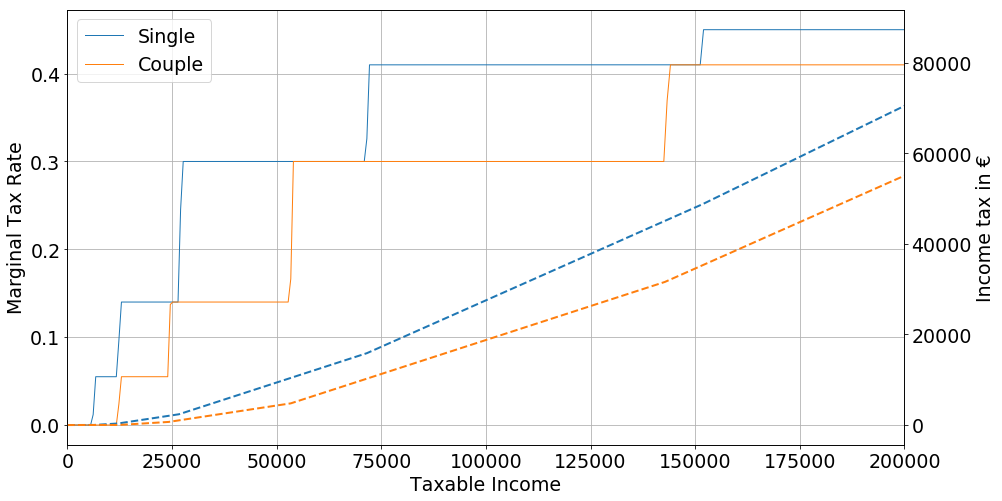
\includegraphics[width=1.2\textwidth]{MTR_for_single_and_couple.png}}%
    \label{fig:MTR_single_couple}
  \end{figure}
  Plain lines represent the marginal tax rate (left scale), I see that for the global income of the household, each tax bracket of the couple is twice the size of the single, including the zero (or exemption) tax bracket. Dashed lines (right scale) represent the income tax liability.
  The first tax bracket that has a MTR of 5.5\% starts at 5,963 \euro{}, while it starts at 11'926 \euro{} for married couples. The second tax bracket (14\% MTR) starts at 11'896 \euro{} for the single while it only starts at 23 792 \euro{} for the married couple.\footnote{$27792 = 5963*2+(1896-5963)*2$} The span of the first bracket is thus of 5'933 euros for a single,  11'866 \euro{} which is twice the single tax bracket span size.
  
  
\paragraph{Fiscal gain to children: } Following the previous reasoning, tax brackets of a couple with children will be larger than the one of a couple without child.\footnote{25\% larger for one child, 50\% for two, twice larger for three, and $\frac{n+1}{2}$ times larger for households with $n\geq 3$ children. This is just the result of the ratio $\frac{\text{Number of fiscal shares with children}}{\text{Number of fiscal share without children}}$.}
As the total income tax function is the integral of the MTR function, the fiscal gain to of n children is simply the area between the marginal tax rate of a couple and the marginal tax rate of a couple with n children.





%TODO: Add legend fot the black line

\begin{figure}[H]
  \caption{French income tax for a couple wiithout children, and a couple with one child}
\makebox[\textwidth][c]{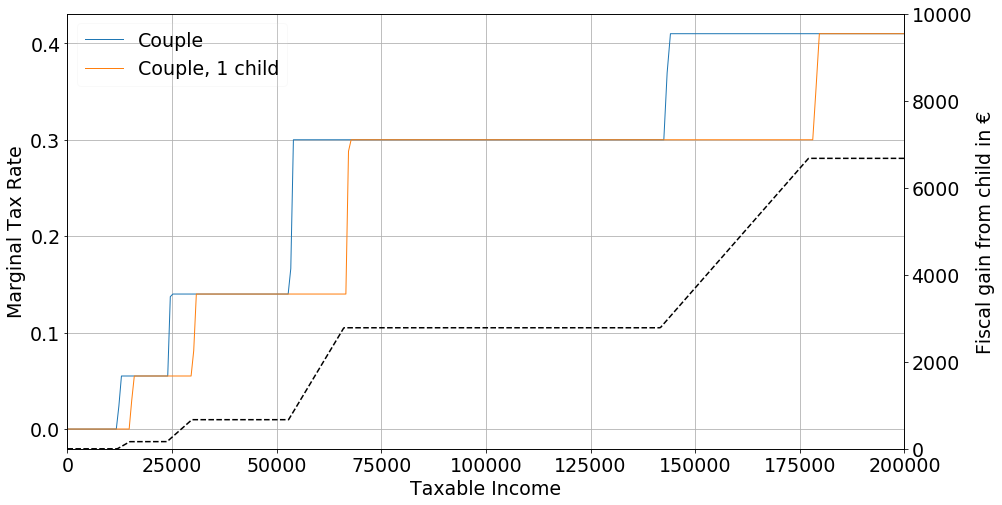
\includegraphics[width=1.2\textwidth]{MTR_for_couple_and_couple_1_child.png}}%
\label{fig:MTR_couple_couple_1_child}
\end{figure}

\autoref{fig:MTR_couple_couple_1_child} shows in plain line the MTR for a couple and a couple with one child. I see that each tax bracket is 1.25 times larger. The fiscal gain that is derived from the child is simply the area between the two MTR curves.\footnote{Or more specifically the difference between the integral of the couple MTR and the integral of the couple with n child integral}
The dashed line represents the fiscal gain due to the presence of a child in a fiscal household. I clearly see that the fiscal gain increases only when the two marginal tax rates are not the same, i.e. when the family ratio scheme put the household on a lower tax bracket.

\medskip

However as the children tax break can be very large as the number of children increases, the fiscal gain per half fiscal share is however bonded by a ceiling.
\medskip


\begin{figure}[H]
  \caption{French income tax with the tax child break ceiling }
  \label{fig:couple_couple_1_child_before_after}
\makebox[\textwidth][c]{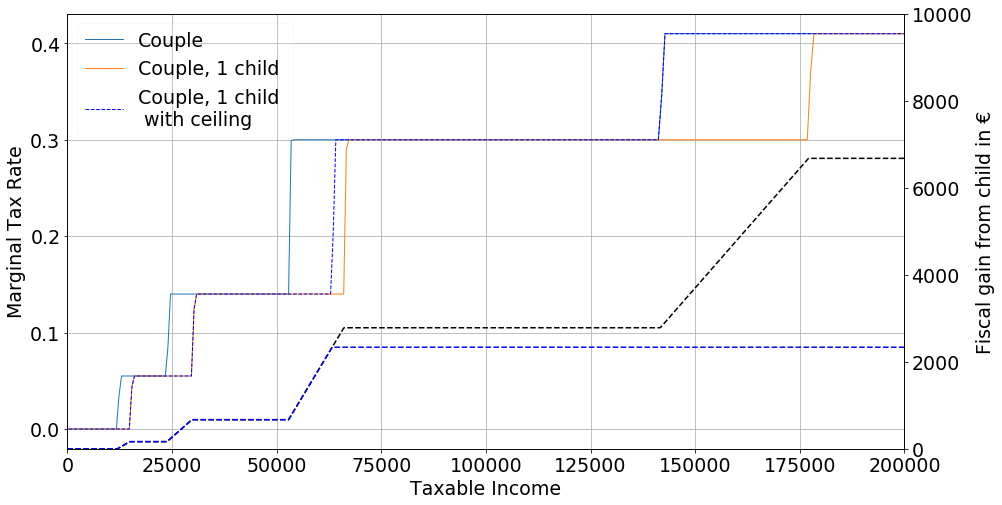
\includegraphics[width=1.2\textwidth]{MTR+Chil_fiscal_gain_1_child_3.png}}%
\end{figure}














This ceiling is a fixed amount per half fiscal share. That amount was of 2336 euros in 2011. 

During its presidential campaign that started in March 2011, François Hollande who was seen as very unlikely to win the presidential campaign did not make any announcement about a possible change in the children tax break associated with the family ratio scheme. He won the left-wing primary election in October 2011, and it is only in January 2012 that he released a set of 60 presidential propositions where he made an ambiguous claim about a change in the tax break related to children.
\footnote{ He stated "I'll leave unchanged all the resources allocated to the family policy. [...] I'll make more just the family ratio scheme by lowering its ceiling for richest households, which will concern less than 5\% of the fiscal-households"}
In May 2012 he won the presidential election against former president Nicolas Sarkozy with 51.62\% of the votes. It is only as late as in September 2012 that the reform of the threshold of the family ratio scheme has bee announced, then voted in December 2012.

The French income tax voted in December 2012 is applied to income earned during the year 2012 (the fiscal rules are thus known by the tax-payer after she has earned her income). As some anticipated behavior could have happened during 2012 about the lowering of the family ratio scheme reform, I claim that anticipation of the tax reform during the year 2011 is extremely unlikely: François Hollande was not seen as a potential winner of the presidential election before October 2011, the potential reform was not announced before 2012, and he only had a narrow victory.

\textbf{I thus take 2011 taxable income as the pre-reform period.} The reform consisted of lowering the family ratio scheme ceiling from 2336 euros to 2000 euros. A year after a new lowering of that threshold from 2000 to 1500 euros happened and was announced as a permanent reform. As the reform was announced in September 2013, to embody fully the effect of the reform I will take 2014 income as the post-reform year.

These two fiscal reforms have overall lowered the maximum child tax break ceiling from 2336 euros to 1500 euros, and in order to use a classical before and after the reform analysis, I will consider from now on that it constitutes a unique fiscal reform. 

  \begin{figure}[H]
      \caption{Income tax wich maximum child tax break before and after the reform}
      \label{fig:couple_couple_1_child_before_after_2}
    \makebox[\textwidth][c]{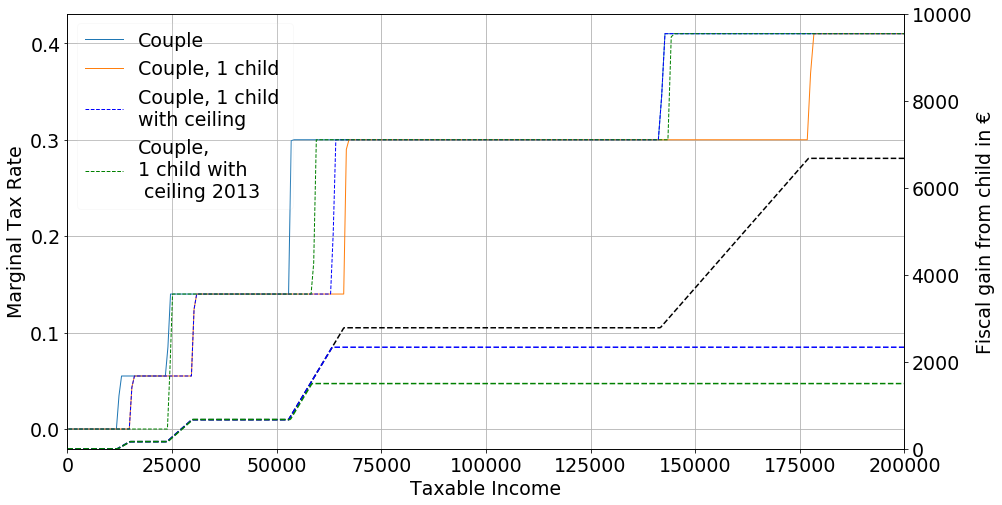
\includegraphics[width=1.2\textwidth]{MTR+Chil_fiscal_gain_1_child_4.png}}%
  \end{figure}



\autoref{fig:couple_couple_1_child_before_after_2} shows the ceiling before the reform, and after the reform: it limits the fiscal gain derived from children to 2336 euros in 2011 for couples earning more than 68 000 euros, and to 1500 euros in 2013 for couples earning more than 63 000 euros.  What is important here is to see that the impact of reaching the ceiling, is that a household jumps to the marginal tax rate it would have face without children (here the 30\% tax bracket).



The consequence is that there exists an income threshold at which the 2013 ceiling constraint is saturated and a threshold at which the 2011 ceiling constraint is saturated. This threshold is different for each family composition. 













\begin{figure}[H]
  \caption{Qf advantage from 1 to 5 children.}
  \label{fig:QF_from_1_to_5}
    \makebox[\textwidth][c]{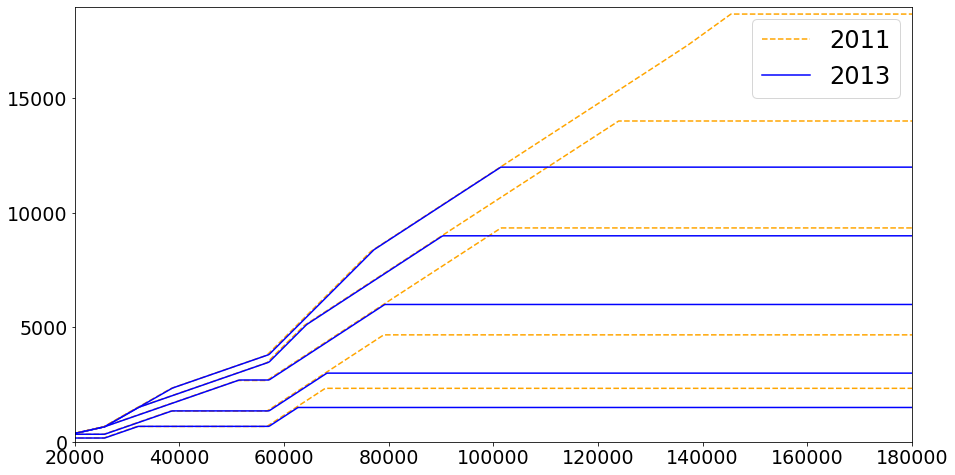
\includegraphics[width=1\textwidth]{fig_thresholds.png}}%
    \label{fig:key}
  \end{figure}
\medskip 

%TODO: bigger legend.
\autoref{fig:QF_from_1_to_5} shows the children fiscal gain for families from bottom to top of 1 to 5 children. 
Households have been affected in three ways. Households for which the fiscal advantage per child was lower than 1500 euros are unaffected. Households for which the fiscal advantage per child was between 1500 euros and 2336 euros (or twice that amount over 3 children) face a change in their marginal tax rate. 
Households for which the fiscal advantage per child was over 2336 euros faced a lump sum loss in disposable income of 836 \euro{} per child. The maximum fiscal loss that households can have are far from negligible since it represents up to 1.2\% of the disposable income of a family with one child, and respectively up to 2.2\%, 3.4\%, 4.1\%, 4.8\%, 5.4\% respectively for households from 2 to 6 children.
\footnote{see \autoref{fig:percent_loss} in appendix.}

As the fiscal advantage increases with income, there exists an income threshold at which a household will attain the ceiling. This thresholds is specific for each family composition, and since the ceiling has been lowered between 2011 and 2014, 

  \begin{table}[H]
  \caption{Income triggering FQ threshold based on taxable wage}
  \label{tab:thesholds}
  \centering
  \begin{tabular}{lrrrr}
  \toprule
  {Number of children} &                 2011 &                 2014  & Span & Maximum Fiscal Loss\\
  \midrule
  1 &         67,856  &         62,519               & 5,337 & 836  \\
  2 &         78,895  &         68,140                 &10,755 & 1672 \\
  3 &         101,426 &         79,166              &22,260 & 3344 \\
  4 &         123,756 &         90,221              &33,535 & 5016 \\
  5 &         145,188 &         101,272              &43,916 & 6688 \\
  6 &         159,477 &         112,324              &47,153 & 8360 \\
  \bottomrule
  \end{tabular}

  \end{table}

 
%  Reforms taking place in 2012, and 2013 has lowered this threshold from 2336 euros, to 2000 euros in 2012, and 1500 in 2013.
%
%
%  The threshold of the FQ concerns mostly last decile of income, the lowering implied loss in income at certain threshold, and change in marginal tax rates at others.






\autoref{tab:thesholds} shows the location of those thresholds in 2011 and 2014. Fiscal loss is computed by multiplying the number of fiscal shares by the difference between 2336 and 1500 \euro{}.

  For a given family composition, households being below their 2013 threshold are unaffected by the reform. Households being between 2013 and 2011 thresholds face a change in their marginal tax rate. Households being over 2011 thresholds face a lump sum decrease in their disposable income.




\medskip





%
%
% Interestingly (and surprisingly to us) I see that for a 1 and 2 children, 2013 thresholds are (nearly) the same as 2011 threshold s but with one less child. Indeed $\text{Threshold}_{2011}^{\text{1 child}} \approx \text{Threshold}_{2013}^{\text{2 child}}  $ This means that up to a lump sum transfer, the income tax would be the same for a household that switch from 1 child to 2 children between 2011 to 2013 (or from 2 children to 3).
%


One condition to evaluate correctly the impact of a reform is that it is not polluted by other reform taking place at the same time that concerns our population of interest. I am interested in the lowering of the family ratio scheme threshold, a first reform that could pollute our estimation are modifications in the piecewise linear tax scheme.

  \begin{table}[H]
  \center
  \caption{Piecewise linear tax scheme}
  \label{table:MTR}
  \begin{tabular}{lllrrrrll}
  \toprule
  {} & \multicolumn{2}{l}{2011} & \multicolumn{2}{l}{2012} & \multicolumn{2}{l}{2013} & \multicolumn{2}{l}{2014} \\
  {} &                 Rate &            Threshold &                 Rate &            Threshold &                 Rate &            Threshold &                 Rate &            Threshold \\
  \midrule
  0 &                    0 &                    0 &                    0 &                    0 &                    0 &                    0 &                    0 &                    0 \\
  1 &                0.055 &                5,963 &                0.055 &                5,963 &                0.055 &                6,011 &                 0.14 &                9,690 \\
  2 &                 0.14 &               11,896 &                 0.14 &               11,896 &                 0.14 &               11,991 &                  0.3 &               26,764 \\
  3 &                  0.3 &               26,420 &                  0.3 &               26,420 &                  0.3 &               26,631 &                 0.41 &               71,754 \\
  4 &                 0.41 &               70,830 &                 0.41 &               70,830 &                 0.41 &               71,397 &                 0.45 &              151,956 \\
  5 &                      &                      &                 0.45 &              150,000 &                 0.45 &              151,200 &                      &                      \\
  \bottomrule
  \end{tabular}

  \end{table}

\autoref{table:MTR} show the evolution of the marginal tax scheme over our period of interest. Two modifications have happened, the first one is the introduction of a new top tax bracket for single's tax-unit earning over 150 000 euros, and the second one is the suppression of the 5.5\% tax bracket.

The introduction of a 45\% tax bracket doesn't really concern our analysis because I focus on married couples earning from 50 to 200k\euro{}, their maximum equivalised taxable income will thus be 100k\euro{} and are thus too poor to be concerned by that reform. Thus suppression of the 5.5\% tax bracket has been concomitant to the decrease of the 14\% tax bracket threshold, the resulting total impact for households that have an equivalised income of 11'896 euros or greater is of 18 \euro{},\footnote{(11896-5963)*0.055 - (11896-9690)*0.14 } and represent a negligible amount of the disposable income of our concerned households (less than 0.01\%).

Many other small modifications have taken place during that period (such as very small inflation adjustments of the income tax brackets), but always account for less than 0.02\% of disposable income, and I thus choose to consider them as negligible.\footnote{ An interactive graph that displays that information that is accessible at the following link : \begin{sloppypar}\url{https://adrienpacifico.github.io/docs/bokeh_graph.html}\end{sloppypar} }

Another tax reform that could cause a potential bias is a change of tax base for capital income that happened in 2013.\footnote{The so called "fin du prélèvement forfétaire libératoire" reform.} Luckily I have a specific variable for the specific income that was concerned by that tax scheme.\footnote{ZIMPVALM in the database}
I ran the estimation with and without households that had income concerned by that specific tax regime in 2011, the results are all very similar and are provided in the appendix. 





Even if the number of tax bracket changes over time, I can see that the 30\% tax bracket starts, to the exception of small inflation adjustment, remains the same over the period. 
  The impact of the reform mainly concerns households that will switch from the 14\% tax bracket to the 30\% tax bracket or that already were on the 30\% and that faced a lump sum loss.

  
  
%  
%  
%  
% \footnote{Fran�ois Hollande has been elected in may 2012, the lowering of the family ratio scheme was very unclearly defined in its campaign program. Fran�ois hollande began his campaign at the end of March 2011 and general opinion was that he doesn't stand a chance of being elected. At that time Dominique Strauss-Kahn (DSK) was suspected by many observers to be the left-wing representant at the presidential election, but mid-may DSK has been accused of sexual assault and took him out of the presidential election. Then a primary election has been held which has been won by Fran�ois Hollande in October 2011. January the 26th Fran�ois Hollande realesed 60 political proposals into which figured the one that could be linked as a lowering of the family ratio scheme which stated "I'll left unchanged all the ressources allocated to the family policy. [...] I'll make more just the family ratio scheme by lowering its ceiling for richest households, which will concerns less than 5\% of the fiscal-households".
%  \footnote{\quote{Je maintiendrai toutes les ressources affect�es � la politique familiale. J'augmenterai de 25\% l'allocation de rentr�e scolaire d�s la prochaine rentr�e. Je rendrai le quotient familial plus juste en baissant le plafond pour les m�nages les plus ais�s, ce qui concernera moins de 5\% des foyers fiscaux.\\
%  Fran�ois Hollande, 60 engagements pour la France, p.15. 26/01/2012 }}
%  On the presidential election Fran�ois Hollande won against former president Nicolas Sarkory with 51.62\% of the votes.
%  In september 2012 the lowering from 2336 euros to 2000 euros has been annonced by the government. At the end of december 2012 the fiscal law has been voted with the first step of the lowering of the QF.
%
%
%  In France the income tax of year N is applied on income N-1
%  A behavioral reaction to the arrival of a potential reform in 2011 of the households seams unlikely since: i) If the reform has been foreseen by taxpayers, their incentive to react wasn't effective before January the first 2012, ii) the specificities and the second part (2013) of the reform wasn't planned at all.
%
%  The reform can thus be considered as an exogenous treatment that didn't had effect before 2012, that allows to consider is as a neat quasi-experiment.}
%end Section The reform



\section{Empirical Approach:}


To study the impact of the lowering of the maximum child tax break that happennend in 2012 and 2013 I use the \textbf{Echantillon Demographique Permanent} (EDP) the first release of which was in 1999 but that was enriched in March 2017 with new administrative data sources from which I use tax returns pieces of information and pay slips.
The database contains over 2.47 million households in 2014 and 2.38 million households for the year 2011.

I choose to focus my analysis on married couples and couples under civil union as it is the most standard family composition in France.
I thus select this population of interest and I am left with 1.19 million households and 1.16 million that I can observe in 2014 and 2011. There exist two forms of civil contract in France: civil partnership (PACS) and marriage. As there is no difference in the fiscal rules applied to married couples and couples under civil partnership, I will for a matter of convenience I  refer to them as married couples.



Singles represent a smaller share of the population and the tax reform implies different thresholds and effect than the one that applies on couples, although the same methodology as the one that I apply on married couples.


Cohabitants are also less common than couples under civil union, the analysis of the reform on those couples would be more complex as cohabitants can choose to allocate their fiscal shares on one of the two fiscal units that compose the household. Moreover, even if that complexity is taken into account, the limitation in the number of concerned households would probably be too small to derive any conclusion.
  
From those, I end with only 812 000 households present in both years in the database. The attrition of the 350000 households has many factors such as the death of the taxpayers, dissolution of marriage, change of address and so on.



\subsection{Data-Selection}
\paragraph{Income Span}
When it comes to identifying behavioral income reaction to a tax change, the biggest challenge is that the level of income tax is determined by the income itself and the two variables are thus endogenously linked.

I assume that belonging to a specific income span implies to be treated by the reform. As it is usual to instrument the counterfactual MTR in the literature by running a 2SLS estimation, this method, however, needs to have access to more than two years of data with multiple tax reforms over the period. 
%CONTINUE cite Saez, etc and Weber to justify this framework (Instrument income: not possible, 2 periods.). Only 2010 income are available 

As I want to analyze the impact of one tax reform I cannot do so.

There have been other tax reform that change the fiscal gain to children over the period, but none of them concerned households earning more than 50'000 euros. I then choose to limit the analysis to households earning less than 200'000 euros per year. First for those households well over the last percentile of the income, distribution the number of observations is small, second they are more likely to be able to do income shifting through many channels, third they are less impacted by the reform since for most households the impact of the reform is maximum for households earning less than 100'000 euros. 

As emphasized by \citet{kopczuk2005tax}, estimations are very sensitive to data-selection and data-trimming. As the estimation does not fully concerns the very end of the income distribution I am not upward bounded by the richest household of the distribution. 

What I do is to select households that its taxable income located between 50'000 euros and 200'000 euros either in 2011 or in 2014.
\footnote{To be fairly explicit a household earning 40k\euro{} in 2011, and 55k\euro{} in 2014 will be in the sample. A household earning 170k\euro{} in 2011, and 220k\euro{}  in 2014 will be in the sample, a household earning 30k\euro{} in 2011 and 45 k\euro{} in 2014 will not be in the sample.}
 By doing so I avoid the mean reversion bias. 
Indeed since I control for the position in the income distribution, differences in trends between high-income earners and low-income earners will be captured which will cancel out the change in distribution bias.
By selecting households that were in the 50-200k euros range in either 2011 or 2014 I claim that I control for the remaining mean reversion. Indeed if households face reversion of the mean, by selecting households that were earning between 50-200k euros in 2011 or in 2014, since mean reversion is defined as mean zero shock at each period, if an household face an income shock unrelated to the tax reform that lead it to goes from 150'000 euros to 300'000 euros, it is euqually likely that an other household has an unrelated to the tax reform shock from 300'000 euros to 150'000 euros one I controlled for the position in the income distribution. Thus the effect of mean reversion will be canceled out.

If I selected households that were on the 50-200k income span only in 2011, households that have transitory shock that leads them to be above the 200k threshold will not be compensated by those who were earning more than 200k euros in 2011 but that has negative transitory income shock. This would lead to overestimating the impact of being over the 2011 maximum child tax break threshold.

The same reasoning can be applied to households that leave the 50-200k income span for an income lower than 50k euros. To one exception, taxable income is bounded and cannot be lower than 0. This would be a problem as it is not clear that households whose earning falls to zero would be canceled out by households that have income that goes from zero to income in the 50-200k range. To cancels out this problem, I trim the sample based on change in earnings such that no households get a null income in the sample. This leaves out 4\% of the sample (2\% at the top and 2\% at the bottom). 



% \begin{enumerate}
%   \item not upward bounded (problem for mean reversion)
%   \item Does not apply to only a specific part of the income distribution, thus control for the change in distribution bias.
% \end{enumerate}

% \begin{enumerate}
%   \item If selection earning between 50-200k in 2011:\\
%         Would imply a selection bias: households that increase a lot their income will bias the sample, while 
%   \item If selection earning between 50-200k in 2014:
% \end{enumerate}


% \begin{enumerate}
%   \item If selection earning between 50-200k in 2011 and in 2014:\\
%         Would be polluted by mean reversion bias and outliers from events that are not linked with the tax reform.
%   \item If selection earning between 50-200k in 2014:
% \end{enumerate}

  
%  I then select married couples for that have the same number of children in 2011 and 2014.  I then select couples for which earnings belong to the 50-200k \euro{} either in 2011 or 2014. I do so to do not bias the estimate with possible mean reversion effect. 

\medskip





I then take the taxable income present in the database at the tax-unit level and sum them to obtain taxable income.

For now on I will consider that the effect of the reform corresponds to a specific treatment. Households that did not face a change in their income tax are untreated. Households for which the two thresholds are treated with Treatment 1, and the treatment is a change in MTR. And households that are over the 2011 threshold are treated with Treatment 2, and they face a lump sum loss in their disposable income.
  
  The repartition of households in those three groups is reported in \autoref{tab:number_of_concerned_households}.


  \begin{table}[H] %QF an evaluation of the income effect full
    \caption{Number of concerned households}
  \label{tab:number_of_concerned_households}
\centering
\begin{tabular}{l|rrr|l|}
\toprule
   {Number of children} &                 Treatment 0 &                 Treatment 1  & Treatment 2 & Total\\
\midrule
0 &     43960      &     0    &         0       &      43960            \\
1 &     16110      & 3324       &  11638          &   31072             \\
2 &     49720      & 11142    &     20033       &      80895            \\
3 &     21930      & 4747       &  5084          &   31761             \\
4 &     3571      & 774         &  651            &    4996             \\
5 &     578        & 113         &  42            &    733              \\
6 &     159        & 18         &  5              &    182              \\

\hdrule
Total & 136028      &  20118     & 37453          &   193599        \\
\bottomrule
\end{tabular}

\end{table} 


          
         
          
         
         
        
         
              






I see that the non-treated represents 193599 households which represent 56\% of the sample. Households facing a change in MTR represent 20118 households (14\% of the sample), and households that face a lump sum change represents 37453 households (28\% of the sample). I see that the number of households 6 children in the first treatment is of 18 households and only 4  in the second treatment. Such small numbers would likely leads the estimates to be driven by outliers or be subject to micronumerosity/partial colinearity and should be taken with caution.  Although all the regression has been run with an iteratively reweighted least squares estimations to control for the impact of potential outliers and leads to very similar results



  % 
  % 
  % 
  % \section{Mechanical, and behavioural effect}
  % 
  % 
  % 
  %The reform is the sum of two separated effects on the total tax amount:
  %\footnote{A third element could be added which is a structural change in the society such as change in the number of children in the households, retirements, etc.}
  %
  %\begin{enumerate}
  %\item A mechanical one. It corresponds to the change in the tax amount due solely to the change of tax scheme. Namely $G_{2015}(y_{2011}) - G_{2011}(y_{2011})$ where $G_t$ is the tax scheme at time t, and $y_t$ is the tax scheme at time t.
  %\item A behavioural one. It correspond to the change in the tax amount due to the change of reported income due to change of tax scheme. Formally $G_{2015}(y_{2015}) - G(y_{2011})$ 
  %\end{enumerate}
  % 
  
  
  
  
\subsection{Tax base and tax computation}
The database contains pieces of information at the fiscal household level and at the individual level.
\footnote{When aggregated individual income match households income, with some exceptions due to tax deductions that are sadly not documented by the data producer (one example is for  rented furnished flat: individual income is twice the household income due to a 50\% tax rebate on flat rented furnished that is taken into account at the household level but not on the individual level. ). }
To compute the tax base I use a simple rule of thumb: I sum the 7 categories of income present in the database at the household level. I, however, apply the 10\% deduction for professional expenses on labor and retirement income.
\footnote{The 10\% tax deduction is computed by taking into account the different thresholds that can lead to a taxable income reduction greater or smaller than 10\%. I took formulas from the OpenFisca microsimulation software}
\footnote{However taxpayers can choose to deduce their real expenses to reduce their labor income tax base. Although it was a major concern to me that this may lead to overestimating the tax base, I provide evidence in the appendix that the impact is likely to be minor.} 

Once the tax base determines, I compute the tax liability by applying OpenFisca income tax formulas.
 



%end section Data
\subsection{Descriptive Statistics}
The set of administrative databases and administrative surveys provide a very rich set of variables. Those variables do not always cover fully the population. A set of descriptive statistics for each treatment group are reported in \autoref{descriptive statistics}.

\renewcommand{\arraystretch}{0.8}
\begin{table}
    \caption{Summary statistics}
    \label{descriptive statistics}
    \centering
    \resizebox{\columnwidth}{!}{%
      \begin{tabular}{lcccccccccccc}
      \toprule 
    & \multicolumn{1}{c}{All}
    & \multicolumn{1}{c}{Treatment 0}
    & \multicolumn{1}{c}{Treatment 1}
    & \multicolumn{1}{c}{Treatment 2}
     \\ %\cmidrule{2-4}  \cmidrule(lr){5-7} \cmidrule(lr){8-10} \cmidrule(lr){11-13} \\
    \cmidrule(lr){2-2}  \cmidrule(lr){3-3}  \cmidrule(lr){4-4}  \cmidrule(lr){5-5}  
    
     
    
    Taxable income                          &    66018            & 55611       &71816                                  	      	&100704	                \\       
    $\Delta$ Taxable income	                &   6222            	& 6647     	 	&5305                                   	       	&5174	                \\   
    \midrule    
    Father is working 2011	                &   0.866             	& 0.840	    &0.932                               	          	&0.9260                 \\        
    Mother is working 2011	                &   0.766             	& 0.759	     &0.809                               	          	&0.7689                 \\        
    Father is employed 2011                 &	 0.823            	& 0.809	     	&0.886                               	          	&0.8408                 \\        
    Mother is employed 2011                 &	 0.775            	& 0.767	     	&0.820                               	          	&0.7812                 \\        
    Father is employed 2014                 &	 0.732            	& 0.709	     	&0.815                               	          	&0.7707                 \\        
    Mother is employed 2014                 &	 0.709            	& 0.696	     	&0.768                               	          	&0.7215                 \\  
    \midrule      
    Mother's salary 2011	                  &   37389           	& 30812     	&44103                                  	      	&57667	                \\       
    $\Delta$ Mother's salary	              &  224              	&  161    	 	&650                                	          	&226                    \\     
    Father's salary 2011	                  &   22251           	& 19676     	&24706                                  	      	&30281	                \\       
    $\Delta$ Father's salary	              &  -761             	& -724    	 	&-137                                   	      	&-1230	                \\       
    $\Delta$ Retirement income_wo	          & 665               	& 877     	 	&104                                	          	&196                    \\         
    $\Delta$ Retirement income_me	          & 1411              	& 1780     	 	&303                                	          	&663                    \\         
    $\Delta$ sel-employed income_wo	    & 13                	& 199   	  	&140                                	          	&-97                    \\         
    $\Delta$ sel-employed income_me	    & -1                	& -15   	  	&-3                                 	          	&-533                    \\
    \midrule             
    Father independant worker 2011	        &   0.054           	& 0.040	     	&0.064                               	          	&0.0973                 \\        
    Mother independant worker 2011	        &   0.084           	& 0.068	     	&0.086                               	          	&0.1439                 \\        
    \midrule
    Mother is retired 2011	                &   0.042             & 0.056	     	&0.008                               	          	&0.0111                 \\        
    Mother retired 	                        &  0.029             	& 0.039	     	&0.005                               	          	&0.0084                 \\        
    Father is retired 2011	                &   0.049             & 0.067	     	&0.006                               	          	&0.0082                 \\        
    Father retired 	                        &  0.044             	& 0.056	     	&0.012                               	          	&0.0190                 \\        
    \midrule         
    Father start working	                  &    0.020          	& 0.022	     	&0.016                               	          	&0.0143                 \\        
    Mother start working	                  &    0.009          	& 0.011	     	&0.004                               	          	&0.0050                 \\ 
    \midrule        
    Mother stop working ($\neg$retired)	    & 0.064             	& 0.062	     	&0.067                               	          	&0.0689                 \\        
    Father stop working ($\neg$retired)	    & 0.064             	& 0.063	     	&0.068                               	          	&0.0666                 \\  
    \midrule       
    Centile 2011 (std of living)	          &    81.10          	& 76.746     	&86.801                              	          	&93.86               \\         
    Centile 2014	(std of living)           &    81.37          	& 78.222     	&83.612                              	          	&91.63               \\  
    \midrule       
    Income tax 2014	(administrative)        &   6797            	& 4700    	 	&6402                                   	      	&14624	                \\       
    Income tax 2011 (administrative)        &   4996              & 3492    	 	&3776                                   	      	&11114	                \\       
    Income tax 2014 (author's computation)  &   8486            	& 5896    	 	&8378                                   	      	&17952	                \\       
    Income tax 2011 (author's computation)  &   6769            	& 4768    	 	&5701                                   	      	&14608	                \\
    \midrule       
    Computed MTR from 
     administrativeIncome tax &   0.206   	& 0.171	     	&0.270                               	          	&0.299                  \\      
    Computed MTR 2011	                      &   0.192           	& 0.167	     	&0.140                               	          	&0.311                  \\      
    Computed MTR 2014                       &   0.231           	& 0.204	     	&0.271                               	          	&0.308                  \\ 
    \midrule     
    Share 0 child                           & 0.227              	& 0.323	     	&0.000                               	          	&0.000                  \\      
    Share 1 child                           & 0.160              	& 0.118	     	&0.165                               	          	&0.310                  \\      
    Share 2 children                        & 0.417              	& 0.365	     	&0.553                               	          	&0.534                  \\      
    Share 3 children                        & 0.164              	& 0.161	     	&0.235                               	          	&0.135                  \\      
    Share 4 children                        & 0.025              	& 0.026	     	&0.038                               	          	&0.017                  \\      
    Share 5 children                        & 0.003              	& 0.004	     	&0.005                               	          	&0.001                  \\ 
    \midrule     
    Age Father                              & 45.717            	& 46.102	   	&43.747                              	          	&45.37                  \\      
    Age Mother                              & 43.870            	& 44.360	   	&41.792                              	          	&43.20                  \\      
    Age Eldest Child	                      & 8.846              	& 7.847	     	&11.803                              	          	&10.88                  \\      
    Age Youngest child	                    & 6.755             	& 5.825	     	&9.030                               	          	&8.91                   \\  
    \bottomrule    
    \end{tabular}%
    }
\end{table}
    
\renewcommand{\arraystretch}{1}



\paragraph{Marginal Tax Rates: } The tax reform implied a change in marginal tax rates for households that are between the 2011 and 2014 thresholds.







\begin{figure}[H]
    \caption{MTR before and after the reform}
    \label{fig:MTR-2011-2014}
  \makebox[\textwidth][c]{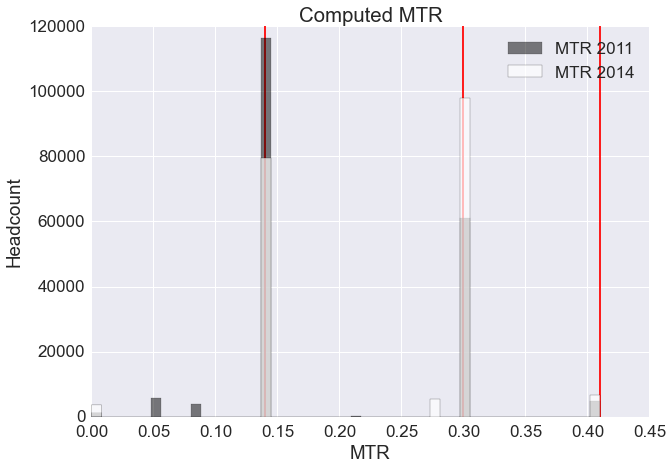
\includegraphics[width=0.7\textwidth]{/fig_casd/MTR_2011_vs_2014.png}}%
  %\label{fig:MTR_single_couple}
\end{figure}




		\begin{table}[H]
    \caption{Effective statutory rates before and after the reform.}
    \label{table:MTR-2011-2014}
    \center
    \begin{tabular}{@{}lllrr@{}}
    \toprule
& \multicolumn{2}{c}{Effective} & \multicolumn{1}{l}{Counterfactual:}\\
&               &               & 2011 tax on 2014 income\\
\cmidrule(lr){2-3} \cmidrule(lr){4-4}
MTR      & 2011   &  2014 & 2014 \\ 
\midrule      
0	  \%  & 00.65  &	01.88 &  0.00     \\
5.5 \%	& 03.03  &	00.00 &  0.84     \\
8.25\%	& 02.06  &	00.00 &  0.69     \\
14	\%  & 60.12  &	41.12 &  55.40     \\
21	\%  & 00.05  &	00.00 &  0.05     \\
28	\%  & 00.00  &	02.89 &  0.00     \\
30	\%  & 31.47  &	50.60 &  38.63     \\
41	\%  & 02.54  &	03.45 &  3.65     \\
\bottomrule
    \end{tabular}
    \end{table}
\autoref{table:MTR-2011-2014} and \autoref{fig:MTR-2011-2014} shows the MTR households were subject to in 2011 and 2014.
\footnote{I computed those rates by taking the taxable income for a given year }
If I ignore the changes due to the suppression of the first tax bracket and the implicit tax brackets created by the decote mechanism,
\footnote{which multiplied the statutory rate for households concerned by the mechanism by 1.5 in 2011 and 2 in 2014. That creates the 8.25 and 21\% implicit marginal tax rate for 2011 and the 28\% implicit MTR for 2014 (e.g  for the 5.5\% tax bracket $5.5\% \times 1.5 = 8.25$) } 
I see that the main change in the repartition of households in the income tax scheme is a change from the 14\% tax bracket (from 60\% to 41\% of the sample) to the 30\% tax bracket (from 31\% to 51\% of the sample). 

The fact that households shifted from the 14\% MTR to the 30\% MTR can be due to two distinct causes. The first one is due to the fact that income has increased over the period. The other one is due to the lowering of the family ratio scheme. To disentangle those the two, I can look at the 2014 counterfactual income tax, which is the income tax a household would have paid if the 2011 income tax schedule would have been applied to its 2014 income. I see that the 19\% decrease in households being on the first tax bracket, 5\% can be attributed to the general increase in income in the population, and thus 14\% is due to the lowering of the family ratio scheme.


% \paragraph{Population by treatment:}
% \begin{table}[H]
%     \caption{Change in taxable income on income location}
%     \label{table:Treatement_location_by_child_or_not}
%     \centering
%     \resizebox{\columnwidth}{!}{%
%     \begin{tabular}{llllllllllllllll}
%     \toprule
									
% 	 &         &    B1	 &   B2	 &    B3	&   B4	 &     B5	 &   O1	 & O2	 & O3	&  O4	& O5                \\ 
% \midrule 
% \multirow{ 7}{*}{All}
% &   All	        &  3312	 & 3588	 &  3906	& 4168	 &   4567	 & 3958	    & 4200 & 	4561	&  4570	 &4536                \\ 
% &   Treatment 0	&  3288	 & 2173	 &  -775	& -2246  &  	-2145	 & 657	  &-1168 & 	-1877 & 	-1574	 &-989                \\ 
% &   Treatment 1	&  3433	 & 4964	 &  7125	& 7254	 &   6702	 & 5676	    &7078  &	6671	&  1054	 &1670                \\ 
% &   Treatment 2	&   --	 & 3363	 &  4705	& 5526	 &   6164	 & 5174	    &5427  &	6049	&  5988	 &5718                \\ 
% \cline{2-12}
% &   Children	  &  4522	 & 4931	 &  5392	& 5822	 &   6199	 & 5423	    &5704  &	6077	&  5940	 &5714                \\ 
% &   No child	  &  -421	 & -1172 & -1696	& -2451  &  -2213  &-1544     &	-1803 & 	-1928	 &-1574&	-989                \\ 
% \midrule
% &   Non Treated	&  4828	 & 6216	 &  7784	& 8157	 &  22311  & 6219     &	7574	&  22311	 &--	 &--                \\ 
% \multirow{ 3}{*}{With children}
% &   Treated	    &  3433	 & 4515	 &  5322	& 5810	 &   6188	 & 5330	    & 5669 & 	6069	&  5940	 &5714                \\ 
% &   Treatment 1	&  3433	 & 4964	 &  7125	& 7254	 &   6702	 & 5676	    & 7078 & 	6671	&  1054	 &1670                \\ 
% &   Treatment 2	&   --	 & 3363	 &  4705	& 5526	 &   6164	 & 5174	    & 5427 & 	6049	&  5968	 &5718                \\ 
% \bottomrule
% \end{tabular}%
% }
% \end{table}
% %TODO add a line to state the income location of B1, B2, B3, etc.



\subsection{Identification Strategy}



  % I am going to estimate the effect of the reform by using a triple difference framework with two treatments per each family type (per children number), and many control groups which has a complex structure based on a non-overlap of treatments with respect to each group. As the French income tax 


  % Our estimation makes, however, some assumption, the first one is that I correctly described the reform and that the tax-base is correctly observed in the database. One concern is that I do not have the information about professional expenses that are to some extent tax deductible which would lead us to overestimate the tax base. However the database contains the income tax that households actually paid, in \autoref{how_precise} I compare the expected change in tax and expected marginal tax rate, I show that (even if not perfect) the estimates are consistent with a pretty accurate description of the reform.


  % In order to fit our problem in the classical public policy evaluation literature I am going to start from a simple diff-in-diff problem, then increase the complexity of the estimation towards our preferred regression.



\paragraph{A difference-in-difference} is based on the estimates of the dependent variable based on the interaction of two binary variables: the after reform one and the treated group one. An after reform binary is also included in the regression to account for the mean evolution of the dependent variable between,  before and after the reform. The treated binary is also included to account for the possible difference between the treated and the control group prior to the policy change.
  \begin{equation}
  y_{it} = \beta_0 + \beta_1 \text{Post}  + \beta_2 \text{Treated}  +  \delta  \text{Treated} \times \text{Post}  + c_i + \epsilon_{it}
  \end{equation}

  When using individual-level panel data $c_i$, the individual fixed effect is included to control for individual unobserved effect.\\
  The OLS estimate of $\hat{\delta}$ implies : 
  $\hat{\delta} = \Delta \bar{y_{\text{treated}}} - \Delta \bar{y_{\text{untreated}}} $,

  which represent the dependent mean evolution of the treated group minus the one of the untreated group, which is stated as the effect of the treatment.

  This equation can be evaluated through a first difference setting which leads to : 

  \begin{equation}
  \Delta y_{i} =   \beta^{'}_1+ \delta_1^{'}  \text{Treated} + \epsilon^{'}_{i}
  \end{equation}

  And I have $\delta_1^' = \delta_1$, and $\beta^'_1 = \beta_1$.


  \paragraph{Back to our case,} I have a change in the tax scheme happening between 2012 and 2013. 
  This change in tax scheme gives three groups: the control group, the group facing the first treatment (i.e. being between the 2011 and 2013 thresholds), and the one facing the second treatment (i.e. being over the 2011 threshold).
  I can thus run a difference in difference regression with two treatments.

  \begin{equation}
  \label{eq:DD_simple}
  \Delta y_{i} =   \beta_0+ \delta_1 \text{Treatment}_1 + \delta_1 \text{Treatment}_2  + \epsilon_{i}
  \end{equation}

  $\delta_1$  account for being between the two brackets,  a negative sign would imply that the substitution effect due to the increase of the leisure price dominates the income effect, a positive sign would imply that the income effect dominates. $\delta_2$ represent the effect of being above the 2013 bracket since it implies a reduction in disposable income without a change in the marginal tax rate, I would expect a positive sign.

Some assumptions are conditional for $\delta_1$ and $\delta_2$ to capture the refom. 

One key assumption is that the counterfactual without the reform would imply that the taxpayers would still have its income in the treatment span.



  Such a regression doesn't take into account the position in the income distribution. It is possible that being on a specific position of the income distribution the variation of income will have a different trend and that this trend concerns more specifically the treated. It is also possible that the variation of income depends on the number of children in the household and that the parameters capture mainly a big part of the difference between the mean evolution of households with children against households without children.
  I thus run the regression by including control variables for the number of children, and a binary is added for the effect of being over the 2011 thresholds (from 1 to 6 children).



 This leads to a  Difference-in-Differences-in-Differences estimation that allows to control for potentially confounding trends: change in income due to the position in the distribution, the number of children in the household, and possible interactions between the two. Such a property of the French family ratio scheme is quite remarkable and has indeed been emphasized by \citet{piketty1999hauts}.
 
 
 
  This regression also considers Treatment 1 and Treatment 2 as different treatments for each number of children in the household, which allows to see the specific impact of the reform for a given number of children. The result is the following estimator, which is formally a triple-difference estimator with 12 treatments.




  \begin{align}
    \label{eq:triple-diff}
  \begin{split} 
  \Delta y_i &= \beta_0 + \sum_{i=1}^{6} {\beta_i \text{Children}_i} + \sum_{j=1}^{6} {\prescript{}{b}\delta_j \text{Between}_j}  + \sum_{j=1}^{6} {\prescript{}{o}\delta_j \text{Over}_j} \\
      &+ \sum_{i=1}^6 {\prescript{}{b}\gamma_{i} \text{Children}_i \times \text{Between}_i} \\
      &+ \sum_{i=1}^6 {\prescript{}{o}\gamma_{i} \text{Children}_i \times \text{Over}_i} \\
      & + \epsilon_i
  \end{split}
  \end{align}




$\Delta y_i$ represent the change in taxable income between 2011 (before the reform) and 2014 (after the reform).

  The intersect $\beta_0$ captures the time trend, i.e., the mean change in wage between 2011 and 2014. $\text{Children}_i$ is a dummy indicating for the number of children (the reference being 0 children), $\beta_i$ thus captures the variation in income for i children in the household. \\ $\delta $  capture the effect of being on a specific part of the distribution: $\prescript{}{b}\delta_i $ captures the effect of being on the position in the distribution where the treatment 1 applies to households having 1 child. $\prescript{}{o}\delta_i $ captures the effect of being above the 2011 threshold for a given number of children i.


  The parameters of interest are $\prescript{}{}\gamma_i $, i.e., the triple difference estimators. Those are the parameters that capture the interaction between being on the specific location of the income distribution, where for a given number of children in the household the treatment took place, interacted with that given number of children. The left subscripts b, and o, account for respectively the first treatment  (between thresholds), and the second treatment (over 2011 threshold).
  

  The first parameters of interest $\prescript{}{b}\gamma_i $, captures the effect of the change in marginal tax rate (MTR).  The sign of the parameter determines whether the income effect dominates, or the substitution effect dominates. If the sign is positive, the income effect dominates (the loss in income due to the reform implied an increase in the effort to compensate for the loss in income). It the sign is negative, the substitution effect dominates: the increase in MTR leads to favor leisure over income.


Such estimation makes it hard to determine what is the control group. The control groups is constituted first of households without children. Then it is also constituted by households with children that are below the 2013 ceiling. More surprisingly treated households also constitute a control group, but deflated of the mean estimated effect of the reform. This is because the estimate of interest (all the $\gamma$) capture the mean effect of being in the treatment group.\footnote{This fact has been checked with numerical simulations. }






For example the OLS estimate $\hat{\prescript{}{b}\gamma_3} $, accounts for the effect of the 2012/2013 reform on the household with three children for which income was between 79 166 euros and 101 426 euros can be expressed as follow : 

\begin{align}
\begin{split}
\hat{\prescript{}{b}\gamma_3}  &= \left( \bar{y}_{T^1_{3, 3C, 2014}} - \bar{y}_{T^1_{3, 3C, 2011}} \right) \\
&- \left( \bar{y}_{T^1_{3, \{0,1,2,4,5,6 \}C, 2014}} - \bar{y}_{T^1_{3, \{0,1,2,4,5,6 \}C, 2011}} \right) \\
& - \left( \bar{y}_{\neg T^1_{3, 3C, 2014}} - \bar{y}_{\neg T^1_{3, 3C, 2011}} \right) 
\end{split}
\end{align}

The first line of the left-hand side represents the mean change in income for the households of three children being between the 2014 and 2011 thresholds.

The second line represents the mean change in income for the households for which the number of children is not 3, but being between the 2014 and 2011 thresholds.

The third line represents the mean change in income for the households for which the number of children is 3, but not being between the 2014 and 2011 thresholds. I have thus controlled for two kinds of potentially confounding trends.

\paragraph{Flatten Thresholds:}
The series of thresholds $ \sum_{i=1}^6 {\prescript{}{b}\gamma_{i} \text{Children}_i \times \text{Between}_i}$,\\
     and $\sum_{i=1}^6 {\prescript{}{o}\gamma_{i} \text{Children}_i \times \text{Over}_i}$ are overlapping. For instance, as shown in \autoref{tab:thesholds},  a household with a taxable income of \mbox{95 000} euros, dummies will be true for $\text{Over}_1$ and $\text{Over}_2$ since the taxable income is greater than the 2011 threshold for 1 and 2 children. For that same exemple, the dummies $\text{Between}_3$ and $\text{Between}_4$ will also be true. 
    One consequence is that it is difficult to interpret the parameters linked with the dummies $Over_i$ and $Between_i$. However, each possible configuration of these dummies variables is a linear combination of all thresholds intervals once they have been ordered. The result is (for 6 children), 11 income span plus a twelve one for households over the highest threshold. \\x

    By substituting   $ \sum_{i=1}^6 {\prescript{}{b}\gamma_{i} \text{Children}_i \times \text{Between}_i} + \sum_{i=1}^6 {\prescript{}{o}\gamma_{i}\text{Children}_i \times \text{Over}_i} $ 
    in \autoref{eq:triple-diff} with  

    $ \sum_{i=1}^{12} \text{Income\_Span}_i $ the regression is strictly equivalent for all other parameters while allowing to have a clearly interpretable effect of being on a specific position in the income distribution. This is the way the results will be reported.


\section{Results: }



In order that tables keep a reasonable size, standard errors or parameters may be taken out when they are not crucial for the analysis.  Although all the results in that section are available at \url{https://github.com/adrienpacifico/fq_lowering/} with all parameters and standart errors, and with the exact code used to produce the results.






\paragraph{Triple Diff:}
I run the triple-diff estimation in three different manners. First, I run a classical ordinary least square (OLS) estimation that captures the average change in taxable income between 2011 and 2014. However, because I can expect that richer households would be more prone to --in absolute values-- larger income variations compare to poorer households,  the estimation is likely to be subject to heteroscedasticity. 

% Moreover by the way I selected our sample, the income variation is not bounded and  outliers can influence \footnote{Remember that the condition to be in the sample is to be in the 50-200 K\euro{} either in 2011 or 2014, it is thus possible that a households rise from 50k\euro{} to 1M\euro{}, or goes from 150k \euro{} to a very small income in cases of extreme events (e.g. job-loss)} the estimates. The estimation through a robust linear model with the iteratively reweighted least squares (IRLS) solves both issues.\footnote{See \citep{green1984iteratively}.} 


The literature on tax elasticity of entire population has focused on young working-age population and considers that older population de-facto less elastic \citep{alpert2013estimating, messacar2017incidence}, younger workers were more prone to changes and has broader prospects to make their income vary. 
%It seems to us sound to consider that younger individual should be more elastic than older individuals, reasons such as life-cycle hypothesis (i.e. 

\medskip

I propose two estimates: an OLS on all the population, an OLS with the age of the oldest parent as control.
%, one regression on a young household where the oldest parent is less than 50 years old, and one on old households where the oldest parent is over 50 years old. %\footnote{I chose the age of the men because
%TODO :  add HC3 to the OLS estimate



\afterpage{
\begin{table}[H]
\caption{Triple-diff estimate}
\label{table:Triple_diff_estimates}

\center
\adjustbox{max height=\dimexpr\textheight-4.5cm\relax,
           max width=11cm}{
\begin{tabular}{lcccc}
\toprule

                            &Triple                        & Triple age controls                      \\
\cmidrule(lr){2-2}  \cmidrule(lr){3-3} \\
$Over_{1} \times Child_1$	                     &$ 2292^{***} $                  & $ 2446^{***}$       \\
                                                 &$ (232)      $                     & $ (231)  $     \\
$Over_{2} \times Child_2$	                     &$ 4314^{***} $                  & $ 4363^{***}$       \\
                                                 &$ (237)      $                     & $ (236)  $     \\
$Over_{3} \times Child_3$	                     &$ 3996^{***} $                  & $ 3925^{***}$       \\
                                                 &$ (399)      $                     & $ (398)  $     \\
$Over_{4} \times Child_4$                        &$ 3120^{***} $                  & $ 3032^{***}$     \\
                                                 &$ (1054)     $                     & $ (1052) $     \\
$Over_{5} \times Child_5$	                     &$ 5174       $                  & $ 4846   $          \\
                                                 &$ (3955)     $                     & $ (3961) $     \\
$Over_{6} \times Child_6$	                     &$ -198       $                  & $ -727   $          \\
                                                 &$ (13784)    $                     & $ (13843)$     \\
\midrule                                                                                              \\
$Between1 \times Child_1$	                     &$ 621^{**}  $                   & $ 622**  $          \\
                                                 &$ (255)     $                      & $ (254)  $     \\
$Between2 \times Child_2$	                     &$ 2487^{***}$                      & $ 2496^{***}$    \\
                                                 &$ (197)     $                      & $ (197)  $     \\
$Between3 \times Child_3$	                     &$ 4234^{***}$                      & $ 4224^{***}$    \\
                                                 &$ (316)     $                      & $ (315)  $     \\
$Between4 \times Child_4$                        &$ 2780^{***}$                      & $ 2706^{***}$  \\
                                                 &$ (754)     $                      & $ (752)  $     \\
$Between5 \times Child_5$	                     &$ -4147^{*} $                      & $ -4254* $       \\
                                                 &$ (2194)    $                      & $ (2190) $     \\
$Between6 \times Child_6$	                     &$ -9431^{**}$                      & $ -9655^{**}$    \\
                                                 &$ (4765)    $                      & $ (4834) $     \\
\midrule  
$Child_1$                                        &  $1829^{***}$                  &372$^{***}$        \\
$Child_2$                                        &  $2662^{***}$                  &507$^{***}$        \\
$Child_3$                                        &  $4388^{***}$                  &2327$^{***}$       \\
$Child_4$                                        &  $6234^{***}$                  &4269$^{***}$       \\
$Child_5$                                        &  $7406^{***}$                  &5585$^{***}$       \\
$Child_6$                                        &  $8987^{***}$                  &7066$^{***}$       \\
\midrule                                                                                              \\
Taxable income $\in$ $[58291,63233]$             &   -5399$^{***}$                &-5186$^{***}$      \\
Taxable income $\in$ $[63233,63530]$             &   -5806$^{***}$                &-5600$^{***}$      \\
Taxable income $\in$ $[63530,73516]$             &   -6564$^{***}$                &-6305$^{***}$      \\
Taxable income $\in$ $[73516,73806]$             &   -7736$^{***}$                &-7443$^{***}$      \\
Taxable income $\in$ $[73806,84103]$             &   -7683$^{***}$                &-7363$^{***}$      \\
Taxable income $\in$ $[84103,94368]$             &   -8164$^{***}$                &-7783$^{***}$      \\
Taxable income $\in$ $[94368,94451]$             &   -8325$^{***}$                &-7989$^{***}$      \\
Taxable income $\in$ $[94451,104633]$            &   -7289$^{***}$                &-6854$^{***}$      \\
Taxable income $\in$ $[104633,115185]$           &   -7523$^{***}$                &-7017$^{***}$      \\
Taxable income $\in$ $[115185,135941]$           &   -7466$^{***}$                &-6896$^{***}$      \\
Taxable income $\in$ $[135941,150684]$           &   -6456$^{***}$                &-5844$^{***}$      \\
Taxable income over 150684 euros                 &   -8524$^{***}$                &-7897$^{***}$      \\
\midrule 
Age oldest parent                                &                                   & -206.13$^{***}$\\
(Age oldest parent)$^2$                          &                                   & 0.31           \\                         

\midrule
Intercept                                  &   6381$^{***}$ & 16642$^{***}$&                          \\
\hdrule
\bottomrule
Adjusted R-square in \%  &    4.52     & 5.20                                                         \\
\bottomrule
Number of observations  &    193555     & 193555                                                      \\
\bottomrule
\end{tabular}
}
\end{table}
  } 



%\begin{table}[H]
% \caption{Triple-diff estimate}
% \label{table:Triple_diff_estimates}

% \center
% \adjustbox{max height=\dimexpr\textheight-4.5cm\relax,
%            max width=\textwidth}{
% \begin{tabular}{lcccc}
% \toprule
%                             &OLS              & IRLS            &    Men$<$40yo            &     Men$\geq$40yo        \\ 
% \cmidrule(lr){2-2}  \cmidrule(lr){3-3} \cmidrule(lr){4-4} \cmidrule(lr){5-5}
% $Over_{1} \times Child_1$	  & $  2740^{***} $ & $  1797^{***}   $ & $   -18      ^{}$ & $    2240^{***} $ \\
% $Over_{2} \times Child_2$	  & $  5265^{***} $ & $  3905^{***}   $ & $   207        ^{}$ & $    4368^{***} $ \\
% $Over_{3} \times Child_3$	  & $  5952^{***} $ & $  4618^{***}   $ & $   2306    ^{***}$ & $    4821^{***} $ \\
% $Over_{4} \times Child_4$   & $  4162^{***} $ & $  4256^{***}   $ & $   -2582   ^{}$ & $    5402^{***} $ \\
% $Over_{5} \times Child_5$	  & $ 10610^{***} $ & $  6171^{***}   $ & $   -5290  ^{}$ & $     4652^{**} $ \\
% $Over_{6} \times Child_6$	  & $     9074^{} $ & $  -448   ^{}   $ & $   $--$ ^{}$ & $       -118^{} $ \\
% \midrule
% $Between1 \times Child_1$	  & $       20^{} $ & $  -172   ^{}   $ & $   -397       ^{}$ & $       75^{**} $ \\
% $Between2 \times Child_2$	  & $  1733^{***} $ & $  1457^{***}   $ & $   131        ^{}$ & $    1865^{***} $ \\
% $Between3 \times Child_3$	  & $  4666^{***} $ & $  3806^{***}   $ & $   1278       ^{***}$ & $    3817^{***} $ \\
% $Between4 \times Child_4$   & $  3325^{***} $ & $  2582^{***}   $ & $   -4728       ^{}$ & $    2392^{***} $ \\
% $Between5 \times Child_5$	  & $  -3343^{**} $ & $ -3562^{***}   $ & $    -5442     ^{}$ & $    -2944^{**} $ \\
% $Between6 \times Child_6$	  & $    -5581^{} $ & $ -3510   ^{}   $ & $     $--$       ^{}$ & $        466^{} $ \\
% \midrule
% $Child_1$                   & $  1697^{***} $ & $  1817^{***}   $ & $   88     ^{}$ & $    1625^{***} $ \\
% $Child_2$                   & $  2139^{***} $ & $  2297^{***}   $ & $   905     ^{**}$ & $    2103^{***} $ \\
% $Child_3$                   & $  3921^{***} $ & $  3515^{***}   $ & $   857       ^{***}$ & $    3754^{***} $ \\
% $Child_4$                   & $  6022^{***} $ & $  4770^{***}   $ & $   1776     ^{***}$ & $    5272^{***} $ \\
% $Child_5$                   & $   7428^{**} $ & $  6030^{***}   $ & $   678        ^{}$ & $    6208^{***} $ \\
% $Child_6$                   & $  9083^{***} $ & $  6002^{***}   $ & $   498       ^{}$ & $    5911^{***} $ \\
% \midrule
% $Over_{1}$                  & $ -1980^{***} $ & $ -1764^{***}   $ & $   -1311     ^{*}$ & $   -1869^{***} $ \\
% $Over_{2}$                  & $ -2548^{***} $ & $ -1924^{***}   $ & $   1462       ^{}$ & $   -3055^{***} $ \\
% $Over_{3}$                  & $   322^{***} $ & $  -195   ^{}   $ & $   503        ^{}$ & $       -468^{} $ \\
% $Over_{4}$                  & $ -2731^{***} $ & $ -1089^{***}   $ & $   1287     ^{}$ & $   -1564^{***} $ \\
% $Over_{5}$                  & $ -4748^{***} $ & $  -850   ^{}   $ & $   1353      ^{}$ & $        466^{} $ \\
% $Over_{6}$                  & $-15510^{***} $ & $-10860^{***}   $ & $   -2750  ^{***}$ & $   10200^{***} $ \\
% \midrule
% $Between_{1}$               & $  -537^{***} $ & $  -658^{***}   $ & $   -80        ^{}$ & $    -962^{***} $ \\
% $Between_{2}$               & $       59^{} $ & $    11   ^{}   $ & $   1425      ^{*}$ & $       -369^{} $ \\
% $Between_{3}$               & $      218^{} $ & $   244   ^{}   $ & $   -279       ^{}$ & $     1151^{**} $ \\
% $Between_{4}$               & $  -703^{***} $ & $  -117   ^{}   $ & $   1001    ^{***}$ & $     -397^{**} $ \\
% $Between_{5}$               & $     -548^{} $ & $   643   ^{}   $ & $   -111       ^{}$ & $       1597^{} $ \\
% $Between_{6}$               & $ -1683^{***} $ & $  -596^{***}   $ & $   -1725   ^{***}$ & $       -357^{} $ \\
% \midrule
% Intercept &$4998^{***}$& $3921^{***}$ & $7598^{***}$ & $3686^{***}$ \\
% \hdrule
% \bottomrule
% R-square in \%  & 7 & -- & (3.7) & (8.3) \\
% \bottomrule
% Number of observations & 133881 & 133881 & 33962 &  99919 \\
% \bottomrule



% \end{tabular}
% }
% \end{table}





Before looking at the parameters of interest let's first focus on the variables that capture general trends. The $Child_n$ rows of \autoref{table:Triple_diff_estimates}  show that the family composition has a strong influence on the evolution of income. Effect of the reform taken out, families of one child will have an increase in income between 2011 and 2014 of 1829 \euro{} on average. As the number of children increases, the greater the mean evolution of income (free of the reform effect). 

% I should keep in mind that the span of income where the treatments are applied overlap if I take a look at \autoref{fig:QF_from_1_to_5} I see that the $Over_3$ income span is quasi-colinear with the $Between_4$ and $Over_4$ binary variables. Thus it is not possible to easily interpret each $Over$ and $Between$ coefficient.

% Concerning position in the income distribution, keeping in mind that the reference group is households earning less than 58'291 euros, I see that being on a higher position in the income distribution will have a negative marginal impact in the increase of income. As households earning less than 58'291 euros will have an average increase of 6381 euros of their taxable income, households earning between 73'516 and 73'806 euros will have an average decrease of 1355 euros of their taxable income. 
% \footnote{6381-7736 euros}
% I thus have a convergence of the taxable income over the period.

The economic conjuncture was not good between 2011-2014 and high earners were negatively impacted, this is translated by those negatives parameters. However the constant is positive with an average trend in income (without the trend due to an income location variables) increasing by 6381 euros on average, which implies that over the period, income tends to converge between middle-income households and high-income households.
 
 The fact that those income location parameters are significant implies that evaluation in a classical diff-in-diff estimate would have lead to biased estimates if control variables for children were not introduced. Income splines usually introduced to mitigate the change in the distribution effect captures a part of the reform effect and leads to under-estimate the potential effects of a reform. By using the triple-diff estimate I am not facing those issues and thus justify the benefits of such an estimation.
 
 
 \paragraph{The effect of being over the 2011 threshold:}

 The interaction $Over \times Child $ gives the effect of the change in disposable income and thus account for a pure income effect. The effect is significant from one to four children. The impact of facing a loss of 836 euros for a family of one child implies an average increase of 2292 euros. Which suggest that the income effect had a strong impact on households taxable income.



 \paragraph{The effect of being between the two thresholds:}


 The interaction $Between \times Child $ gives the effect of the change in the marginal tax rate for each child rank. The effect is not significant for families with one child, while the effect is significant and positive for families from 1 to 4 children. Indeed the average effect of the reform is of 621 euros, 2847 euros, 4234 euros, and 2780 euros for families of respectively 1 to 4 children. Following our framework, since the average change in taxable income is positive, I can conclude that the income effect dominates the substitution effect, which is contrasting with the established literature. However, I see that for 5 children, households earn less on average (-4147 \euro{}), which means that the substitution effect dominates. One explanation could be that as the utility function is concave, as the income effect should become negligible as households become richer, and the higher the number of children the higher the income at which the treatment takes place. This can be confirmed by the fact that the effect is increasing from one to three children, and is decreasing afterward.
 The behavioral reactions are large compared to the change in income tax. The fact that for households of 3 children in treatment 2, that face a loss of 1672 euros in disposable income, leads to an average increase of 3996 euros in taxable income is quite puzzling and seems too large. 
\medskip

The introduction of the age controls leaves nearly unchanged the effect of the treatments, the trend due to position in the income distribution are 4\% smaller, but it changes the variables that captures the trends associated with the number of children, , the constant is increasing from 6381 euros to 16642 euros. \footnote{To make the argumentation clearer, only the age of the oldest parent is taken intoo account, but the effect of introducing the age of both parents in the regression has very similar effect as there is a strong correlation between the age of spouses.}


 The effect in the position of the income distribution moves only slightly with the parameters being 4\% lower on average suggesting that the variation in income due to a specific position of the income distribution is more linked with a skill level than age characteristics and reinforce my feeling that the triple-diffrence specification captures correctly the change in the distribution bias. The rest of the variation can be explained by a simple composition effect. Older workers earn more but have their income increasing at a slower rate. The reference group earning less than 58291 euros being younger, the age variable is capturing the heterogeneous composition.

 As the parents get older the change in income over the 2011-2014 period decreases, one additional year implies a negative growth of 206 euros.  The  effect of the number of children is smaller, families with two children has an average increase of 2662 euros when the effect of age is not take into account. It decreases down to 567 euros when taking the age into account, which represent a decrease of 79\%. Not surprisingly it reveals a link between the age and the family composition. 

 The fact that the effects of the treatments are very stable while other variables changes across specification are reassuring about the fact that the trend captured is specific the group treated. The treatments are very stable across many other specifications shown in \autoref{tab: many_regressions} including dummies for localities (communes), houses characteristics such as living floor space, age of the house, and so on. 
 

 


%Todo: talk about microeconomics: gieffen, etc.

%(Microeconomics considerations would tend to say that increasing the consumption of a good (here consumption/disposable income) when it's price increase (here disposable income per leisure time) can be met under very specific conditions, that are not likely to happen here, such Gieffen effect would imply that disposable income is an inferior good. It would imply that an exogenous increase in leisure time would imply to work less, which is not the case.)
\medskip



Two things can temperate such a large effect. First, the change in income is the before-tax income, and since these households face a MTR of 30\%,  the variation in disposable income is thus 70\% of the income variation reported in \autoref{table:Triple_diff_estimates}.
\footnote{Applying a the 30\% marginal tax rate implies  a lump sum loss of 1672 euros in tax leads to an increase of $3996 \times 0.7 = 2 797$ euros on average.}
 Such an average behavioral reaction is still too big to be believable. Indeed the fact that a lump sum decrease in disposable income implies an increase in disposable income greater than the loss due to the tax would implies that the cost of effort is concave, which deviate from classical assumptions made in the literature but also empirical evidences.
 
 
 Another fact that can explain so big behavioral reaction could be that households react on the extensive margin since I observe top decile households and that assortative matching is strong, the reaction of a potential secondary earner starting to work full time could explain such big behavioral reactions.

Controlling for the age of the oldest parent, while it reduces considerably the impact of having children on the change of taxable income between 2011 and 2014, it does not seem to have a significant impact on the behavioral assessment of the reaction to the reform.


Curiously enough, I see that this effect is much smaller for young households than for old ones. Older households thus mainly drive the behavioral reaction. This is surprising as the literature usually claim that prime age males are the most elastic taxpayers, and thus the one that should react the most.
% Curiously enough, I see that this effect disappears for young households, to the exception of households of 3 children for which the income effect dominates the substitution effect. The behavioral reaction is thus mainly driven by the older households, I see that for them the income effect first dominates, then the substitution effect become broader as I go up in the income distribution.

% \paragraph{The effect of being over the 2013 ceiling:}
% If I look at the interaction $Over \times Child $ I see that there is a significant income effect. Once again, it is very large and concerns mainly older households. The mean estimated behavioral reaction is of 2740 euros for households of one child on average, however as the IRLS estimates temperates outliers, and provide smaller estimates. The OLS result for being over the threshold times 6 children is very large w.r.t the reform magnitude, and to the IRLS estimate, except postulating for the presence of outliers, this result is quite puzzling.





\paragraph{By sex and type of income}
The empirical literature has concluded that as independent have more flexible income than wage owner, and that women have a bigger behavioral reaction than men. To test that result for France, I run the same OLS triple-difference estimator, by taking as the change in wage income or sel-employed income as the dependent variable. I run this estimation for men and women separately. The population used for the estimation is the population that has a non-null income of interest in 2011 or in 2014. For a matter of concision, I only report the parameters of interest. Complete tables can be found in the appendix.

% \begin{table}[H]
% \center
% \caption{Triple-diff estimate,\\ by income margin \& sex}
% \label{tab:Triple-diff by income and sex}
% \adjustbox{max height=\dimexpr\textheight-4.5cm\relax,
%            max width=\textwidth}{
% \begin{tabular}{lccccc}

% \toprule
%                               &Wage income wo   & Wage income me &   Liberal act wo (BNCI) &Liberal act me (BNCI)   \\ \cmidrule(lr){2-2} \cmidrule(lr){3-3}
%                               \cmidrule(lr){4-4} \cmidrule(lr){5-5}
% $Over_{1} \times Child_1$	  & $   2018^{***} $ & $    3654^{***}$   & -1099$^{}  $         & $1935^{}$              \\
% $Over_{2} \times Child_2$	  & $ 3182^{***}  $ & $    7262^{***}$   & $1830^{}   $         & $2517^{*}$             \\
% $Over_{3} \times Child_3$	  & $ 3178^{***}  $ & $    7039^{***}$   & $1495^{}   $         & 4252$^{***}$           \\
% $Over_{4} \times Child_4$     & $ 5038^{***}  $ & $    5058^{***}$   & $6710^{**} $         & $4207^{*}$             \\
% $Over_{5} \times Child_5$	  & $    1000^{}  $ & $        -57^{}$   & $20000^{}  $         & $1757^{}$              \\
% $Over_{6} \times Child_6$	  & $   16022^{}  $ & $      -4383^{}$   & $--^{}     $         & $5578^{}$              \\
% \midrule
% $Between1 \times Child_1$	  & $     165^{}  $ & $        221^{}$   & $1002^{}   $         & $-1399^{}$             \\
% $Between2 \times Child_2$	  & $ 1118^{***}  $ & $    2515^{***}$   & $-1338^{}  $         & $434^{}$               \\    
% $Between3 \times Child_3$	  & $ 3247^{***}  $ & $    5965^{***}$   & $1369^{}   $         & $1581^{}$              \\
% $Between4 \times Child_4$     & $ 3261^{***}  $ & $       2545^{}$   & $-401^{}   $         & $5498^{}$              \\
% $Between5 \times Child_5$	  & $   3340^{*}  $ & $        271^{}$   & $6106^{}   $         & $-4226^{}$             \\
% $Between6 \times Child_6$	  & $    1140^{}  $ & $       1833^{}$   & $26000^{}  $         & $11160^{}$             \\
% \hdrule
% \bottomrule
% adjt $R^2$ in \%                         & 3.2        & 4.8 &4.4 & 5.3\\
% \bottomrule
% Number of observations & 193555 & 193555 &193555 & 193555  \\
% \bottomrule
% \end{tabular}
% }
% \end{table}

% \begin{table}[H]
% \center
% \caption{Triple-diff estimate,\\ by income margin \& sex}
% \label{tab:Triple-diff by income and sex}
% \adjustbox{max height=\dimexpr\textheight-4.5cm\relax,
%            max width=\textwidth}{
% \begin{tabular}{lccccc}

% \toprule
%                               &Wage income wo   & Wage income me &   Liberal act wo (BNCI) &Liberal act me (BNCI)   \\ \cmidrule(lr){2-2} \cmidrule(lr){3-3}
%                               \cmidrule(lr){4-4} \cmidrule(lr){5-5}
% $Over_{1} \times Child_1$	  & $   2018^{***} $ & $    3654^{***}$   & -1099$^{}  $         & $1935^{}$              \\
% $Over_{2} \times Child_2$	  & $   3182^{***}  $ & $    7262^{***}$   & $1830^{}   $         & $2517^{*}$             \\
% $Over_{3} \times Child_3$	  & $   3178^{***}  $ & $    7039^{***}$   & $1495^{}   $         & 4252$^{***}$           \\
% $Over_{4} \times Child_4$     & $ 5038^{***}  $ & $    5058^{***}$   & $6710^{**} $         & $4207^{*}$             \\
% $Over_{5} \times Child_5$	  & $   1000^{}  $ & $        -57^{}$   & $20000^{}  $         & $1757^{}$              \\
% $Over_{6} \times Child_6$	  & $   16022^{}  $ & $      -4383^{}$   & $--^{}     $         & $5578^{}$              \\
% $Between1 \times Child_1$	  & $   165^{}  $ & $        221^{}$   & $1002^{}   $         & $-1399^{}$             \\
% $Between2 \times Child_2$	  & $   1118^{***}  $ & $    2515^{***}$   & $-1338^{}  $         & $434^{}$               \\    
% $Between3 \times Child_3$	  & $   3247^{***}  $ & $    5965^{***}$   & $1369^{}   $         & $1581^{}$              \\
% $Between4 \times Child_4$     & $ 3261^{***}  $ & $       2545^{}$   & $-401^{}   $         & $5498^{}$              \\
% $Between5 \times Child_5$	  & $   3340^{*}  $ & $        271^{}$   & $6106^{}   $         & $-4226^{}$             \\
% $Between6 \times Child_6$	  & $   1140^{}  $ & $       1833^{}$   & $26000^{}  $         & $11160^{}$             \\
% \hdrule
% \bottomrule
% adjt $R^2$ in \%                         & 3.2        & 4.8 &4.4 & 5.3\\
% \bottomrule
% Number of observations & 193555 & 193555 &193555 & 193555  \\
% \bottomrule
% \end{tabular}
% }
% \end{table}




 \begin{table}[H]
 \caption{Triple-dff by income and sex}
 \label{tab:Triple-diff by income and sex}
\center
\adjustbox{max height=\dimexpr\textheight-4.5cm\relax,
           max width=\textwidth}{
\begin{tabular}{lccccccccccccccccccccccccccccccccc}
\toprule                     
                              & \thead{Wage income \\ father}   & \thead{Wage income \\ mother} &   \thead{sel-employed income \\ father (BNCI)} & \thead{sel-employed income \\ mother (BNCI)}   \\ \cmidrule(lr){2-2} \cmidrule(lr){3-3}
                              \cmidrule(lr){4-4} \cmidrule(lr){5-5}
$Over_{1} \times Child_1$                 &$ 2713^{***}      $ & $ 1425^{***}  $    & $149       $     & $-86   $           \\
$Over_{2} \times Child_2$                 &$ 5576^{***}      $ & $ 1599^{***}  $    & $563^{**}  $     & $313^{*}  $           \\
$Over_{3} \times Child_3$                 &$ 4725^{***}      $ & $ 150     $        & $805       $     & $848^{*}  $           \\
$Over_{4} \times Child_4$                 &$ 2289            $ & $ 3997^{**}   $    & $464       $     & $1739^{*} $           \\
$Over_{5} \times Child_5$                 &$ -10499          $ & $ -2363       $    & $5321      $     & $3921^{*} $           \\
\midrule
$Between1 \times Child_1$                 &$ 1563^{***}      $ & $ 803.12^{**}    $ & $-91       $     & $-85     $           \\
$Between2 \times Child_2$                 &$ 2439^{***}      $ & $ 1282^{***}  $ & $107       $     & $-247^{*} $           \\
$Between3 \times Child_3$                 &$ 4783^{***}      $ & $ 1888^{***}  $ & $626       $     & $152      $           \\
$Between4 \times Child_4$                 &$ -2525           $ & $ 552.13      $    & $687       $     & $69       $           \\
$Between5 \times Child_5$                 &$ 24230^{**}      $ & $ 523.83      $    & $3909      $     & $-2126 $           \\
\midrule
Age oldest parent                         &$ -12262.07^{***} $ & $ -3541.92^{***} $ & $1375^{***}$     & $115   $           \\ 
 Age oldest parent squared                &$ 100.98^{***}    $ & $ 27.91^{***}    $ & $-12^{***} $     & $-1    $           \\
\hdrule
\bottomrule
adjusted-R2                               &$ 5.39            $ & $3.74         $    & $1.06$         & $0.47$              \\
N                                         &$ 60283           $ & 60283              & 60283          & 60283               \\

                         
\bottomrule
\end{tabular}
}
\end{table}       





The first column of \autoref{tab:Triple-diff by income and sex} represent the change in wage income for women that had a wage income either in 2011 or in 2014.
Surprisingly I see that women have smaller reactions than man (second column of the table). This can be due to the fact that their wage is smaller, but it is quite unexpected for one that would expect that women react on the extensive margin. 
%Concerning households that faced a lump sum loss, the effect on the reform on women's wage is about half the size of the man reaction to the exception of 4 children where the average change in income for men and women is very similar. 
Treated households that are between the two ceiling, the income effect still dominates for both men and women, even if it is not significant for men at 4, and 5 children.

When looking at income derived by sel-employement, the behavioral reaction is small and less significant (but the sample size is smaller). I do not observe a consistent effect for households between the two thresholds and parameters are mostly positive. This seems to indicate that self-employed workers that are supposed to be the ablest to do income shifting do not do so as I would have expected negative parameters for all treated households.
% Women concerned by treatment 2, do not seem to react to the exception of women that has 4 children by increasing on average their sel-employed income by 6710 euros. Mean react in larger magnitude by increasing their income but in a smaller size than wage earners. The behavior of women and men which household are between the two threshold doesn't really seems to react, either because they are inelastic, or because the income effect and the substitution effect are of the same magnitude.


This shows two interesting things, first, that man reacts more than women, second that wage earner reacted in larger magnitude than sel-employed.
%Probits estimates on the probability touched by the reform to react by entering on the labor are not significant.



To that point the analysis is puzzling, I observe too large to be true aggregated reactions due to variation in mean wage, one explanation for such large behavioral reaction would be a large behavioral reaction by entering the labor market. %, but that explanation doesn't hold to facts. \\





\subsection{Behavioral reactions on the extensive margin:}




\begin{table}[H]
\caption{Extensive margins}
\label{tab:extensive_margin}
\center
\adjustbox{max height=\dimexpr\textheight-4.5cm\relax,
           max width=\textwidth}{
\begin{tabular}{lcccccccccccc}
\toprule 
                                                  & Father start working        &     Mother start working       &   Father stop working  &  Mother stop working  \\
                                                   \cmidrule(lr){2-2}  \cmidrule(lr){3-3} \cmidrule(lr){4-4} \cmidrule(lr){5-5}  \cmidrule(lr){6-6} \cmidrule(lr){7-7}
$Over_{1} \times Child_1$                         & 0.0032**                &     0.0058***              &   -0.0256***                   &  0.0001                      \\
$Over_{2} \times Child_2$                         & 0.0086***               &     0.0010                 &   -0.0480***                   &  0.0007                      \\
$Over_{3} \times Child_3$                         & 0.0064***               &     -0.0147***             &   -0.0519***                   &  0.0057                      \\
$Over_{4} \times Child_4$                         & 0.0017                  &     -0.0206**              &   -0.0602***                   &  0.0140                      \\
$Between_{1} \times Child_1$                      & 0.0013                  &     0.0085***              &   -0.0093                      &  0.0011                      \\
$Between_{2} \times Child_2$                      & 0.0065***               &     0.0040**               &   -0.0113**                    &  0.0047                      \\
$Between_{3} \times Child_3$                      & 0.0047***               &     -0.0054*               &   -0.0286***                   &  -0.0032                      \\
$Between_{4} \times Child_4$                      & 0.0017                  &     -0.0168**              &   -0.0382***                   &  -0.0017                     \\
\midrule
$Child_1$                                         & -0.0019                 &     -0.0011                &   0.0808***                    &  -0.0052*                    \\
$Child_2$                                         & -0.0053***              &     0.0064***              &   0.0629***                    &  -0.0189***                  \\
$Child_3$                                         & -0.0020                 &     0.0250***              &   0.0529***                    &  -0.0257***                  \\
$Child_4$                                         & 0.0030                  &     0.0462***              &   0.0388***                    &  -0.0264***                  \\
\midrule
Taxable income $\in$ $[58291,63233]$              & -0.0090***              &     -0.0140***             &   0.0209***                    &  0.0085***                   \\
Taxable income $\in$ $[63233,63530]$              & -0.0067**               &     -0.0137***             &   0.0312***                    &  0.0165**                    \\
Taxable income $\in$ $[63530,73516]$              & -0.0120***              &     -0.0153***             &   0.0374***                    &  0.0071***                   \\
Taxable income $\in$ $[73516,73806]$              & -0.0147***              &     -0.0166***             &   0.0604***                    &  0.0071                      \\
Taxable income $\in$ $[73806,84103]$              & -0.0128***              &     -0.0126***             &   0.0684***                    &  0.0092***                   \\
Taxable income $\in$ $[84103,94368]$              & -0.0118***              &     -0.0101***             &   0.0838***                    &  0.0108***                   \\
Taxable income $\in$ $[94368,94451]$              & -0.0182***              &     -0.0248***             &   0.0869**                     &  -0.0314                     \\
Taxable income $\in$ $[94451,104633]$             & -0.0135***              &     -0.0044**              &   0.0947***                    &  0.0012                      \\
Taxable income $\in$ $[104633,115185]$            & -0.0151***              &     -0.0065***             &   0.1084***                    &  0.0064                      \\
Taxable income $\in$ $[115185,135941]$            & -0.0144***              &     -0.0074***             &   0.1185***                    &  0.0091**                    \\
Taxable income $\in$ $[135941,150684]$            & -0.0147***              &     -0.0057**              &   0.1406***                    &  0.0067                      \\
Taxable income over 150684 euros                  & -0.0170***              &     -0.0052**              &   0.1605***                    &  0.0125**                    \\
\midrule
Intercept                                         & 0.0877***               &     0.1316***              &   -1.1587***                   &  -0.0323**                   \\
\midrule
Age_wo                                            & 0.0012***               &     -0.0058***             &   0.0063***                    &  0.0070***                   \\
Age_me                                            & -0.0046***              &     0.0012**               &   0.0959***                    &  0.0002                      \\
I(Age_wo_squared / 10 ** 4)                       & -0.1025***              &     0.5614***              &   -1.1955***                   &  -0.9674***                  \\
I(Age_me_squared / 10 ** 4)                       & 0.5090***               &     -0.1009**              &   -11.8298***                  &  -0.0203                     \\
I(Age_Elder_child / 10 ** 4)                      & 0.9410**                &     -1.4765**              &   -0.9211                      &  -13.8524***                 \\
adjusted-R2                                       & 0.54\%                  &     0.94\%                 &   26.85\%                     &  0.44\%                        \\
N                                                 & 192640                  &     192640                 &   192640                       &  192640                      \\
\bottomrule
\end{tabular}
}
\end{table} 




\autoref{tab:extensive_margin} shows for a linear probability model, that being treated increases the probability for men to start working, while the effect is mixed for women depending on the child rank. 
Although the probability that men stop working (without getting retired) while treated by the reform is negative. A father of three children in the treatment 2 is 5.19\% less likely to stop to work if impacted by the reform. Surprisingly and contrasting with the rest of the literature, being impacted by the tax reform has no impact on the probability that a mother stop to work. 

It shows that men reacting to the reform by keeping their job more often. While I could have expected that women concerned by treatment 1 reacted on the extensive margin by stopping to work, it is not what I observe. 








Building on the fact that older households react more than younger household, I test another extensive margin: the retirement margin.






\begin{table}[H]
\caption{Change in Retirement Income and probability to get retired}
\label{tab:retirement}
\center
\adjustbox{max height=\dimexpr\textheight-4.5cm\relax,
           max width=\textwidth}{
\begin{tabular}{lccccc}
\toprule
                              &OLS men   & OLS women & LPM men & LPM women   \\ \cmidrule(lr){2-2} \cmidrule(lr){3-3}\cmidrule(lr){4-4} \cmidrule(lr){5-5}
$Over_{1} \times Child_1$	   & $-1787^{***}  $  &  $ -414.33^{***}  $  & $ -0.0196^{***} $    &    $   -0.0092^{***} $ \\
$Over_{2} \times Child_2$	   & $-3165^{***}  $  &  $ -550.43^{***}  $  & $ -0.0290^{***} $    &    $   -0.0090^{***} $ \\
$Over_{3} \times Child_3$	   & $-2734^{***}  $  &  $ -283.27        $  & $ -0.0256^{***} $    &    $   -0.0065^{** } $ \\
$Over_{4} \times Child_4$    & $-2230^{**}   $  &  $ -347.90        $  & $ -0.0239^{***} $    &    $   -0.0019^{   } $ \\
\midrule
$Between1 \times Child_1$	   & $-492 ^{*}    $  &  $ 118.89         $  & $ -0.0016^{   } $    &    $   -0.0012^{   } $ \\
$Between2 \times Child_2$	   & $-1773^{***}  $  &  $ -316.72^{**}   $  & $ -0.0214^{***} $    &    $   -0.0067^{***} $ \\
$Between3 \times Child_3$	   & $-2176^{***}  $  &  $ -390.09^{**}   $  & $ -0.0258^{***} $    &    $   -0.0096^{***} $ \\
$Between4 \times Child_4$    & $-1720^{**}   $  &  $ -404.94        $  & $ -0.0256^{***} $    &    $   -0.0067^{*  } $ \\
\midrule
Age controls & x & x & x & x \\
\hdrule
\bottomrule

Adjusted $R^2$ in \%                         & 4.9 & 7.9 & 11.72 & 9.43\\
\bottomrule
\end{tabular}
}
\end{table}

















\autoref{tab:retirement} gives the variation of retirement income for women and men, I see that a large part of the total effect of the reform is due to changes in retirement income which decreases. Moreover, the linear probability model shows that the probability to get retired either for men of women is lower for households treated by the reform. 
The effect is stronger as the magnitude of the fiscal loss increases. 

I can conclude that the reform had a positive impact on income mainly because men nearing retirement chose to stay on the labor market to cope with the effect of the reform. The difference between men and women in behavioral reaction could be because men are 3 years older on average, they are more likely to be able to choose to delay their retirement decision.
 
\section{Conclusion}
I analyzed a fiscal reform that happened between 2011 and 2014 for which I were able to measure the pure income effect of the top decile, and to which extent the income effect or the substitution effect dominates.
%First, I show that households do not react strongly either on the extensive or intensive margin. 

As the literature usually consider only uncompensated elasticity assuming that there is no income effect, several articles show that income effect does exist and may be quite substantial. Research that looks at lottery winners shows consistently the existence of income effect in multiple countries, \citet{Imbens_2001} shows that the effect is stronger for individuals close to the standard retirement age, which is consistent with the income effect I find. 
\citet{kindermann2018inheritance} calibrate an increase in inheritance taxation based on the lottery literature results and they show that an increase in inheritance taxation would increase tax revenues by more than the mechanical effect due to heir working more to compensate for the loss in expected income.
This is similar to the effect that I observe; by increasing the tax on households they increase their labor supply either because the increase is a change in MTR or when it is a lump sum increase. What is interesting here is that it concerns households in the last decile of the income distribution which could be expected to be less subject to the income effect than the bottom of the distribution. Moreover,  as the tax is progressive, households of the last decile pay most of the French income tax. It is likely that the government could increase its tax revenue as in \citet{kindermann2018inheritance} by increasing the income tax through a mechanical effect, but also through a behavioral effect. With that regards, the equity-efficiency tradeoff might not be a tradeoff anymore.

I also show that women react less than men to the tax reform.
\footnote{An estimation ran on couples that are under 40 years old show no behavioral reaction of women, while men react very little}
This is quite unexpected as the taxation and labor economic literature usually shows that only women react, and they react on the extensive margin. Several facts could explain why it is no so here. First,  \citet{blau2007changes} and \citet{heim2007incredible} show there is a trend for elasticities of women to decrease in the US and converges to the ones of men (which is usually close to zero). It is possible that France has the same trend that happened and that it is stronger for the top of the income distribution. 
Second, a large part of the effect is driven by households reacting on the retirement extensive margin. \citet{perdrant2018} study French couples joint retirement decisions of couples with a collective model framework and shows that men are taking the burden of unexpected change in income. If it is so that men are absorbing more income shocks than women it would make sense to see men react more than women.

Moreover, Sicsic (2018) also finds smaller elasticities for women than for men in France over the period 2006-2015.



%Eventhough I have used a relatively big dataset with a large number of controls and precise variables, I am not able to identify some effects with the chosen methodology.


%The effect is mainly driven by households nearing retirement that react on the extensive margin. 

% Concerning the income effect I may find results very different from the rest of the literature because first, I am using individual fixed effect model, and the impact of the reform on the treated households may reflect a habit formation to a standard of leaving with a ratchet effect where individuals do not accept to decrease their consumption. If individuals are more averse to lose than to gain as said in \citet{kahneman1979prospect}, and are thus state dependent, it is likely that individuals prefer to cope with an income reduction by keeping their current state of leisure/disposable income, than facing an important loss in disposable income. 

% However as shwon in the appendix, the common trend assumption is not respected. Several attempt has been done to try to understand where that trend comes from by :
% \begin{itemize}
%   \item Controlling for the quality of the computation of the tax by comparing the change in tax that I should have for households staying in the correct treatment. I show in \autoref{tab: change in tax liability} that the MTR are underestimated, while the lump sum effect are overestimated which is compatible with a positive error on the computed tax base which can be due to 1AK tax deduction for professional expenses, although the estimates are relatively close to the expected ones.
%   \item Check what could have been the impact of those professional expenses impact 
% \end{itemize}


An original contribution to this article is also to try to evaluate the precision of the assessment of the reform.


These effects would thus not be useful to determine an optimal tax policy in the long run and would correspond to short-run behavioral reactions. A way to test such a fact would be to do an analysis in cross-section instead of using the panel dimension of the dataset.

However, this gives pieces of information on a relatively unexplored field of the tax literature of older workers tax responsiveness. Indeed, \citet{alpert2013estimating} find large elasticities for older workers on the extensive margin with a positive income effect. Such findings have not been followed by many studies on a subject and could have broader implications on evaluating changes in the retirement pension scheme if there exist interactions with the income tax scheme.


\newpage

\begin{subappendices}

\section{Alternative specifications}\label{tab: many_regressions}

\afterpage{
\newgeometry{top=1mm, bottom=1mm, left = 4mm, right =  1mm} 

\begin{landscape}
\thispagestyle{empty}
\begin{table}[H]

\center
\adjustbox{max height=15cm, %35
           max width=28cm}{
\begin{tabular}{lccccccccccccc}
\hline
                                         & Only treatment & Treatmt_var_w_child_var & Treatment_var_w_income_thrsh_var & Triple_diff & Triple_diff_w_child_only & Tripl_age_parents &  Triple_age & Triple_control_local & Triple_countrol_housing & Triple_control_local_dep & Triple_no_othr_income & Triple $\Delta y > 0 $ & Triple $\Delta y < 0 $  \\
\hline
\hline

Over_1_X_1_child[T.True]                 & -3389.23***        & -4952.11***             & 2953.23***                       & 2292.83***  & -772.31***               & 2422.92***        & 2429.31***  & 2460.59***           & 2416.68***              & 2372.25***               & 2377.17***            & 595.97**                  & 1272.42***                 \\
                                         & (163.90)           & (186.10)                & (203.04)                         & (232.70)    & (290.44)                 & (232.00)          & (232.01)    & (231.88)             & (232.27)                & (232.04)                 & (310.12)              & (262.88)                  & (383.16)                   \\
Over_2_X_2_child[T.True]                 & -986.05***         & -2423.35***             & 6260.48***                       & 4314.50***  & 962.87***                & 4317.02***        & 4300.71***  & 4322.09***           & 4272.98***              & 4133.43***               & 4442.20***            & 1886.52***                & 624.73                     \\
                                         & (139.33)           & (143.62)                & (222.86)                         & (237.59)    & (356.05)                 & (236.45)          & (236.44)    & (236.41)             & (236.60)                & (236.35)                 & (355.99)              & (298.39)                  & (394.83)                   \\
Over_3_X_3_child[T.True]                 & 599.51*            & -1438.33***             & 7766.49***                       & 3996.62***  & 949.88**                 & 3904.08***        & 3866.70***  & 3838.07***           & 3748.40***              & 3559.68***               & 3467.60***            & 935.30*                   & -1178.63*                  \\
                                         & (314.88)           & (324.34)                & (388.57)                         & (399.75)    & (481.87)                 & (398.79)          & (398.94)    & (398.95)             & (398.99)                & (398.53)                 & (647.36)              & (529.75)                  & (698.34)                   \\
Over_4_X_4_child[T.True]                 & 1464.34            & -1637.15                & 8738.61***                       & 3120.05***  & 532.95                   & 3029.54***        & 3028.25***  & 3004.94***           & 2891.17***              & 2705.92***               & 416.68                & -1789.80                  & -3485.37*                  \\
                                         & (987.46)           & (1016.26)               & (1028.33)                        & (1054.45)   & (1086.45)                & (1052.39)         & (1053.31)   & (1051.53)            & (1050.30)               & (1050.22)                & (1807.96)             & (1507.56)                 & (1927.17)                  \\
Over_5_X_5_child[T.True]                 & 4430.19            & 729.05                  & 11961.57***                      & 5174.49     & 3063.37                  & 4835.13           & 4865.81     & 4764.39              & 5100.01                 & 5033.21                  & -4217.48              & -7831.69                  & -2304.41                   \\
                                         & (3888.23)          & (3947.93)               & (3896.92)                        & (3955.09)   & (3961.72)                & (3955.97)         & (3953.59)   & (3913.77)            & (3953.83)               & (3923.64)                & (7195.10)             & (5802.81)                 & (4310.23)                  \\
Over_6_X_6_child[T.True]                 & -1.30              & -4677.39                & 8173.92                          & -198.49     & -1700.65                 & -727.41           & -604.79     & -847.64              & -1118.43                & -1068.10                 & -9909.33              & 12244.27***               & -25752.38***               \\
                                         & (13707.07)         & (13777.08)              & (13716.11)                       & (13784.48)  & (13787.77)               & (13765.45)        & (13731.98)  & (13806.69)           & (13651.01)              & (13568.30)               & (24459.81)            & (3672.75)                 & (875.21)                   \\
Between_1_X_1_child[T.True]              & -3214.53***        & -4777.40***             & 144.02                           & 621.81**    & -271.70                  & 626.09**          & 627.49**    & 636.42**             & 614.27**                & 599.53**                 & 238.44                & 126.78                    & 695.31*                    \\
                                         & (215.98)           & (233.28)                & (233.74)                         & (255.94)    & (262.36)                 & (255.28)          & (255.05)    & (254.73)             & (255.68)                & (255.41)                 & (298.43)              & (272.08)                  & (403.25)                   \\
Between_2_X_2_child[T.True]              & -1680.61***        & -3117.92***             & 3288.60***                       & 2487.83***  & 225.91                   & 2473.23***        & 2471.83***  & 2472.00***           & 2478.17***              & 2441.96***               & 2927.02***            & 1457.34***                & 396.17                     \\
                                         & (130.58)           & (135.14)                & (183.35)                         & (197.85)    & (246.29)                 & (197.20)          & (197.15)    & (197.10)             & (197.48)                & (197.08)                 & (255.74)              & (227.19)                  & (329.38)                   \\
Between_3_X_3_child[T.True]              & 477.89**           & -1559.94***             & 7845.43***                       & 4234.29***  & 1453.84***               & 4193.74***        & 4165.46***  & 4122.14***           & 4030.32***              & 3908.92***               & 3996.09***            & 1747.00***                & -591.33                    \\
                                         & (239.89)           & (252.18)                & (302.12)                         & (316.23)    & (403.21)                 & (315.51)          & (315.47)    & (315.18)             & (315.40)                & (315.03)                 & (445.07)              & (380.75)                  & (541.95)                   \\
Between_4_X_4_child[T.True]              & 1041.09            & -2060.40***             & 8361.99***                       & 2780.14***  & 28.38                    & 2688.63***        & 2631.27***  & 2588.11***           & 2572.11***              & 2465.29***               & 171.14                & -1306.13                  & -1160.62                   \\
                                         & (688.15)           & (728.87)                & (718.36)                         & (754.96)    & (790.90)                 & (752.94)          & (754.21)    & (753.47)             & (754.33)                & (754.52)                 & (1146.58)             & (959.02)                  & (1373.10)                  \\
Between_5_X_5_child[T.True]              & -4420.06**         & -8121.20***             & 2641.40                          & -4147.12*   & -6685.45***              & -4265.55*         & -4207.59*   & -4543.61**           & -4517.74**              & -4642.18**               & -11294.10**           & -6203.39*                 & -4429.10                   \\
                                         & (2075.34)          & (2185.06)               & (2088.49)                        & (2194.87)   & (2206.40)                & (2193.33)         & (2193.46)   & (2184.36)            & (2172.62)               & (2181.67)                & (4442.52)             & (3347.44)                 & (4500.83)                  \\
Between_6_X_6_child[T.True]              & -7911.55*          & -12587.63***            & -1058.74                         & -9431.32**  & -11624.12**              & -9718.80**        & -9733.74**  & -9786.13**           & -10093.97**             & -9914.62**               & -7623.90              & 9116.62**                 & -28295.77***               \\
                                         & (4565.00)          & (4770.54)               & (4564.87)                        & (4765.82)   & (4769.40)                & (4846.61)         & (4818.36)   & (4756.52)            & (4874.64)               & (4887.58)                & (13973.82)            & (4173.10)                 & (7774.08)                  \\
Flatten_thresholds_104633_115185[T.True] &                    &                         & -9157.98***                      & -7523.49*** & -3777.70***              & -6934.17***       & -6937.51*** & -7260.27***          & -7513.43***             & -8088.93***              & -5980.52***           & 6188.80***                & -11821.68***               \\
                                         &                    &                         & (363.44)                         & (367.74)    & (479.56)                 & (366.84)          & (366.77)    & (367.23)             & (367.76)                & (368.99)                 & (621.11)              & (497.63)                  & (644.87)                   \\
Flatten_thresholds_115185_135941[T.True] &                    &                         & -9099.23***                      & -7466.62*** & -3731.01***              & -6817.63***       & -6832.77*** & -7260.44***          & -7544.35***             & -8227.40***              & -5815.00***           & 7816.68***                & -11827.81***               \\
                                         &                    &                         & (357.50)                         & (361.85)    & (476.94)                 & (360.66)          & (360.58)    & (361.72)             & (362.40)                & (364.09)                 & (623.15)              & (526.11)                  & (608.34)                   \\
Flatten_thresholds_135941_150684[T.True] &                    &                         & -8072.70***                      & -6456.94*** & -2557.07***              & -5770.78***       & -5785.53*** & -6241.93***          & -6573.56***             & -7283.45***              & -5407.50***           & 9502.48***                & -12968.81***               \\
                                         &                    &                         & (534.97)                         & (537.63)    & (641.13)                 & (536.24)          & (536.14)    & (536.78)             & (537.10)                & (537.54)                 & (997.28)              & (844.74)                  & (958.51)                   \\
Flatten_thresholds_58291_63233[T.True]   &                    &                         & -5336.14***                      & -5399.22*** & -4505.71***              & -5158.23***       & -5161.95*** & -5202.98***          & -5258.79***             & -5405.99***              & -3377.73***           & -1119.59***               & -1686.44***                \\
                                         &                    &                         & (105.02)                         & (105.28)    & (120.05)                 & (105.29)          & (105.29)    & (105.36)             & (105.85)                & (106.02)                 & (122.15)              & (107.22)                  & (174.99)                   \\
Flatten_thresholds_63233_63530[T.True]   &                    &                         & -5833.21***                      & -5806.61*** & -4671.18***              & -5560.79***       & -5577.65*** & -5608.47***          & -5672.23***             & -5871.44***              & -4110.38***           & -1432.28***               & -1237.54***                \\
                                         &                    &                         & (389.07)                         & (382.53)    & (435.82)                 & (381.72)          & (381.53)    & (381.33)             & (381.76)                & (380.91)                 & (420.57)              & (377.84)                  & (475.98)                   \\
Flatten_thresholds_63530_73516[T.True]   &                    &                         & -6946.81***                      & -6564.94*** & -4142.69***              & -6257.34***       & -6266.15*** & -6356.29***          & -6464.73***             & -6706.92***              & -4877.19***           & -405.74**                 & -3662.39***                \\
                                         &                    &                         & (140.03)                         & (146.22)    & (207.37)                 & (145.85)          & (145.80)    & (145.96)             & (146.44)                & (146.71)                 & (201.91)              & (179.95)                  & (242.88)                   \\
Flatten_thresholds_73516_73806[T.True]   &                    &                         & -8521.52***                      & -7736.87*** & -4816.01***              & -7371.03***       & -7388.66*** & -7504.45***          & -7561.64***             & -7853.27***              & -6012.01***           & -36.51                    & -4314.68***                \\
                                         &                    &                         & (641.66)                         & (634.84)    & (722.48)                 & (630.52)          & (630.00)    & (629.62)             & (624.76)                & (623.57)                 & (791.66)              & (718.20)                  & (939.57)                   \\
Flatten_thresholds_73806_84103[T.True]   &                    &                         & -9096.58***                      & -7683.04*** & -4439.60***              & -7295.47***       & -7295.84*** & -7450.51***          & -7577.15***             & -7908.41***              & -6093.05***           & 784.59***                 & -5976.63***                \\
                                         &                    &                         & (203.26)                         & (210.34)    & (338.57)                 & (209.44)          & (209.38)    & (209.70)             & (209.95)                & (210.43)                 & (316.12)              & (269.67)                  & (344.73)                   \\
Flatten_thresholds_84103_94368[T.True]   &                    &                         & -9709.69***                      & -8164.76*** & -4546.02***              & -7704.38***       & -7704.79*** & -7924.87***          & -8118.67***             & -8564.36***              & -6131.71***           & 2383.38***                & -8252.37***                \\
                                         &                    &                         & (245.30)                         & (251.56)    & (376.67)                 & (250.47)          & (250.38)    & (250.91)             & (251.44)                & (252.36)                 & (382.30)              & (315.72)                  & (433.31)                   \\
Flatten_thresholds_94368_94451[T.True]   &                    &                         & -9851.21***                      & -8325.28*** & -5803.28***              & -7912.76***       & -7940.60*** & -8151.58***          & -8387.66***             & -8755.70***              & -5387.70*             & 2921.66                   & -6228.21**                 \\
                                         &                    &                         & (1865.07)                        & (1868.30)   & (2093.32)                & (1847.77)         & (1847.85)   & (1844.47)            & (1828.72)               & (1845.95)                & (2863.76)             & (2049.30)                 & (2970.13)                  \\
Flatten_thresholds_94451_104633[T.True]  &                    &                         & -8902.85***                      & -7289.21*** & -3469.19***              & -6778.84***       & -6779.43*** & -7045.56***          & -7302.51***             & -7837.31***              & -5998.52***           & 3750.55***                & -9688.88***                \\
                                         &                    &                         & (299.62)                         & (304.50)    & (422.90)                 & (303.05)          & (302.99)    & (303.67)             & (304.25)                & (305.50)                 & (480.97)              & (397.99)                  & (524.51)                   \\
Flatten_thresholds_more_then_150684      &                    &                         & -10152.82***                     & -8524.53*** & -5431.11***              & -7827.61***       & -7832.30*** & -8471.54***          & -8845.14***             & -9654.07***              & -6135.83***           & 12358.62***               & -15187.22***               \\
                                         &                    &                         & (489.25)                         & (492.74)    & (605.76)                 & (492.52)          & (492.58)    & (494.69)             & (495.25)                & (496.36)                 & (981.99)              & (808.91)                  & (844.94)                   \\
Intercept                                & 6647.34***         & 3114.95***              & 8624.94***                       & 6381.12***  & 8210.22***               & 16514.36***       & 15681.85*** & 15071.09***          & 14581.91***             & 12635.56***              & 14645.73***           & 33507.36***               & -28649.44***               \\
                                         & (37.81)            & (79.28)                 & (40.15)                          & (83.26)     & (95.92)                  & (927.29)          & (962.70)    & (971.66)             & (1100.92)               & (1157.97)                & (1222.73)             & (1066.93)                 & (2079.96)                  \\
child_1                                  &                    & 5095.27***              &                                  & 1829.10***  &                          & 261.82*           & 506.64***   & 448.89***            & 435.52***               & 332.97**                 & -63.65                & -1083.99***               & 1311.42***                 \\
                                         &                    & (124.43)                &                                  & (127.01)    &                          & (144.68)          & (154.47)    & (154.42)             & (154.86)                & (155.04)                 & (178.23)              & (158.66)                  & (267.82)                   \\
child_2                                  &                    & 4969.70***              &                                  & 2662.71***  & 673.29***                & 480.99***         & 1085.98***  & 917.31***            & 871.55***               & 751.01***                & -112.33               & -1867.36***               & 3083.11***                 \\
                                         &                    & (94.48)                 &                                  & (95.21)     & (110.38)                 & (128.78)          & (151.13)    & (152.23)             & (152.68)                & (152.73)                 & (181.96)              & (158.84)                  & (269.85)                   \\
child_3                                  &                    & 5570.23***              &                                  & 4388.28***  & 1947.29***               & 2308.96***        & 3220.32***  & 2869.99***           & 2819.11***              & 2664.22***               & 2213.87***            & -763.10***                & 4950.92***                 \\
                                         &                    & (117.31)                &                                  & (114.56)    & (134.55)                 & (144.77)          & (180.45)    & (182.50)             & (182.99)                & (183.31)                 & (224.04)              & (196.33)                  & (327.84)                   \\
child_4                                  &                    & 6633.89***              &                                  & 6234.57***  & 3441.44***               & 4235.92***        & 5331.24***  & 4771.26***           & 4650.07***              & 4348.42***               & 6853.97***            & 2173.96***                & 6549.69***                 \\
                                         &                    & (255.73)                &                                  & (251.00)    & (264.81)                 & (266.06)          & (296.70)    & (298.47)             & (299.03)                & (299.00)                 & (504.99)              & (484.16)                  & (651.77)                   \\
child_5                                  &                    & 7233.54***              &                                  & 7406.48***  & 4345.47***               & 5520.99***        & 6782.30***  & 6039.10***           & 5762.08***              & 5336.85***               & 13111.00***           & 7164.88***                & 5995.69**                  \\
                                         &                    & (689.22)                &                                  & (683.37)    & (687.41)                 & (686.31)          & (703.53)    & (703.56)             & (707.43)                & (707.95)                 & (2250.60)             & (2021.37)                 & (2786.50)                  \\
child_6                                  &                    & 8208.48***              &                                  & 8987.94***  & 5567.58***               & 7040.73***        & 8438.46***  & 7518.04***           & 7322.09***              & 6899.55***               & 7843.50***            & -1631.06                  & 13892.20***                \\
                                         &                    & (1387.78)               &                                  & (1373.81)   & (1372.81)                & (1385.20)         & (1396.30)   & (1401.27)            & (1412.75)               & (1408.99)                & (2634.93)             & (3601.30)                 & (622.14)                   \\
Age_Elder_child                          &                    &                         &                                  &             &                          &                   & -121.70***  & -120.43***           & -118.72***              & -115.68***               & -61.54***             & 29.37                     & -26.88                     \\
                                         &                    &                         &                                  &             &                          &                   & (17.52)     & (17.50)              & (17.51)                 & (17.44)                  & (23.06)               & (19.68)                   & (32.99)                    \\
Age_Youngest_child                       &                    &                         &                                  &             &                          &                   & 81.40***    & 77.38***             & 76.42***                & 75.25***                 & 37.03                 & -64.11***                 & 18.87                      \\
                                         &                    &                         &                                  &             &                          &                   & (18.03)     & (18.00)              & (18.01)                 & (17.95)                  & (23.49)               & (20.02)                   & (34.62)                    \\
Age_me                                   &                    &                         &                                  &             &                          & -103.75**         & -78.43*     & -72.65               & -59.94                  & -42.90                   & -118.65**             & -607.48***                & 601.36***                  \\
                                         &                    &                         &                                  &             &                          & (46.34)           & (46.72)     & (46.73)              & (46.90)                 & (47.05)                  & (57.40)               & (50.51)                   & (94.58)                    \\
Age_me_squared                           &                    &                         &                                  &             &                          & 0.06              & -0.21       & -0.32                & -0.44                   & -0.61                    & 0.33                  & 6.28***                   & -6.32***                   \\
                                         &                    &                         &                                  &             &                          & (0.51)            & (0.51)      & (0.51)               & (0.51)                  & (0.52)                   & (0.63)                & (0.56)                    & (1.00)                     \\
Age_wo                                   &                    &                         &                                  &             &                          & -101.11**         & -84.16**    & -76.41*              & -75.46*                 & -64.30                   & -13.17                & -333.23***                & 319.71***                  \\
                                         &                    &                         &                                  &             &                          & (41.69)           & (42.02)     & (41.98)              & (42.15)                 & (42.10)                  & (52.21)               & (42.97)                   & (81.87)                    \\
Age_wo_squared                           &                    &                         &                                  &             &                          & 0.14              & -0.07       & -0.21                & -0.23                   & -0.37                    & -1.02*                & 3.02***                   & -3.47***                   \\
                                         &                    &                         &                                  &             &                          & (0.48)            & (0.48)      & (0.48)               & (0.48)                  & (0.48)                   & (0.60)                & (0.50)                    & (0.89)                     \\
House_age                                &                    &                         &                                  &             &                          &                   &             & 3.68***              & 3.02***                 & 2.79***                  &                       &                           &                            \\
                                         &                    &                         &                                  &             &                          &                   &             & (0.94)               & (0.95)                  & (0.97)                   &                       &                           &                            \\
Living floor space                       &                    &                         &                                  &             &                          &                   &             & 14.33***             & 16.84***                & 23.41***                 &                       &                           &                            \\
                                         &                    &                         &                                  &             &                          &                   &             & (1.02)               & (1.05)                  & (1.11)                   &                       &                           &                            \\
Social_housing[T.True]                   &                    &                         &                                  &             &                          &                   &             & 109.58               & -124.05                 & -655.50**                &                       &                           &                            \\
                                         &                    &                         &                                  &             &                          &                   &             & (260.39)             & (263.16)                & (266.66)                 &                       &                           &                            \\
Proprietaire[T.True]                     &                    &                         &                                  &             &                          &                   &             & -1223.55***          & -1038.77***             & -702.81***               &                       &                           &                            \\
                                         &                    &                         &                                  &             &                          &                   &             & (149.85)             & (150.97)                & (152.46)                 &                       &                           &                            \\
Code_departement                         &                    &                         &                                  &             &                          &                   &             &                      &                         & X                        &                       &                           &                            \\
Code_commune                             &                    &                         &                                  &             &                          &                   &             &                      & X                       & X                        &                       &                           &                            \\
adjusted-R2                              & 0.43\%              & 2.30\%                   & 3.66\%                            & 4.52\%       & 2.34\%                    & 5.21\%             & 5.25\%       & 5.43\%                & 5.55\%                   & 5.85\%                    & 4.38\%                 & 7.26\%                     & 18.12\%        \\
N                                        & 193555             & 193555                  & 193555                           & 193555      & 149604                   & 193555            & 193555      & 193480               & 193480                  & 193480                   & 87773                 & 69144                     & 18629                      \\
\bottomrule
\end{tabular}
}
\end{table}   
\end{landscape}
}
\restoregeometry 




\section{Common trend assumption and income dynamic}

 
The results of any difference-in-differences is conditional to having the same trend in the treated group and the control group. Sadly this is not the case as shown in \autoref{tab:placebo} it is not the case and the common trend assumption is not respected at all. \autoref{tab:placebo} endogenous variable is the variation in taxable income between 2010 and 2011 for the group that were between or over the before and after reform thresholds in 2011.  As the \autoref{table:Triple_diff_estimates} is ran over 3 years (between 2011 to 2014) the coefficients of \autoref{tab:placebo} must be multiplied by 3 in order to be compared to \autoref{table:Triple_diff_estimates}. 

\begin{table}[H]
\caption{Placebo: Change in taxable income between 2010 and 2011}
\label{tab:placebo}
\center
\adjustbox{max height=\dimexpr\textheight-4.5cm\relax,
           max width=\textwidth}{
\begin{tabular}{lrrrrrr}

\toprule 
                                          &   Coef.    &  Std.Err.  &    z     & P$>$$|$z$|$ &    [0.025   &   0.975]    \\
\hline
\hline
child_1:Over_threshold_1_child[T.True]    &   1013.7136 &  291.3228 &  3.4797 &      0.0005 &    442.7313 &   1584.6959  \\
child_2:Over_threshold_2_child[T.True]    &   2003.7273 &  346.2298 &  5.7873 &      0.0000 &   1325.1295 &   2682.3252  \\
child_3:Over_threshold_3_child[T.True]    &   1074.8791 &  510.1980 &  2.1068 &      0.0351 &     74.9093 &   2074.8488  \\
child_4:Over_threshold_4_child[T.True]    &   1312.4529 & 1378.3050 &  0.9522 &      0.3410 &  -1388.9752 &   4013.8810  \\
child_5:Over_threshold_5_child[T.True]    &   4303.2466 & 5118.3928 &  0.8407 &      0.4005 &  -5728.6190 &  14335.1122  \\
child_6:Over_threshold_6_child[T.True]    & -15548.6533 & 2368.2153 & -6.5656 &      0.0000 & -20190.2699 & -10907.0366  \\
child_1:Between_threshold_1_child[T.True] &   -418.8438 &  264.3425 & -1.5845 &      0.1131 &   -936.9455 &     99.2580  \\
child_2:Between_threshold_2_child[T.True] &    576.4065 &  198.9304 &  2.8975 &      0.0038 &    186.5101 &    966.3030  \\
child_3:Between_threshold_3_child[T.True] &   1308.1298 &  372.5270 &  3.5115 &      0.0004 &    577.9903 &   2038.2693  \\
child_4:Between_threshold_4_child[T.True] &   2033.9523 & 1032.1475 &  1.9706 &      0.0488 &     10.9803 &   4056.9244  \\
child_5:Between_threshold_5_child[T.True] &    582.5841 & 2211.6896 &  0.2634 &      0.7922 &  -3752.2479 &   4917.4160  \\
child_6:Between_threshold_6_child[T.True] &  10807.8874 & 6803.4378 &  1.5886 &      0.1122 &  -2526.6056 &  24142.3804  \\
child_1                                   &   -761.4231 &  164.7657 & -4.6212 &      0.0000 &  -1084.3579 &   -438.4883  \\
child_2                                   &   -885.6099 &  177.5007 & -4.9893 &      0.0000 &  -1233.5048 &   -537.7150  \\
child_4                                   &   -853.3973 &  495.7822 & -1.7213 &      0.0852 &  -1825.1126 &    118.3180  \\
child_3                                   &   -603.9164 &  195.7742 & -3.0848 &      0.0020 &   -987.6267 &   -220.2060  \\
child_5                                   &    326.5476 &  486.3644 &  0.6714 &      0.5020 &   -626.7090 &   1279.8042  \\
child_6                                   &    355.2790 & 2212.2645 &  0.1606 &      0.8724 &  -3980.6798 &   4691.2378  \\
Flatten_thresholds_58291_63233[T.True]    &   1805.9904 &  101.9668 & 17.7116 &      0.0000 &   1606.1391 &   2005.8416  \\
Flatten_thresholds_63233_63530[T.True]    &   1768.9434 &  372.3513 &  4.7507 &      0.0000 &   1039.1482 &   2498.7386  \\
Flatten_thresholds_63530_73516[T.True]    &   1821.6234 &  162.5337 & 11.2077 &      0.0000 &   1503.0632 &   2140.1835  \\
Flatten_thresholds_73516_73806[T.True]    &    967.4151 &  543.6417 &  1.7795 &      0.0752 &    -98.1031 &   2032.9332  \\
Flatten_thresholds_73806_84103[T.True]    &   1877.6617 &  309.7642 &  6.0616 &      0.0000 &   1270.5350 &   2484.7884  \\
Flatten_thresholds_84103_94368[T.True]    &   2664.5254 &  354.4948 &  7.5164 &      0.0000 &   1969.7283 &   3359.3225  \\
Flatten_thresholds_94368_94451[T.True]    &   3890.5815 & 1375.0332 &  2.8294 &      0.0047 &   1195.5660 &   6585.5970  \\
Flatten_thresholds_94451_104633[T.True]   &   3887.9329 &  381.3415 & 10.1954 &      0.0000 &   3140.5172 &   4635.3485  \\
Flatten_thresholds_104633_115185[T.True]  &   5406.4239 &  429.0085 & 12.6021 &      0.0000 &   4565.5827 &   6247.2651  \\
Flatten_thresholds_115185_135941[T.True]  &   6567.8691 &  610.7410 & 10.7539 &      0.0000 &   5370.8387 &   7764.8994  \\
Flatten_thresholds_135941_150684[T.True]  &   8134.5162 &  781.1546 & 10.4135 &      0.0000 &   6603.4813 &   9665.5511  \\
Flatten_thresholds_more_then_150684       &  10870.8475 &  822.5024 & 13.2168 &      0.0000 &   9258.7725 &  12482.9225  \\
Age_wo                                    &   -141.5416 &   47.8843 & -2.9559 &      0.0031 &   -235.3932 &    -47.6900  \\
Age_me                                    &     12.8352 &   50.2110 &  0.2556 &      0.7982 &    -85.5766 &    111.2470  \\
Age_wo_squared                            &      0.3549 &    0.5572 &  0.6369 &      0.5242 &     -0.7371 &      1.4469  \\
Age_me_squared                            &     -1.2148 &    0.5578 & -2.1777 &      0.0294 &     -2.3082 &     -0.1215  \\
Age_Elder_child                           &     -8.4385 &   19.2949 & -0.4373 &      0.6619 &    -46.2559 &     29.3789  \\
Age_Youngest_child                        &     23.8394 &   19.8137 &  1.2032 &      0.2289 &    -14.9948 &     62.6737  \\
Intercept                                 &   8885.6160 & 1204.9986 &  7.3740 &      0.0000 &   6523.8622 &  11247.3699  \\
\hline
\end{tabular}
}
\end{table} 
As I am not able to see why there is a common trend due to the interaction of a specific position in the income distribution and a specific number of children, I conclude that the effects on the placebo seems too big to draw any hindsight of the impact of the reform of the lowering of the maximum tax child break ceiling. 

It might be possible to see if I can extract hindsight from the income dynamic of the treated group.


\begin{table}[H]
\caption{Triple-diff income dynamic}
\label{tab:income dynamic}
\center
\adjustbox{max height=\dimexpr\textheight-4.5cm\relax,
           max width=\textwidth}{
\begin{tabular}{lrrrrrrr}
\toprule
{} &  $\Delta$2010\_2011 &  $\Delta$2011\_2012 &  $\Delta$2012\_2013 &  $\Delta$2013\_2014 &  sum\_delta\_rbg\_2011\_2014 &  $\Delta$2011_2014 &  Delta - common trend \\
\midrule
child\_1:Between\_threshold\_1\_child[T.True] &    -345.73 &     336.22 &     487.45 &      -0.71 &                   822.96 &     822.96 &               1860.13 \\
child\_2:Between\_threshold\_2\_child[T.True] &     596.24 &     524.34 &     855.02 &     948.67 &                  2328.03 &    2328.03 &                539.30 \\
child\_3:Between\_threshold\_3\_child[T.True] &    1406.99 &    1201.89 &    1125.62 &    1872.06 &                  4199.57 &    4199.57 &                -21.39 \\
child\_4:Between\_threshold\_4\_child[T.True] &    2450.07 &    1404.61 &    1384.90 &     180.41 &                  2969.92 &    2969.92 &              -4380.29 \\
child\_5:Between\_threshold\_5\_child[T.True] &    3102.30 &   -2213.25 &    -226.89 &   -1151.09 &                 -3591.23 &   -3591.23 &             -12898.12 \\
child\_6:Between\_threshold\_6\_child[T.True] &   11309.54 &   -9056.82 &   -2063.65 &    2340.45 &                 -8780.02 &   -8780.02 &             -42708.66 \\
child\_1:Over\_threshold\_1\_child[T.True]    &     700.16 &     610.08 &     741.05 &    1056.78 &                  2407.91 &    2407.91 &                307.43 \\
child\_2:Over\_threshold\_2\_child[T.True]    &    2247.33 &    1343.61 &     862.20 &    2074.99 &                  4280.80 &    4280.80 &              -2461.18 \\
child\_3:Over\_threshold\_3\_child[T.True]    &    1408.91 &    2137.46 &     742.77 &    1268.34 &                  4148.57 &    4148.57 &                -78.15 \\
child\_4:Over\_threshold\_4\_child[T.True]    &    1952.02 &    1991.49 &    -305.29 &    1446.08 &                  3132.28 &    3132.28 &              -2723.78 \\
child\_5:Over\_threshold\_5\_child[T.True]    &    3380.27 &    3458.37 &    5491.63 &   -4752.35 &                  4197.65 &    4197.65 &              -5943.15 \\
child\_6:Over\_threshold\_6\_child[T.True]    &   13285.67 &  -23328.78 &   23431.79 &  -23106.26 &                -23003.26 &  -23003.26 &             -62860.26 \\
Flatten\_thresholds\_58291\_63233[T.True]    &    1568.13 &   -1889.56 &   -1390.36 &   -1987.60 &                 -5267.52 &   -5267.52 &              -9971.90 \\
Flatten\_thresholds\_63233\_63530[T.True]    &    1752.43 &   -2400.85 &   -1620.98 &   -1855.76 &                 -5877.60 &   -5877.60 &             -11134.89 \\
Flatten\_thresholds\_63530\_73516[T.True]    &    1558.36 &   -2309.65 &   -1667.61 &   -2347.87 &                 -6325.13 &   -6325.13 &             -11000.22 \\
Flatten\_thresholds\_73516\_73806[T.True]    &     724.91 &   -2990.47 &   -1846.51 &   -2949.05 &                 -7786.03 &   -7786.03 &              -9960.77 \\
Flatten\_thresholds\_73806\_84103[T.True]    &    1518.25 &   -2929.14 &   -1673.85 &   -2907.07 &                 -7510.06 &   -7510.06 &             -12064.81 \\
Flatten\_thresholds\_84103\_94368[T.True]    &    2131.44 &   -3105.64 &   -1811.44 &   -3134.73 &                 -8051.82 &   -8051.82 &             -14446.15 \\
Flatten\_thresholds\_94368\_94451[T.True]    &    3821.03 &   -1629.95 &   -1720.68 &   -4277.41 &                 -7628.04 &   -7628.04 &             -19091.12 \\
Flatten\_thresholds\_94451\_104633[T.True]   &    3404.73 &   -3219.80 &   -1640.32 &   -2362.77 &                 -7222.89 &   -7222.89 &             -17437.07 \\
Flatten\_thresholds\_104633\_115185[T.True]  &    5039.77 &   -3301.09 &   -1573.51 &   -2549.85 &                 -7424.45 &   -7424.45 &             -22543.76 \\
Flatten\_thresholds\_115185\_135941[T.True]  &    5537.94 &   -3860.17 &   -1346.77 &   -2328.80 &                 -7535.74 &   -7535.74 &             -24149.57 \\
Flatten\_thresholds\_135941\_150684[T.True]  &    7669.91 &   -3262.88 &   -2143.53 &    -875.76 &                 -6282.18 &   -6282.18 &             -29291.92 \\
Flatten\_thresholds\_more\_then\_150684       &    9939.53 &   -4932.77 &   -1426.38 &   -1817.95 &                 -8177.11 &   -8177.11 &             -37995.70 \\
child\_1                                   &    1443.93 &     562.68 &     605.43 &     740.68 &                  1908.79 &    1908.79 &              -2422.99 \\
child\_2                                   &    1962.69 &     961.19 &     979.84 &     895.19 &                  2836.22 &    2836.22 &              -3051.85 \\
child\_3                                   &    2178.43 &    1401.89 &    1592.11 &    1619.58 &                  4613.58 &    4613.58 &              -1921.71 \\
child\_4                                   &    1776.74 &    1866.71 &    1861.48 &    2597.42 &                  6325.60 &    6325.60 &                995.39 \\
child\_5                                   &    2270.77 &    2359.50 &    1240.16 &    4153.05 &                  7752.72 &    7752.72 &                940.41 \\
child\_6                                   &    3111.88 &    3529.84 &    2559.65 &    2537.93 &                  8627.42 &    8627.42 &               -708.21 \\
Intercept	                                 & -632.30	  &    2072.31 &1958.87	    &    2013.81 &                  6 677.29&    6 677.29&                -8573 \\
\bottomrule
\end{tabular}
}
\end{table} 


\section{Retirement pension reform}
The legal retirement age has been progressively increased from 60 to 62 years old by one quarter every year in 2011. It implies a shift from 40 to 42 contributive years to the pension system to be entitled to a full retirement pension. Thus individuals being born after 1951 up to 1959 (aged between 60 to 52 years old in 2011) face an increase in their legal retirement age of one quarter every year, and individuals born after 1959 face increase of two year of their retirement age.
The reform has been implemented progressively base on the date of birth. As I cannot observe the numbers of years of work over a citizen career, I use the date of birth as a proxy in order to control a potential polution of the retirement pension system in the estimation. Do do so I use each birth date as a dummy to capture the effect of being born a particular year. 

\begin{table}[H]
\caption{Triple-diff with age as binary control}
\label{tab:Retirement pension reg}
\center
\adjustbox{max height=\dimexpr\textheight-4.5cm\relax,
           max width=\textwidth}{
\begin{tabular}{lcccccccccccc}

\toprule 
                                          &   Coef.    &  Std.Err.  &    z     & P$>$$|$z$|$ &    [0.025   &   0.975]    \\
\hline
\hline
child_1:Over_threshold_1_child[T.True]    &  2243.1657 &   231.6777 &   9.6823 &      0.0000 &   1789.0858 &  2697.2456  \\
child_2:Over_threshold_2_child[T.True]    &  3973.8246 &   236.4942 &  16.8031 &      0.0000 &   3510.3045 &  4437.3447  \\
child_3:Over_threshold_3_child[T.True]    &  3473.0517 &   399.0729 &   8.7028 &      0.0000 &   2690.8832 &  4255.2202  \\
child_4:Over_threshold_4_child[T.True]    &  2640.2053 &  1052.0227 &   2.5096 &      0.0121 &    578.2786 &  4702.1320  \\
child_5:Over_threshold_5_child[T.True]    &  4547.3686 &  3921.6337 &   1.1596 &      0.2462 &  -3138.8922 & 12233.6295  \\
child_6:Over_threshold_6_child[T.True]    &  -766.0383 & 13918.7543 &  -0.0550 &      0.9561 & -28046.2955 & 26514.2190  \\
child_1:Between_threshold_1_child[T.True] &   618.9482 &   254.3004 &   2.4339 &      0.0149 &    120.5286 &  1117.3677  \\
child_2:Between_threshold_2_child[T.True] &  2297.4942 &   197.0133 &  11.6616 &      0.0000 &   1911.3552 &  2683.6333  \\
child_3:Between_threshold_3_child[T.True] &  3809.5045 &   315.2478 &  12.0842 &      0.0000 &   3191.6301 &  4427.3789  \\
child_4:Between_threshold_4_child[T.True] &  2314.2887 &   753.3694 &   3.0719 &      0.0021 &    837.7117 &  3790.8657  \\
child_5:Between_threshold_5_child[T.True] & -4903.4519 &  2190.3352 &  -2.2387 &      0.0252 &  -9196.4299 &  -610.4738  \\
child_6:Between_threshold_6_child[T.True] & -9942.1393 &  4724.4496 &  -2.1044 &      0.0353 & -19201.8904 &  -682.3881  \\
Flatten_thresholds_58291_63233[T.True]    & -5190.7402 &   105.2154 & -49.3344 &      0.0000 &  -5396.9586 & -4984.5217  \\
Flatten_thresholds_63233_63530[T.True]    & -5571.4843 &   381.5813 & -14.6010 &      0.0000 &  -6319.3700 & -4823.5987  \\
Flatten_thresholds_63530_73516[T.True]    & -6241.5960 &   145.5886 & -42.8715 &      0.0000 &  -6526.9443 & -5956.2477  \\
Flatten_thresholds_73516_73806[T.True]    & -7407.0879 &   627.8722 & -11.7971 &      0.0000 &  -8637.6947 & -6176.4810  \\
Flatten_thresholds_73806_84103[T.True]    & -7225.4272 &   209.2301 & -34.5334 &      0.0000 &  -7635.5107 & -6815.3438  \\
Flatten_thresholds_84103_94368[T.True]    & -7696.6296 &   250.4800 & -30.7275 &      0.0000 &  -8187.5614 & -7205.6978  \\
Flatten_thresholds_94368_94451[T.True]    & -7887.1417 &  1850.3264 &  -4.2626 &      0.0000 & -11513.7149 & -4260.5685  \\
Flatten_thresholds_94451_104633[T.True]   & -6815.9814 &   303.0218 & -22.4934 &      0.0000 &  -7409.8932 & -6222.0695  \\
Flatten_thresholds_104633_115185[T.True]  & -7011.4571 &   366.8651 & -19.1118 &      0.0000 &  -7730.4995 & -6292.4146  \\
Flatten_thresholds_115185_135941[T.True]  & -7046.4945 &   361.4348 & -19.4959 &      0.0000 &  -7754.8936 & -6338.0954  \\
Flatten_thresholds_135941_150684[T.True]  & -6065.0892 &   536.6178 & -11.3024 &      0.0000 &  -7116.8408 & -5013.3377  \\
Flatten_thresholds_more_then_150684       & -8251.9731 &   494.6747 & -16.6816 &      0.0000 &  -9221.5178 & -7282.4285  \\
child_1                                   &   464.6482 &   156.3648 &   2.9716 &      0.0030 &    158.1789 &   771.1175  \\
child_2                                   &  1098.7501 &   155.5636 &   7.0630 &      0.0000 &    793.8510 &  1403.6492  \\
child_3                                   &  2866.5910 &   185.3396 &  15.4667 &      0.0000 &   2503.3320 &  3229.8501  \\
child_4                                   &  4601.1786 &   300.6287 &  15.3052 &      0.0000 &   4011.9571 &  5190.4000  \\
child_5                                   &  5733.1544 &   705.6158 &   8.1250 &      0.0000 &   4350.1728 &  7116.1360  \\
child_6                                   &  7006.8130 &  1391.9004 &   5.0340 &      0.0000 &   4278.7384 &  9734.8876  \\
C(Age_wo)[T.50.0]                         &   542.6539 &   236.8836 &   2.2908 &      0.0220 &     78.3707 &  1006.9371  \\
C(Age_wo)[T.51.0]                         &  1133.1939 &   251.8190 &   4.5000 &      0.0000 &    639.6376 &  1626.7501  \\
C(Age_wo)[T.52.0]                         &  1020.2100 &   260.6817 &   3.9136 &      0.0001 &    509.2833 &  1531.1367  \\
C(Age_wo)[T.53.0]                         &  1469.8300 &   291.2241 &   5.0471 &      0.0000 &    899.0412 &  2040.6189  \\
C(Age_wo)[T.54.0]                         &   695.5606 &   333.5230 &   2.0855 &      0.0370 &     41.8675 &  1349.2536  \\
C(Age_wo)[T.55.0]                         &  1100.0672 &   379.2515 &   2.9006 &      0.0037 &    356.7479 &  1843.3864  \\
C(Age_wo)[T.56.0]                         &  1067.4572 &   430.2747 &   2.4809 &      0.0131 &    224.1343 &  1910.7802  \\
C(Age_wo)[T.57.0]                         &  1815.4634 &   480.7970 &   3.7759 &      0.0002 &    873.1186 &  2757.8082  \\
C(Age_wo)[T.58.0]                         &  1987.2349 &   540.2914 &   3.6781 &      0.0002 &    928.2832 &  3046.1866  \\
C(Age_wo)[T.59.0]                         &  1321.9794 &   602.8238 &   2.1930 &      0.0283 &    140.4663 &  2503.4924  \\
C(Age_wo)[T.60.0]                         &  -695.5008 &   656.3893 &  -1.0596 &      0.2893 &  -1982.0003 &   590.9986  \\
C(Age_wo)[T.61.0]                         &  1373.5815 &   717.5480 &   1.9143 &      0.0556 &    -32.7867 &  2779.9497  \\
C(Age_wo)[T.62.0]                         &  2514.0143 &   777.7267 &   3.2325 &      0.0012 &    989.6981 &  4038.3306  \\
C(Age_wo)[T.63.0]                         &  2984.8348 &   850.5679 &   3.5092 &      0.0004 &   1317.7524 &  4651.9172  \\
C(Age_wo)[T.64.0]                         &  3469.6938 &   927.2696 &   3.7418 &      0.0002 &   1652.2789 &  5287.1088  \\
C(Age_me)[T.50.0]                         &  -160.5817 &   208.2169 &  -0.7712 &      0.4406 &   -568.6794 &   247.5159  \\
C(Age_me)[T.51.0]                         &    66.7941 &   222.2471 &   0.3005 &      0.7638 &   -368.8023 &   502.3904  \\
C(Age_me)[T.52.0]                         &   378.9331 &   266.1091 &   1.4240 &      0.1545 &   -142.6311 &   900.4972  \\
C(Age_me)[T.53.0]                         &   185.6191 &   337.7049 &   0.5496 &      0.5826 &   -476.2703 &   847.5086  \\
C(Age_me)[T.54.0]                         &  -113.3918 &   414.8424 &  -0.2733 &      0.7846 &   -926.4680 &   699.6844  \\
C(Age_me)[T.55.0]                         &   440.5090 &   504.2093 &   0.8737 &      0.3823 &   -547.7230 &  1428.7411  \\
C(Age_me)[T.56.0]                         &   159.2252 &   596.7438 &   0.2668 &      0.7896 &  -1010.3713 &  1328.8216  \\
C(Age_me)[T.57.0]                         &  1119.3161 &   693.0513 &   1.6151 &      0.1063 &   -239.0394 &  2477.6716  \\
C(Age_me)[T.58.0]                         &   127.0113 &   799.1201 &   0.1589 &      0.8737 &  -1439.2353 &  1693.2578  \\
C(Age_me)[T.59.0]                         &   -34.4622 &   904.5000 &  -0.0381 &      0.9696 &  -1807.2497 &  1738.3253  \\
C(Age_me)[T.60.0]                         & -1573.0397 &  1010.7747 &  -1.5563 &      0.1196 &  -3554.1217 &   408.0422  \\
C(Age_me)[T.61.0]                         &  -711.6908 &  1114.2865 &  -0.6387 &      0.5230 &  -2895.6522 &  1472.2706  \\
C(Age_me)[T.62.0]                         &  1073.4737 &  1226.6859 &   0.8751 &      0.3815 &  -1330.7864 &  3477.7338  \\
C(Age_me)[T.63.0]                         &  1617.3854 &  1338.6283 &   1.2082 &      0.2270 &  -1006.2778 &  4241.0487  \\
C(Age_me)[T.64.0]                         &  2274.1967 &  1452.6444 &   1.5656 &      0.1175 &   -572.9340 &  5121.3273  \\
Age_Elder_child                           &   -53.3198 &    18.0070 &  -2.9611 &      0.0031 &    -88.6128 &   -18.0268  \\
Age_Youngest_child                        &     3.0025 &    18.5842 &   0.1616 &      0.8717 &    -33.4218 &    39.4268  \\
Intercept                                 & 19257.4313 &  2684.2274 &   7.1743 &      0.0000 &  13996.4423 & 24518.4203  \\
\hline
\hline
Number of observations: 77669 \\
Adj. R-squared:      0.013 \\
\bottomrule
\end{tabular}
}
\end{table} 
\autoref{tab:Retirement pension reg} shows that controlling for age with dummies (which is equivalent to controlling for date of birth) gives estimates that are extremely close to the one provided in the main analysis. I see that to have a particular age for men does not have a significant impact on the change in the household taxable income, while women having a woman that has the age to be impacted by the retirement pension reform shows a positive impact on taxable income which suggest that women reacted on the extensive margin to the reform by delaying their retirement. 




But it still leaves the possibility that there exists a trend specific to households touched by both the lowering of the ceilings and the retirement pension reform. To control for that hypothesis I ran a quadruple difference on those most hardly impacted by the reform : those born between 1951 and 1959.


  \begin{align}
    \label{eq:quadruple-diff}
  \begin{split} 
  \Delta y_i &= \beta_0 + \sum_{i=1}^{6} {\beta_i \text{Children}_i} + \sum_{j=1}^{6} {\prescript{}{b}\delta_j \text{Between}_j}  
                + \sum_{j=1}^{6} {\prescript{}{o}\delta_j \text{Over}_j} \\
      & +  \alpha \; \text{Born between 1951 and 1959} \\
      &+ \sum_{i=1}^6 {\prescript{}{b}\zeta_{i} \text{Children}_i \times \text{Between}_i} \times \text{Born between 1951 and 1959}  \\
      &+ \sum_{i=1}^6 {\prescript{}{o}\zeta_{i} \text{Children}_i \times \text{Over}_i} \times \text{Born between 1951 and 1959} \\
      &+ \sum_{i=1}^6 {\prescript{}{b}\gamma_{i} \text{Children}_i \times \text{Between}_i} \\
      &+ \sum_{i=1}^6 {\prescript{}{o}\gamma_{i} \text{Children}_i \times \text{Over}_i} \\
      & + \epsilon_i
  \end{split}
  \end{align}

The estimates $\prescript{}{b}\gamma_{i}$ and $\prescript{}{o}\gamma_{i}$ does not vary much. The $\zeta$ terms are not significant which suggest that there is not a behavioral reaction due to the interaction between the lowering of the child tax break ceiling and the retirement pension reform. These results are displayed in \autoref{tab:quadruple_diff}. 









\begin{table}[H]
\center
\vspace{-1cm}
\caption{Retirement pension reform: quadruple-diff}
\adjustbox{max height=13cm,
           max width=25cm}{
\label{tab:quadruple_diff}
\begin{tabular}{lccccc}
\toprule
\textbf{Dep. Variable:}                                              &   I(Delta_Rbg)   & \textbf{  R-squared:         } &      0.058   \\
\textbf{Model:}                                                      &       OLS        & \textbf{  Adj. R-squared:    } &      0.058   \\
% \textbf{Method:}                                                     &  Least Squares   & \textbf{  F-statistic:       } &  2.179e+15   \\
% \textbf{Date:}                                                       & Thu, 06 Jun 2019 & \textbf{  Prob (F-statistic):} &      0.00    \\
% \textbf{Time:}                                                       &     11:21:44     & \textbf{  Log-Likelihood:    } & -2.1308e+06  \\
\textbf{No. Observations:}                                           &      193480      & \textbf{  AIC:               } &  4.262e+06   \\
% \textbf{Df Residuals:}                                               &      193331      & \textbf{  BIC:               } &  4.263e+06   \\
% \textbf{Df Model:}                                                   &         148      & \textbf{                     } &              \\
\bottomrule
                                                                     & \textbf{coef} & \textbf{std err} & \textbf{z} & \textbf{P$>$$|$z$|$} & \textbf{[95.0\% Conf. Int.]}  \\
\midrule
\textbf{Intercept}                                                   &    1.918e+04  &     2685.034     &     7.145  &         0.000        &      1.39e+04  2.44e+04       \\
\textbf{Flatten_thresholds_58291_63233[T.True]}                      &   -5195.2242  &      105.238     &   -49.367  &         0.000        &     -5401.487 -4988.962       \\
\textbf{Flatten_thresholds_63233_63530[T.True]}                      &   -5571.9069  &      381.656     &   -14.599  &         0.000        &     -6319.940 -4823.874       \\
\textbf{Flatten_thresholds_63530_73516[T.True]}                      &   -6256.9645  &      145.693     &   -42.946  &         0.000        &     -6542.519 -5971.411       \\
\textbf{Flatten_thresholds_73516_73806[T.True]}                      &   -7411.1487  &      628.116     &   -11.799  &         0.000        &     -8642.233 -6180.065       \\
\textbf{Flatten_thresholds_73806_84103[T.True]}                      &   -7233.3875  &      209.290     &   -34.562  &         0.000        &     -7643.589 -6823.186       \\
\textbf{Flatten_thresholds_84103_94368[T.True]}                      &   -7698.3736  &      250.510     &   -30.731  &         0.000        &     -8189.363 -7207.384       \\
\textbf{Flatten_thresholds_94368_94451[T.True]}                      &   -7877.9748  &     1839.507     &    -4.283  &         0.000        &     -1.15e+04 -4272.608       \\
\textbf{Flatten_thresholds_94451_104633[T.True]}                     &   -6820.2907  &      303.087     &   -22.503  &         0.000        &     -7414.330 -6226.251       \\
\textbf{Flatten_thresholds_104633_115185[T.True]}                    &   -7003.5038  &      366.972     &   -19.085  &         0.000        &     -7722.756 -6284.252       \\
\textbf{Flatten_thresholds_115185_135941[T.True]}                    &   -7040.1740  &      361.532     &   -19.473  &         0.000        &     -7748.764 -6331.584       \\
\textbf{Flatten_thresholds_135941_150684[T.True]}                    &   -6067.0035  &      536.696     &   -11.304  &         0.000        &     -7118.908 -5015.099       \\
\textbf{Proprietaire[T.True]}                                        &   -1094.8990  &      150.096     &    -7.295  &         0.000        &     -1389.081  -800.717       \\
\textbf{Social_housing[T.True]}                                      &      81.0104  &      259.455     &     0.312  &         0.755        &      -427.513   589.534       \\
% \textbf{C(Age_wo)[T.8.0]}                                            &    2.695e+04  &     1334.750     &    20.188  &         0.000        &      2.43e+04  2.96e+04       \\
% \textbf{C(Age_wo)[T.12.0]}                                           &   -8315.7646  &     1290.076     &    -6.446  &         0.000        &     -1.08e+04 -5787.263       \\
% \textbf{C(Age_wo)[T.18.0]}                                           &   -4193.0883  &     1189.734     &    -3.524  &         0.000        &     -6524.924 -1861.252       \\
% \textbf{C(Age_wo)[T.19.0]}                                           &     854.6987  &     5884.368     &     0.145  &         0.885        &     -1.07e+04  1.24e+04       \\
% \textbf{C(Age_wo)[T.20.0]}                                           &    5002.4299  &     3914.677     &     1.278  &         0.201        &     -2670.196  1.27e+04       \\
% \textbf{C(Age_wo)[T.21.0]}                                           &   -1285.7520  &     3122.030     &    -0.412  &         0.680        &     -7404.818  4833.314       \\
% \textbf{C(Age_wo)[T.22.0]}                                           &    3812.6394  &     2702.376     &     1.411  &         0.158        &     -1483.920  9109.198       \\
% \textbf{C(Age_wo)[T.23.0]}                                           &     398.7450  &     1844.573     &     0.216  &         0.829        &     -3216.552  4014.042       \\
% \textbf{C(Age_wo)[T.24.0]}                                           &     838.0644  &     1460.966     &     0.574  &         0.566        &     -2025.377  3701.506       \\
% \textbf{C(Age_wo)[T.25.0]}                                           &   -1703.5849  &     1279.460     &    -1.331  &         0.183        &     -4211.281   804.112       \\
% \textbf{C(Age_wo)[T.26.0]}                                           &   -1816.6971  &     1174.269     &    -1.547  &         0.122        &     -4118.222   484.828       \\
% \textbf{C(Age_wo)[T.27.0]}                                           &   -2940.9256  &     1017.613     &    -2.890  &         0.004        &     -4935.409  -946.442       \\
\textbf{C(Age_wo)[T.28.0]}                                           &   -3095.0191  &      930.924     &    -3.325  &         0.001        &     -4919.597 -1270.441       \\
% \textbf{C(Age_wo)[T.29.0]}                                           &   -3066.7447  &      849.840     &    -3.609  &         0.000        &     -4732.401 -1401.089       \\
\textbf{C(Age_wo)[T.30.0]}                                           &   -3388.5877  &      762.935     &    -4.442  &         0.000        &     -4883.912 -1893.263       \\
% \textbf{C(Age_wo)[T.31.0]}                                           &   -3407.6209  &      704.914     &    -4.834  &         0.000        &     -4789.226 -2026.015       \\
\textbf{C(Age_wo)[T.32.0]}                                           &   -3353.1771  &      648.901     &    -5.167  &         0.000        &     -4624.999 -2081.355       \\
% \textbf{C(Age_wo)[T.33.0]}                                           &   -2956.6977  &      596.204     &    -4.959  &         0.000        &     -4125.235 -1788.160       \\
\textbf{C(Age_wo)[T.34.0]}                                           &   -2421.6452  &      537.413     &    -4.506  &         0.000        &     -3474.956 -1368.334       \\
% \textbf{C(Age_wo)[T.35.0]}                                           &   -2622.6187  &      487.574     &    -5.379  &         0.000        &     -3578.247 -1666.991       \\
\textbf{C(Age_wo)[T.36.0]}                                           &   -2441.5936  &      432.903     &    -5.640  &         0.000        &     -3290.068 -1593.119       \\
% \textbf{C(Age_wo)[T.37.0]}                                           &   -2115.8445  &      378.979     &    -5.583  &         0.000        &     -2858.629 -1373.060       \\
\textbf{C(Age_wo)[T.38.0]}                                           &   -1986.1170  &      325.175     &    -6.108  &         0.000        &     -2623.449 -1348.785       \\
% \textbf{C(Age_wo)[T.39.0]}                                           &   -2082.4764  &      274.277     &    -7.593  &         0.000        &     -2620.049 -1544.904       \\
\textbf{C(Age_wo)[T.40.0]}                                           &   -1377.5214  &      230.679     &    -5.972  &         0.000        &     -1829.644  -925.399       \\
% \textbf{C(Age_wo)[T.41.0]}                                           &   -1194.8030  &      194.957     &    -6.129  &         0.000        &     -1576.912  -812.694       \\
\textbf{C(Age_wo)[T.42.0]}                                           &    -942.1042  &      172.760     &    -5.453  &         0.000        &     -1280.707  -603.501       \\
% \textbf{C(Age_wo)[T.43.0]}                                           &    -443.2664  &      176.416     &    -2.513  &         0.012        &      -789.036   -97.497       \\
\textbf{C(Age_wo)[T.44.0]}                                           &    -426.8560  &      208.683     &    -2.045  &         0.041        &      -835.868   -17.845       \\
% \textbf{C(Age_wo)[T.45.0]}                                           &      16.1930  &      248.292     &     0.065  &         0.948        &      -470.451   502.837       \\
\textbf{C(Age_wo)[T.46.0]}                                           &     830.0316  &      305.434     &     2.718  &         0.007        &       231.393  1428.670       \\
% \textbf{C(Age_wo)[T.47.0]}                                           &    1040.2323  &      365.333     &     2.847  &         0.004        &       324.192  1756.272       \\
\textbf{C(Age_wo)[T.48.0]}                                           &    1549.1167  &      434.017     &     3.569  &         0.000        &       698.459  2399.774       \\
% \textbf{C(Age_wo)[T.49.0]}                                           &    2170.4632  &      506.032     &     4.289  &         0.000        &      1178.658  3162.268       \\
\textbf{C(Age_wo)[T.50.0]}                                           &    2393.6266  &      578.806     &     4.135  &         0.000        &      1259.188  3528.065       \\
% \textbf{C(Age_wo)[T.51.0]}                                           &    3060.2719  &      655.620     &     4.668  &         0.000        &      1775.281  4345.263       \\
\textbf{C(Age_wo)[T.52.0]}                                           &    -440.2328  &      429.579     &    -1.025  &         0.305        &     -1282.192   401.726       \\
% \textbf{C(Age_wo)[T.53.0]}                                           &      83.2161  &      365.805     &     0.227  &         0.820        &      -633.749   800.182       \\
\textbf{C(Age_wo)[T.54.0]}                                           &    -625.5129  &      313.622     &    -1.994  &         0.046        &     -1240.201   -10.825       \\
% \textbf{C(Age_wo)[T.55.0]}                                           &    -149.1506  &      275.576     &    -0.541  &         0.588        &      -689.270   390.969       \\
\textbf{C(Age_wo)[T.56.0]}                                           &    -112.0020  &      262.862     &    -0.426  &         0.670        &      -627.201   403.197       \\
% \textbf{C(Age_wo)[T.57.0]}                                           &     703.6146  &      271.932     &     2.587  &         0.010        &       170.637  1236.592       \\
\textbf{C(Age_wo)[T.58.0]}                                           &     964.4658  &      315.532     &     3.057  &         0.002        &       346.035  1582.897       \\
\textbf{C(Age_wo)[T.59.0]}                                           &     387.3132  &      379.650     &     1.020  &         0.308        &      -356.787  1131.413       \\
\textbf{C(Age_wo)[T.60.0]}                                           &   -1529.8067  &      440.593     &    -3.472  &         0.001        &     -2393.353  -666.261       \\
\textbf{C(Age_wo)[T.61.0]}                                           &    -110.2620  &      361.775     &    -0.305  &         0.761        &      -819.328   598.804       \\
\textbf{C(Age_wo)[T.62.0]}                                           &    1129.5295  &      424.382     &     2.662  &         0.008        &       297.756  1961.303       \\
\textbf{C(Age_wo)[T.63.0]}                                           &    1696.1551  &      511.740     &     3.314  &         0.001        &       693.163  2699.147       \\
\textbf{C(Age_wo)[T.64.0]}                                           &    2279.2369  &      608.283     &     3.747  &         0.000        &      1087.024  3471.450       \\
% \textbf{C(Age_me)[T.18.0]}                                           &    9551.9578  &     4547.226     &     2.101  &         0.036        &       639.559  1.85e+04       \\
% \textbf{C(Age_me)[T.19.0]}                                           &    5864.0073  &     5233.034     &     1.121  &         0.262        &     -4392.551  1.61e+04       \\
% \textbf{C(Age_me)[T.20.0]}                                           &    2459.7447  &     4029.989     &     0.610  &         0.542        &     -5438.889  1.04e+04       \\
% \textbf{C(Age_me)[T.21.0]}                                           &    3806.2652  &     2608.403     &     1.459  &         0.145        &     -1306.110  8918.641       \\
% \textbf{C(Age_me)[T.22.0]}                                           &    2297.7339  &     2633.783     &     0.872  &         0.383        &     -2864.385  7459.853       \\
% \textbf{C(Age_me)[T.23.0]}                                           &    1339.0596  &     2436.163     &     0.550  &         0.583        &     -3435.733  6113.852       \\
% \textbf{C(Age_me)[T.24.0]}                                           &   -1156.3750  &     2073.095     &    -0.558  &         0.577        &     -5219.566  2906.816       \\
% \textbf{C(Age_me)[T.25.0]}                                           &     254.1303  &     1897.203     &     0.134  &         0.893        &     -3464.319  3972.580       \\
% \textbf{C(Age_me)[T.26.0]}                                           &   -1162.6319  &     1725.442     &    -0.674  &         0.500        &     -4544.435  2219.172       \\
% \textbf{C(Age_me)[T.27.0]}                                           &    -539.3221  &     1588.044     &    -0.340  &         0.734        &     -3651.832  2573.188       \\
\textbf{C(Age_me)[T.28.0]}                                           &     182.5982  &     1519.881     &     0.120  &         0.904        &     -2796.313  3161.510       \\
% \textbf{C(Age_me)[T.29.0]}                                           &    -241.6012  &     1361.258     &    -0.177  &         0.859        &     -2909.618  2426.415       \\
\textbf{C(Age_me)[T.30.0]}                                           &    -448.8811  &     1251.270     &    -0.359  &         0.720        &     -2901.325  2003.562       \\
% \textbf{C(Age_me)[T.31.0]}                                           &   -1558.8785  &     1162.566     &    -1.341  &         0.180        &     -3837.465   719.708       \\
\textbf{C(Age_me)[T.32.0]}                                           &    -395.0803  &     1060.553     &    -0.373  &         0.710        &     -2473.726  1683.565       \\
% \textbf{C(Age_me)[T.33.0]}                                           &   -1214.6615  &      971.426     &    -1.250  &         0.211        &     -3118.621   689.298       \\
\textbf{C(Age_me)[T.34.0]}                                           &    -644.9589  &      880.134     &    -0.733  &         0.464        &     -2369.990  1080.072       \\
% \textbf{C(Age_me)[T.35.0]}                                           &    -760.7660  &      789.734     &    -0.963  &         0.335        &     -2308.617   787.084       \\
\textbf{C(Age_me)[T.36.0]}                                           &    -939.2401  &      698.610     &    -1.344  &         0.179        &     -2308.491   430.011       \\
% \textbf{C(Age_me)[T.37.0]}                                           &   -1025.5158  &      603.857     &    -1.698  &         0.089        &     -2209.054   158.022       \\
\textbf{C(Age_me)[T.38.0]}                                           &    -688.8764  &      509.704     &    -1.352  &         0.177        &     -1687.878   310.126       \\
% \textbf{C(Age_me)[T.39.0]}                                           &    -829.2472  &      416.115     &    -1.993  &         0.046        &     -1644.819   -13.676       \\
\textbf{C(Age_me)[T.40.0]}                                           &    -833.6864  &      324.939     &    -2.566  &         0.010        &     -1470.555  -196.818       \\
% \textbf{C(Age_me)[T.41.0]}                                           &    -855.3287  &      243.336     &    -3.515  &         0.000        &     -1332.259  -378.399       \\
\textbf{C(Age_me)[T.42.0]}                                           &    -745.6632  &      185.137     &    -4.028  &         0.000        &     -1108.525  -382.801       \\
% \textbf{C(Age_me)[T.43.0]}                                           &    -521.0567  &      177.308     &    -2.939  &         0.003        &      -868.574  -173.539       \\
\textbf{C(Age_me)[T.44.0]}                                           &    -342.4626  &      232.900     &    -1.470  &         0.141        &      -798.938   114.013       \\
% \textbf{C(Age_me)[T.45.0]}                                           &    -312.2455  &      320.314     &    -0.975  &         0.330        &      -940.049   315.558       \\
\textbf{C(Age_me)[T.46.0]}                                           &    -481.4794  &      424.626     &    -1.134  &         0.257        &     -1313.732   350.773       \\
% \textbf{C(Age_me)[T.47.0]}                                           &     170.9794  &      537.512     &     0.318  &         0.750        &      -882.526  1224.485       \\
\textbf{C(Age_me)[T.48.0]}                                           &     -11.3472  &      655.325     &    -0.017  &         0.986        &     -1295.761  1273.066       \\
% \textbf{C(Age_me)[T.49.0]}                                           &     453.2222  &      776.553     &     0.584  &         0.559        &     -1068.793  1975.238       \\
\textbf{C(Age_me)[T.50.0]}                                           &     305.5294  &      900.458     &     0.339  &         0.734        &     -1459.336  2070.395       \\
% \textbf{C(Age_me)[T.51.0]}                                           &     560.8989  &     1029.285     &     0.545  &         0.586        &     -1456.463  2578.261       \\
\textbf{C(Age_me)[T.52.0]}                                           &     219.3007  &      637.953     &     0.344  &         0.731        &     -1031.065  1469.666       \\
% \textbf{C(Age_me)[T.53.0]}                                           &      47.6901  &      516.581     &     0.092  &         0.926        &      -964.789  1060.170       \\
\textbf{C(Age_me)[T.54.0]}                                           &    -274.0987  &      397.711     &    -0.689  &         0.491        &     -1053.598   505.401       \\
% \textbf{C(Age_me)[T.55.0]}                                           &     290.1506  &      298.335     &     0.973  &         0.331        &      -294.576   874.877       \\
\textbf{C(Age_me)[T.56.0]}                                           &       4.7511  &      236.781     &     0.020  &         0.984        &      -459.331   468.833       \\
% \textbf{C(Age_me)[T.57.0]}                                           &     983.2462  &      254.922     &     3.857  &         0.000        &       483.608  1482.884       \\
\textbf{C(Age_me)[T.58.0]}                                           &      27.9159  &      355.052     &     0.079  &         0.937        &      -667.973   723.805       \\
\textbf{C(Age_me)[T.59.0]}                                           &    -132.3173  &      479.018     &    -0.276  &         0.782        &     -1071.176   806.541       \\
\textbf{C(Age_me)[T.60.0]}                                           &   -1659.5520  &      615.221     &    -2.697  &         0.007        &     -2865.363  -453.741       \\
\textbf{C(Age_me)[T.61.0]}                                           &   -1321.9923  &      440.189     &    -3.003  &         0.003        &     -2184.747  -459.237       \\
\textbf{C(Age_me)[T.62.0]}                                           &     486.7746  &      581.034     &     0.838  &         0.402        &      -652.032  1625.581       \\
\textbf{C(Age_me)[T.63.0]}                                           &    1055.8604  &      728.761     &     1.449  &         0.147        &      -372.485  2484.206       \\
\textbf{C(Age_me)[T.64.0]}                                           &    1738.6381  &      883.840     &     1.967  &         0.049        &         6.343  3470.933       \\
\textbf{child_1}                                                     &     581.3500  &      159.742     &     3.639  &         0.000        &       268.262   894.438       \\
\textbf{child_1:Between_threshold_1_child[T.True]}                   &     684.6788  &      278.555     &     2.458  &         0.014        &       138.721  1230.636       \\
\textbf{child_1:Over_threshold_1_child[T.True]}                      &    2514.1206  &      257.315     &     9.771  &         0.000        &      2009.792  3018.449       \\
\textbf{child_2}                                                     &    1280.3575  &      161.393     &     7.933  &         0.000        &       964.033  1596.681       \\
\textbf{child_2:Between_threshold_2_child[T.True]}                   &    2432.1534  &      201.273     &    12.084  &         0.000        &      2037.666  2826.641       \\
\textbf{child_2:Over_threshold_2_child[T.True]}                      &    4013.1381  &      241.702     &    16.604  &         0.000        &      3539.411  4486.865       \\
\textbf{child_3}                                                     &    3067.6752  &      190.818     &    16.076  &         0.000        &      2693.679  3441.671       \\
\textbf{child_3:Between_threshold_3_child[T.True]}                   &    3911.3400  &      323.049     &    12.108  &         0.000        &      3278.177  4544.503       \\
\textbf{child_3:Over_threshold_3_child[T.True]}                      &    3482.8343  &      413.497     &     8.423  &         0.000        &      2672.394  4293.274       \\
\textbf{child_4}                                                     &    4807.8859  &      304.028     &    15.814  &         0.000        &      4212.003  5403.769       \\
\textbf{child_4:Between_threshold_4_child[T.True]}                   &    2892.6340  &      781.860     &     3.700  &         0.000        &      1360.216  4425.052       \\
\textbf{child_4:Over_threshold_4_child[T.True]}                      &    3469.8558  &     1127.892     &     3.076  &         0.002        &      1259.228  5680.483       \\
\textbf{child_5}                                                     &    5939.8517  &      707.224     &     8.399  &         0.000        &      4553.717  7325.986       \\
\textbf{child_5:Between_threshold_5_child[T.True]}                   &   -4919.8210  &     2190.165     &    -2.246  &         0.025        &     -9212.465  -627.177       \\
\textbf{child_5:Over_threshold_5_child[T.True]}                      &    4553.6192  &     3923.120     &     1.161  &         0.246        &     -3135.554  1.22e+04       \\
\textbf{child_6}                                                     &    7219.5915  &     1392.326     &     5.185  &         0.000        &      4490.683  9948.500       \\
\textbf{child_6:Between_threshold_6_child[T.True]}                   &   -9956.4846  &     4720.997     &    -2.109  &         0.035        &     -1.92e+04  -703.501       \\
\textbf{child_6:Over_threshold_6_child[T.True]}                      &    -741.4971  &     1.39e+04     &    -0.053  &         0.958        &      -2.8e+04  2.65e+04       \\
\textbf{Flatten_thresholds_more_then_150684}                         &   -8244.6163  &      494.729     &   -16.665  &         0.000        &     -9214.268 -7274.964       \\
\textbf{Interaction_age_me_between_52_60_between_thresholds_child_1} &     379.8976  &      617.481     &     0.615  &         0.538        &      -830.342  1590.138       \\
\textbf{Interaction_age_me_between_52_60_between_thresholds_child_2} &   -1722.1613  &      513.282     &    -3.355  &         0.001        &     -2728.176  -716.146       \\
\textbf{Interaction_age_me_between_52_60_between_thresholds_child_3} &    -966.0391  &      951.628     &    -1.015  &         0.310        &     -2831.196   899.117       \\
\textbf{Interaction_age_me_between_52_60_between_thresholds_child_4} &   -8768.5906  &     2495.190     &    -3.514  &         0.000        &     -1.37e+04 -3878.108       \\
\textbf{Interaction_age_wo_between_52_60_between_thresholds_child_1} &    -985.5419  &      690.140     &    -1.428  &         0.153        &     -2338.191   367.107       \\
\textbf{Interaction_age_wo_between_52_60_between_thresholds_child_2} &     288.4235  &      729.258     &     0.396  &         0.692        &     -1140.896  1717.743       \\
\textbf{Interaction_age_wo_between_52_60_between_thresholds_child_3} &   -1414.4021  &     1532.192     &    -0.923  &         0.356        &     -4417.444  1588.640       \\
\textbf{Interaction_age_wo_between_52_60_between_thresholds_child_4} &    3808.8395  &     5114.922     &     0.745  &         0.456        &     -6216.223  1.38e+04       \\
\textbf{Interaction_age_me_between_52_60_over_thresholds_child_1}    &    -587.2162  &      422.374     &    -1.390  &         0.164        &     -1415.053   240.621       \\
\textbf{Interaction_age_me_between_52_60_over_thresholds_child_2}    &    -540.2512  &      487.587     &    -1.108  &         0.268        &     -1495.904   415.402       \\
\textbf{Interaction_age_me_between_52_60_over_thresholds_child_3}    &    -542.2953  &     1117.416     &    -0.485  &         0.627        &     -2732.390  1647.800       \\
\textbf{Interaction_age_me_between_52_60_over_thresholds_child_4}    &   -4156.0083  &     2647.488     &    -1.570  &         0.116        &     -9344.990  1032.974       \\
\textbf{Interaction_age_wo_between_52_60_over_thresholds_child_1}    &    -540.4017  &      461.034     &    -1.172  &         0.241        &     -1444.012   363.209       \\
\textbf{Interaction_age_wo_between_52_60_over_thresholds_child_2}    &     136.8539  &      689.895     &     0.198  &         0.843        &     -1215.315  1489.023       \\
\textbf{Interaction_age_wo_between_52_60_over_thresholds_child_3}    &     579.9411  &     1722.896     &     0.337  &         0.736        &     -2796.873  3956.755       \\
\textbf{Interaction_age_wo_between_52_60_over_thresholds_child_4}    &   -1.121e+04  &     6026.645     &    -1.860  &         0.063        &      -2.3e+04   600.319       \\
\textbf{Age_wo_squared}                                              &      -3.9072  &        0.755     &    -5.173  &         0.000        &        -5.387    -2.427       \\
\textbf{Age_me_squared}                                              &      -2.0734  &        1.277     &    -1.624  &         0.104        &        -4.576     0.430       \\
\textbf{Age_Elder_child}                                             &     -57.5695  &       18.042     &    -3.191  &         0.001        &       -92.931   -22.208       \\
\textbf{Age_Youngest_child}                                          &       7.4519  &       18.622     &     0.400  &         0.689        &       -29.046    43.950       \\
\textbf{SURFTOT}                                                     &      14.7075  &        1.022     &    14.385  &         0.000        &        12.704    16.711       \\
\textbf{House_age}                                                   &       3.3911  &        0.941     &     3.604  &         0.000        &         1.547     5.235       \\
\textbf{Age_over_60_me}                                              &    1466.3674  &     2084.764     &     0.703  &         0.482        &     -2619.695  5552.430       \\
\textbf{Age_over_60_wo}                                              &    4276.5642  &     1254.087     &     3.410  &         0.001        &      1818.599  6734.529       \\
\textbf{Age_between_52_60_me}                                        &    -492.9134  &      363.301     &    -1.357  &         0.175        &     -1204.969   219.143       \\
\textbf{Age_between_52_60_wo}                                        &    -718.0953  &      245.873     &    -2.921  &         0.003        &     -1199.997  -236.193       \\
\bottomrule
% \textbf{Omnibus:}       & 12822.245 & \textbf{  Durbin-Watson:     } &     2.008  \\
% \textbf{Prob(Omnibus):} &    0.000  & \textbf{  Jarque-Bera (JB):  } & 52042.816  \\
% \textbf{Skew:}          &    0.214  & \textbf{  Prob(JB):          } &      0.00  \\
% \textbf{Kurtosis:}      &    5.505  & \textbf{  Cond. No.          } &  1.07e+16  \\
% \bottomrule
\end{tabular}
}
\end{table}   



\section{Both parents working}


\begin{table}[H]
\caption{Results: Triple-diff with both parents working} 
\label{tab: triple-diff both parents working}
\begin{center}
\begin{tabular}{llll}
\hline
Model:              & OLS              & Adj. R-squared:     & 0.013         \\
Dependent Variable: & I(Delta_Rbg)     & AIC:                & 1671774.1863  \\
Date:               & 2019-05-21 16:05 & BIC:                & 1672107.5706  \\
No. Observations:   & 77705            & Log-Likelihood:     & -8.3585e+05   \\
Df Model:           & 35               & F-statistic:        & 1288.         \\
Df Residuals:       & 77669            & Prob (F-statistic): & 0.00          \\
R-squared:          & 0.014            & Scale:              & 1.2909e+08    \\
\hline
\end{tabular}
\end{center}
\center
\adjustbox{max height=\dimexpr\textheight-4.5cm\relax,
           max width=\textwidth}{
\begin{tabular}{lrrrrrr}
                                          &   Coef.    &  Std.Err. &    z    & P$>$$|$z$|$ &    [0.025   &   0.975]    \\
\hline
child_1:Over_threshold_1_child[T.True]    &   246.8448 &  271.4298 &  0.9094 &      0.3631 &   -285.1478 &   778.8374  \\
child_2:Over_threshold_2_child[T.True]    &  1387.2756 &  297.4113 &  4.6645 &      0.0000 &    804.3601 &  1970.1911  \\
child_3:Over_threshold_3_child[T.True]    &  2081.1183 &  503.2011 &  4.1358 &      0.0000 &   1094.8622 &  3067.3743  \\
child_4:Over_threshold_4_child[T.True]    &  3903.0588 & 1433.8105 &  2.7222 &      0.0065 &   1092.8418 &  6713.2758  \\
child_5:Over_threshold_5_child[T.True]    &  5047.2409 & 3528.6668 &  1.4304 &      0.1526 &  -1868.8189 & 11963.3006  \\
child_6:Over_threshold_6_child[T.True]    &    -0.0000 &    0.0000 & -0.0601 &      0.9521 &     -0.0000 &     0.0000  \\
child_1:Between_threshold_1_child[T.True] &  -330.4153 &  248.6065 & -1.3291 &      0.1838 &   -817.6751 &   156.8446  \\
child_2:Between_threshold_2_child[T.True] &   349.6620 &  217.7322 &  1.6059 &      0.1083 &    -77.0853 &   776.4093  \\
child_3:Between_threshold_3_child[T.True] &  1997.9937 &  365.9863 &  5.4592 &      0.0000 &   1280.6737 &  2715.3137  \\
child_4:Between_threshold_4_child[T.True] &  1680.2392 &  945.4314 &  1.7772 &      0.0755 &   -172.7722 &  3533.2506  \\
child_5:Between_threshold_5_child[T.True] & -1832.2186 & 3491.6331 & -0.5247 &      0.5998 &  -8675.6938 &  5011.2566  \\
child_6:Between_threshold_6_child[T.True] &  -562.1307 & 6828.9470 & -0.0823 &      0.9344 & -13946.6210 & 12822.3595  \\
Flatten_thresholds_58291_63233[T.True]    &  -639.1458 &  106.0119 & -6.0290 &      0.0000 &   -846.9252 &  -431.3663  \\
Flatten_thresholds_63233_63530[T.True]    & -1152.8044 &  380.4688 & -3.0300 &      0.0024 &  -1898.5094 &  -407.0993  \\
Flatten_thresholds_63530_73516[T.True]    &  -299.1475 &  175.1890 & -1.7076 &      0.0877 &   -642.5117 &    44.2167  \\
Flatten_thresholds_73516_73806[T.True]    &  -893.5035 &  729.9807 & -1.2240 &      0.2209 &  -2324.2395 &   537.2325  \\
Flatten_thresholds_73806_84103[T.True]    &  -325.1272 &  266.0109 & -1.2222 &      0.2216 &   -846.4990 &   196.2445  \\
Flatten_thresholds_84103_94368[T.True]    &   253.3638 &  309.4332 &  0.8188 &      0.4129 &   -353.1142 &   859.8418  \\
Flatten_thresholds_94368_94451[T.True]    &  1963.0885 & 1594.1770 &  1.2314 &      0.2182 &  -1161.4409 &  5087.6180  \\
Flatten_thresholds_94451_104633[T.True]   &   773.0929 &  374.5901 &  2.0638 &      0.0390 &     38.9099 &  1507.2760  \\
Flatten_thresholds_104633_115185[T.True]  &   874.2987 &  455.3999 &  1.9198 &      0.0549 &    -18.2686 &  1766.8660  \\
Flatten_thresholds_115185_135941[T.True]  &   538.1627 &  465.7563 &  1.1555 &      0.2479 &   -374.7028 &  1451.0282  \\
Flatten_thresholds_135941_150684[T.True]  &   357.7510 &  699.1873 &  0.5117 &      0.6089 &  -1012.6309 &  1728.1329  \\
Flatten_thresholds_more_then_150684       &  -892.1601 &  667.7760 & -1.3360 &      0.1815 &  -2200.9770 &   416.6568  \\
child_1                                   &   244.2386 &  172.1133 &  1.4191 &      0.1559 &    -93.0972 &   581.5744  \\
child_2                                   &   301.4730 &  174.0273 &  1.7323 &      0.0832 &    -39.6142 &   642.5602  \\
child_3                                   &  1061.4543 &  211.1551 &  5.0269 &      0.0000 &    647.5980 &  1475.3106  \\
child_4                                   &  1416.1906 &  358.4432 &  3.9509 &      0.0001 &    713.6548 &  2118.7264  \\
child_5                                   &  3869.5820 & 1356.6704 &  2.8523 &      0.0043 &   1210.5569 &  6528.6071  \\
child_6                                   &  3596.6017 & 2655.2763 &  1.3545 &      0.1756 &  -1607.6442 &  8800.8477  \\
Age_wo                                    &     4.9460 &   77.8095 &  0.0636 &      0.9493 &   -147.5578 &   157.4499  \\
Age_me                                    &  -800.2358 &   85.8936 & -9.3166 &      0.0000 &   -968.5842 &  -631.8874  \\
Intercept                                 & 26575.9724 & 1646.3590 & 16.1423 &      0.0000 &  23349.1680 & 29802.7768  \\
Age_Elder_child                           &   -41.2613 &   21.1743 & -1.9487 &      0.0513 &    -82.7622 &     0.2396  \\
Age_Youngest_child                        &    10.6676 &   21.5395 &  0.4953 &      0.6204 &    -31.5491 &    52.8842  \\
\hline
\end{tabular}
}
\begin{center}
\begin{tabular}{llll}
\hline
Omnibus:       & 12060.035 & Durbin-Watson:    & 2.004              \\
Prob(Omnibus): & 0.000     & Jarque-Bera (JB): & 99305.082          \\
Skew:          & 0.508     & Prob(JB):         & 0.000              \\
Kurtosis:      & 8.444     & Condition No.:    & 10463403898658132  \\
\hline
\end{tabular}
\end{center}
\end{table}

As shown in \autoref{tab:extensive_margin} and \autoref{tab:retirement} a part of the effect is due to reaction on the extensive margin, \autoref{tab: triple-diff both parents working} contains only couples where both member of the couple are working before and after the reform. I identify working couples as couples for which both individuals have a labor income greater than 20 000 euros in 2011 and in 2014. I take such a large threshold to rule out part time to full time extensive behavioral reactions.


 The estimates of the triple-difference shows that the effect is not sollely due to reactions on the extensive margin. The effects are still positive and significant. Although the effects are smaller a significant share of the effect is due to reactions at the intensive margin.

% \section{Quality of the Estimations}\label{how_precise}

% In this section, I am going to compare \emph{computed MTR} to the \emph{effective MTR}. To do so I compute a two marginal tax rate, first by applying classical microsimulation analysis, second by relying on the specific triple-difference structure of the tax reform. Then by exploiting the actual tax liability that is present in the database, I compute the \emph{effective MTR}. I comment on the results and claim that the assumptions made in the triple-difference assessment of the behavioral reaction to the reform, even though not perfect, holds quite well.


% The taxation literature that aims to assess the behavioral reaction of households with panel data usually compute MTR based on the tax base a household has. Then as taxable income changes, the \emph{counterfactual MTR} is computed to assess in a first stage least square to compute what would have been the MTR in the absence of tax reform. Then this \emph{counterfactual MTR} is used as an instrument to assess the change in taxable income due to a change or changes in the marginal tax scheme. 

% However, the general tax rules are complex. To handle that complexity microsimulations models are used to determine the MTR \footnote{TAXIM is the usual microsimulation tool used for the US, the code is not entirely freely accessible.}. These models, are not perfect and handle only a subset of the fiscal rules. Especially when it comes to high income, there exist very specific tax deductions, sometimes that is the result of negotiations with the tax administration or other political entity.




% As far as I know, the quality of the estimation, meaning how well MTR are computed by those microsimulation models and how are not very well documented. 

% One way to proceed is to take the piecewise linear tax function $P(y)$ then look at the corresponding rate. Although simple, this approach can lead to large errors in the assessment of the marginal tax rate if there is a fiscal mechanism that can reduce either the tax base or the MTR. 



% Another way is the use a microsimulation model that can be represented as a function $M(y,X) = T$ where $y$ is the taxable income on which I want to capture behavioral reactions and $X$ is a set of other characteristics (such as family structure, age, etc.), and $T$ the final tax liability.

% One way to capture the MTR for a change in a specific tax base would be to compute 


% \begin{equation}
% \label{eq:variation_rate}
%   MTR = \frac{M(y+\epsilon,X)-M(y,X)}{\epsilon}
% \end{equation}

% For a step $\epsilon$ small enough such that no household change of tax bracket, most of the rates will be close to the statutory rates (if the tax base $y$ is equal to the tax base where the statutory rates apply), or to the effective statutory rate (the statutory rates once all the fiscal mechanism has been included).



% Another way to compute such a marginal tax rate could be through econometric estimation. Indeed if I have the tax liability that a household has paid $T$, then the variation in MTR could be estimated through
% $$\Delta T = \beta \Delta y + \mu_i$$
% since the change in tax is simply the change in taxable income times the marginal tax rate.

% In the presence of a lump sum change in the income tax, a constant can be introduced to captures the lump sum change:
% $$\Delta T = \beta_0 + \beta_1 \Delta y + \mu_i$$

% These estimations are true under the condition that the tax scheme is a  simple flat tax, or that all the households stay on the same tax bracket.
% A piecewise linear tax can be written the following way:
% A series of marginal rates $0<m_0<m_1<...<m_p$ and $0 = \omega_0 < \omega_1 < ... < \omega_p $
% Then for an income y such that $\omega_k < y < \omega_{k+1}$ 

% Then the tax liability $T$ is equal to 
% $$T(y) = \sum_{j\leq k-1} m_j\left( \omega_{j+1} - \omega_j) + m_k(y-\omega_j)\right) $$ 

% If an household change of tax bracket, for a higher one, then 
% $$\Delta T = \sum_{j\leq k_1-1} m_j\left( \omega_{j+1} - \omega_j) + m_{k_1}(y_1-\omega_j)\right)
% -\sum_{j\leq k_0-1} m_j\left( \omega_{j+1} - \omega_j) - m_{k_0}(y_0-\omega_j)\right) $$
% Since $k_1 = k_{0+1}$

% $$\Delta T = \sum_{j\leq k_0} m_j\left( \omega_{j+1} - \omega_j) + m_k(y_1-\omega_j)\right)
% -\sum_{j\leq k_0-1} m_j\left( \omega_{j+1} - \omega_j) - m_k(y_0-\omega_j)\right) $$






% In our case, each specific subgroup (if their tax bracket does not change) face either a change in MTR or a change in lump sum income. One of my assumptions is that households would not have changed of tax bracket in the absence of the reform. 


% \begin{figure}[H]
%     \caption{Effective and statutory MTR }
%     \label{fig:effective_statutory_rate}
%   \makebox[\textwidth][c]{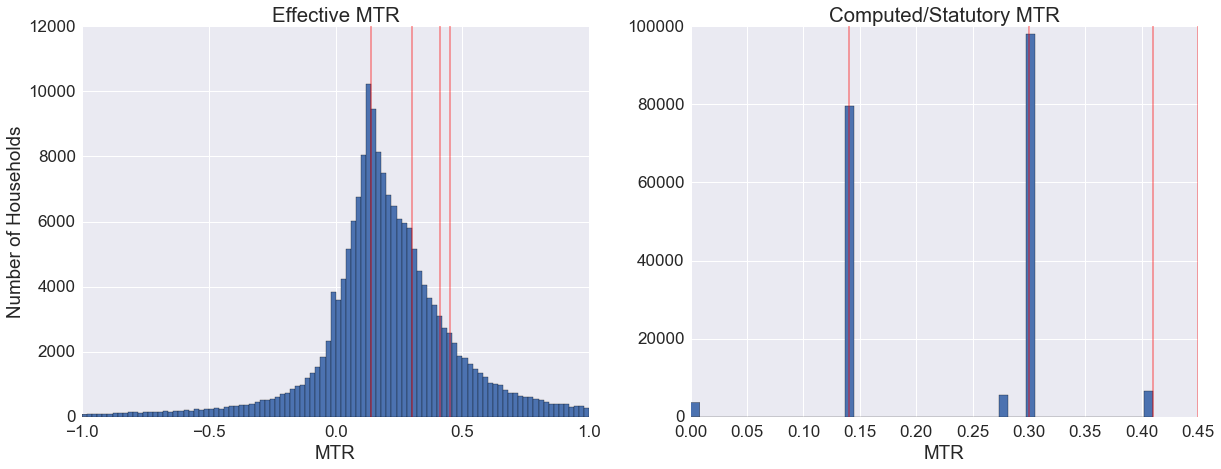
\includegraphics[width=1.2\textwidth]{/fig_casd/Effective_MTR.png}}%
% \end{figure}
% \autoref{fig:effective_statutory_rate} shows the effective MTR on the left and statutory rate on the right. 
% The effective marginal tax rate is computed by taking the difference in the tax paid in 2014 and in 2012 divided by the change in taxable income over the same period.
% \footnote{$MTR = \frac{\Delta T}{\Delta y} $}
%  Interestingly enough, I see that the distribution of an effective marginal tax rate is not a plurimodal distribution where each mode would be a mass at a given statutory MTR. In the case that households would not have changed their income such that they remain in the same tax bracket, I would have observed the distribution on the right distribution of \autoref{fig:effective_statutory_rate} which represent a probability mass function.
%  \footnote{These MTR has been computed with the tax formulas taken in Openfisca by computing the tax with \autoref{eq:variation_rate} for an $\epsilon$ of 10 euros.}



% The effective marginal tax rate distribution is not a probability mass function for two reasons, first households change or tax brackets from one year to another, and thus their MTR is a weighted average rate of the different MTR between the 2011 statutory rate and the 2014 statutory rate. Second households use tax credit and reductions. Tax credit and reductions explain that some households have a negative effective MTR: if a household that has an increase in taxable income, start to claim a tax credit such that the final tax liability is smaller despite the increase in taxable income, the effective MTR will appear to be negative.

% But what I am interested in this article is the variation in the tax base with respect to a tax reform that will be applied to the piecewise linear tax scheme. Even though the reform may imply behavioral reaction by increasing the usage of tax credits, in the absence of transaction cost to claim those tax credit, microeconomic theory state that it should not be so.

% Namely, I have

% \begin{equation*}
%   T_i(y_i,s_i) = \underbrace{t\left(\frac{y_i}{s_i}\right) \times s_i}_{\text{Observed}} - \; \underbrace{\text{tax credits}}_{\text{Unobserved}}
% \end{equation*}

% As I have very little information about tax credit and reduction in the database \footnote{it is not precisely documented, and subtracting the tax credits and reductions to the computed tax scheme do not lead to a better match between the computed income tax and the actual tax liability.}
% Tax credits lead to overestimating the tax liability of a household.




% \begin{figure}[H]
%     \centering
%     \caption{Income tax matching}
%  \label{fig:computed_vs_real_tax}
%     \begin{subfigure}{.5\textwidth}
%       \centering
%       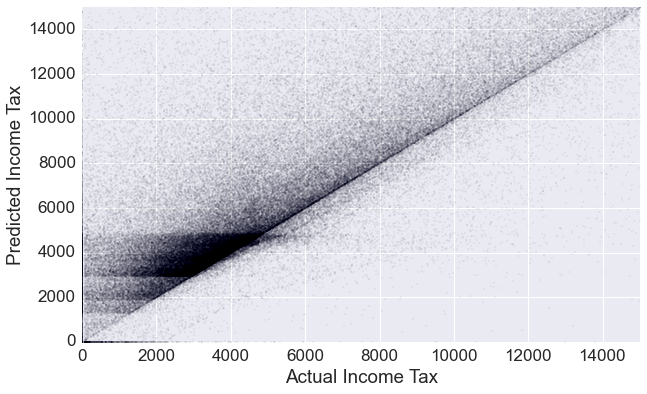
\includegraphics[width=\linewidth]{/fig_casd/zimpom_fit_2011.png}
%       \caption{Income tax 2011}
%       \label{fig:sub1}
%     \end{subfigure}%
%     \begin{subfigure}{.5\textwidth}
%       \centering
%       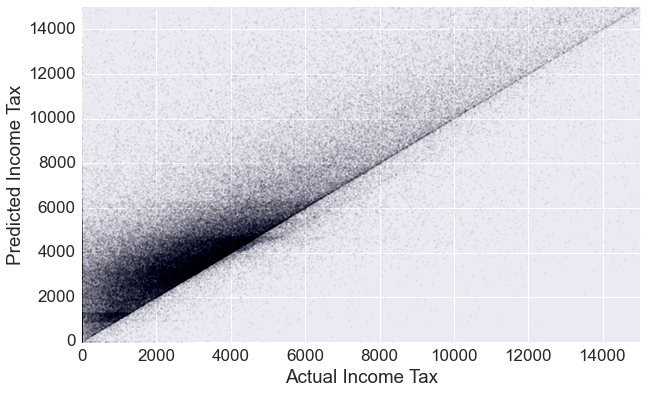
\includegraphics[width=\linewidth]{/fig_casd/zimpom_fit_2014.png}
%       \caption{Income tax 2014}
%       \label{fig:sub2}
%     \end{subfigure}
%     \label{fig:test}
% \end{figure}


% \autoref{fig:computed_vs_real_tax} shows that the computed tax is overestimated compare to actual tax liability present in the administrative database. As I see a 45 degree line that corresponds to the case where the computed income tax is equal to the actual income tax. That is the case where households do not claim any income tax credit or reduction that happened after the piecewise linear tax scheme.
% \footnote{including the family ratio scheme threshold and the decote.}


% The assumptions I make in the evaluation of the impact of the reform are: first that the households taxable income is precisely assessed, second that households would not have changed its tax bracket in the absence of the reform. As I know that these two statement is false I can still evaluate how false it is.
% %TODO: talk about same proportion going above or under due to mean reversion

% If I make the assumption that the use of tax credit is perpendicular to the tax reform, I can predict the change in tax liability by the fact that a household has been impacted or not by the reform with a regression close to the triple diff estimation.
% Indeed, I know that households treated by treatment 1 faced a change in their MTR from 14\% to the MTR they would have had in the absence of children in the household which is of 30\% for households with less than 4 children. Then I have to add the difference between the two MTR (16\% here) times the distance from the beginning of the new tax bracket (the 2014 threshold, e.g. 79,166 euros for a family of 3 children), which gives the lump sum loss that households that were between the two thresholds had.

% Thus the change in their tax liability would be:
% \[\Delta T = 0.3 \times \Delta y\ + \text{Lump sum loss for a given position between the thresholds} \]

% Households that were were impacted by the treatment 2 faced a lump sum increase of the tax equal to 836 euros times the number of fiscal shares. Thus their change in tax liability if in the 30\% tax bracket would be:


% \[\Delta T = 0.3 \times \Delta y\ + 836 \times \text{fiscal shares} \]


% I can thus estimate the change in tax liability with the following specification:

%   \begin{align}
%         \Delta T =
%         &\underbrace{
%                     \sum_{i = 1}^{6} \beta^{O}_{i} child_i \times Over_i}_
%                         {\substack{\text{Lump sum increase}\\ \text{for Treated 2 group}}}
%         + \underbrace{
%                     \sum_{i=1}^{6} \beta^{MTR_O}_i \Delta y \times child_i \times Over_i}_
%                         {\substack{\text{Average MTR for Treatment 2} \\ \text{(same as before the reform)}}}  \label{line:1} \\ 
%         &+ \underbrace{
%                     \sum_{i=1}^{6} \beta^{MTR_B}_i \Delta y \times child_i \times Between_i}_
%                         {\substack{\text{MTR of Treated group 1} \\ \text{after the reform}}}
%         + \underbrace{
%                     \sum_{i=1}^{6} \beta^{B}_i  child_i \times Between_i}_
%                         {\substack{\text{Lump sum loss of group 1} \\ \text{after the reform}}} \label{line:2}\\               
%         &+ \underbrace{
%                     \sum_{i=1}^{6} \theta_i \text{Not touched by reform}\times child_i}_
%                         {\substack{\text{Average increase in tax}\\ \text{for the untreated group}}}  
%         + \underbrace{
%                     \sum_{i=1}^{6} \gamma_i \Delta y \times \text{ Not touched by reform}\times child_i}_
%                         {\substack{\text{Average MTR by child rank}\\ \text{for the untreated group}}} \label{line:3} \\
%         &+ \epsilon_i
%   \end{align}

%   Where line (\ref{line:1}) concerns household over the 2011 thresholds. $\beta^{O}_{i}$ measures the lump sum loss for each child range that should be equal to respectively 836, 1672, 3344, 5016 6688 and 8360 for households of respectively 1 to 6 children. $\beta^{MTR_O}_i $  the average MTR for each child rank that was in treatment 2. 

%   Line (\ref{line:2}) concerns households have their 2011 taxable income between 2014 and 2011 thresholds (Treatment 1). $\beta^{MTR_B}_i$ captures the marginal tax rate of these households, it should be of 30\% for households from 1 to 4 children
%   \footnote{(and a bit more for 5 and 6 children, since some households between the thresholds, jump directly on the 41 MTR.}. $\beta^{B}_i$ captures the average lump sum loss for each rank of children, it should be equal to the weighted average difference between the 2011 tax and the 2014 tax when computed with the 2011 taxable income and should thus be lower than 836 $\times$ n euros.

  
% Line (ref{line:3}) those not impacted by the reform. $\theta$ account lump sum change in tax for households not touched by the reform which should be equal to zero if households did not change of MTR bracket which should be equal to zero. But since taxable income is on average increase over the period, it would be positive. To remedy that I include $\gamma$ to the regression that captures the average MTR in the non treated group. Since the non treated group are quite heterogeneous in terms of MTR, I include an heterogeneous effect for each child rank.
  
   

% \begin{table}[H]
% \center
% \caption{Change in tax liability}
% \label{tab: change in tax liability}
% \adjustbox{max height=\dimexpr\textheight-4.5cm\relax,
%            max width=\textwidth}{
% \begin{tabular}{lccccccccccccccccccccc}
% \toprule                         
%                                                          &    All             &    NTCI              & $\Delta y >0$         &      $\Delta y<0$ & Expected                   \\              
% $child_i \times Over_1$                                  &   1224***          &   1138***            &   908***              &   907***          &  836                       \\              
% $child_i \times Over_2$                                  &   1987***          &   1859***            &   1525***             &   1727***         &  1672                      \\              
% $child_i \times Over_3$                                  &   3682***          &   3184***            &   2970***             &   2827***         &  3344                      \\              
% $child_i \times Over_4$                                  &   5204***          &   5119***            &   4797***             &   5634***         &  5016                      \\              
% $child_i \times Over_5$                                  &   13121***         &   6920***            &   7628***             &   7602*           &  6688                      \\              
% $child_i \times Over_6$                                  &   5967***          &   6154***            &   --                  &   --              &  8360                      \\
% \midrule              
% $\Delta y \times child_i \times Over_1$                  &   0.259***         &   0.249***           &   0.267***            &   0.224***        &  $>0.3$                    \\              
% $\Delta y \times child_i \times Over_2$                  &   0.279***         &   0.275***           &   0.296***            &   0.254***        &  $>0.3$                    \\              
% $\Delta y \times child_i \times Over_3$                  &   0.310***         &   0.305***           &   0.316***            &   0.280***        &  $>0.3$                    \\              
% $\Delta y \times child_i \times Over_4$                  &   0.325***         &   0.328***           &   0.338***            &   0.343***        &  $>0.3$                    \\              
% $\Delta y \times child_i \times Over_5$                  &   0.335***         &   0.404***           &   0.378***            &   0.462**         &  $>0.3$                    \\              
% $\Delta y \times child_i \times Over_6$                  &   0.366***         &   0.389***           &   0.573***            &   0.214***        &  $>0.3$                    \\              
% $\Delta y \times child_i \times Between_1$               &   0.179***         &   0.183***           &   0.193***            &   0.128***        &  0.3                       \\              
% $\Delta y \times child_i \times Between_2$               &   0.214***         &   0.223***           &   0.258***            &   0.121***        &  0.3                       \\              
% $\Delta y \times child_i \times Between_3$               &   0.224***         &   0.230***           &   0.271***            &   0.111***        &  0.3                       \\              
% $\Delta y \times child_i \times Between_4$               &   0.236***         &   0.233***           &   0.290***            &   0.112***        &  0.3                       \\              
% $\Delta y \times child_i \times Between_5$               &   0.262***         &   0.225***           &   0.294***            &   0.111**         &  $>0.3$                    \\              
% $\Delta y \times child_i \times Between_6$               &   0.025            &   -0.019             &   -0.095              &   -0.777***       &  $>0.3$                    \\
% \midrule              
% $child_i \times Between_1$                               &   923.167***       &   910.641***         &   852.372***          &   433.385***      &  $ <836 $                  \\              
% $child_i \times Between_2$                               &   1336.725***      &   1248.149***        &   859.358***          &   590.550***      &  $ <1672$                  \\              
% $child_i \times Between_3$                               &   1963.651***      &   1783.027***        &   1189.992***         &   801.837***      &  $ <3344$                  \\              
% $child_i \times Between_4$                               &   2830.866***      &   2262.656***        &   1295.585***         &   1127.314**      &  $ <5016$                  \\              
% $child_i \times Between_5$                               &   3454.794***      &   2941.539***        &   1908.865**          &   741.941         &  $ <6688$                  \\              
% $child_i \times Between_6$                               &   3446.676***      &   10059.622***       &   12934.249           &   -17583.224***   &  $ <8360$                  \\  
% \midrule            
% Not_touched_by_reform $\times child_0$                   &   122.484***       &   109.484***         &   350.708***          &   416.135***      &   0                        \\              
% Not touched by reform $\times child_1$                   &   385.765***       &   368.151***         &   295.760***          &   299.237***      &   0                        \\              
% Not touched by reform $\times child_2$                   &   391.394***       &   268.565***         &   162.901***          &   268.073***      &   0                        \\              
% Not touched by reform $\times child_3$                   &   236.062***       &   -31.953            &   -219.547***         &   82.923          &   0                        \\              
% Not touched by reform $\times child_4$                   &   215.635**        &   -33.818            &   -199.747            &   2.925           &                            \\              
% Not touched by reform $\times child_5$                   &   253.683          &   -567.608           &   -1040.817*          &   64.932          &                            \\              
% Not touched by reform $\times child_6$                   &   194.868          &   1096.854           &   1868.347*           &   -0.000          &                            \\
% \midrule              
% $\Delta y \times$ Not touched by reform$\times child_0$  &   0.199***         &   0.183***           &   0.164***            &   0.216***        &   $>0.3$                   \\              
% $\Delta y \times$ Not touched by reform$\times child_1$  &   0.131***         &   0.128***           &   0.134***            &   0.102***        &   $>0.14$                  \\              
% $\Delta y \times$ Not touched by reform$\times child_2$  &   0.139***         &   0.148***           &   0.157***            &   0.110***        &   $>0.14$                  \\              
% $\Delta y \times$ Not touched by reform$\times child_3$  &   0.120***         &   0.156***           &   0.170***            &   0.096***        &   $>0.14$                  \\              
% $\Delta y \times$ Not touched by reform$\times child_4$  &   0.093***         &   0.141***           &   0.150***            &   0.085           &   $>0.14$                  \\              
% $\Delta y \times$ Not touched by reform$\times child_5$  &   0.075***         &   0.157***           &   0.177***            &   0.135           &   $>0.14$                  \\              
% $\Delta y \times$ Not touched by reform$\times child_6$  &   0.112***         &   0.046              &   0.002               &   0.844           &   $>0.14$                  \\ 
% \midrule \bottomrule             
% adjusted-R2                                              &   40.15\%          &   62.82\%            &   57.39\%             &   47.19\%         &                             \\              
% N                                                        &   193555           &   87773              &   69144               &   18629           &                            \\                
% \bottomrule
% \end{tabular}
% }
% \end{table}                         


% The first column represents the above equation on the total population. I see that I do not perfectly structurally match the tax reform,  but that the order of magnitude is quite consistent from 1 to 4 children. 
% \footnote{
% For 5 and 6 children, it is not the case. The number of observation (respectively 42 and 5) will make it very dependent to outliers, regressions with iteratively reweighted least squares lower significantly the figures for 5 children)}
% The impact of the lump sum increases are overestimated, but I see that the MTR of treated 2 groups are underestimated up to 2 children. Once the constant for each group is correctly assessed, I see that the lump sum increase in tax is pretty well assessed.




% \subsection{Extensive margin:}





% \section{Threats to identification}

% \subsection{Mean Reversion and Change in the distribution bias}
% Change in the distribution bias: control for position in the income distribution. 
% Mean reversion: Interestingly the income position where the tax reforms happens is not (as a lot of other analyed tax reform) at the top of the income distribution. 

% \subsection{Underestimating the Tax-Base}
% There exist a tax-break applying to the labor income tax base. By default, total labor income face a 10\% tax exemption. In the case that the tax-payer has professional expenses that are higher than the 10\% tax exemption, she may choose to switch from the default tax exemption to the so called \emph{real expenses} \footnote{"Aux frais réels" in French}.
% More on it (deductions pour trajets, les plus riches y recourent plus, etc)
% \paragraph{Consequences:}
% The consequence in that for a significant share of households, the tax-base has a measurment error that leads it to be underestimated. Meaning that households that where exected to be in the Treatment 1 where is fact not treated.
% 3 possible cases exists:
% \begin{enumerate}
%   \item The household is in the treatment 1 group although it was not treated $\implies$, it would thus under-estimates the effect since a treated group will be composed of non-treated households.
%   \item  The household is in the treatment 2 group although it was in the treatment 1 group $\implies$, it would (depend of the effect ?) aply 
% \end{enumerate}





% \subsection{Common trend assumption}

% \subsection{The change of tax base for capital income}
% Control ZIMPVALM_2011
% \subsection{Retirement pensions tax reforms}


% \newpage



\paragraph{Double Differences:} As the reform embodies a triple diff in its inner nature, it might not be obvious what a double diff could be. It could be for each child rank to compare what happened above or below thresholds. It could be to run a regression on a specific treated group with households without children in the same position of the income distribution as the reference group. 


Another solution would be to implement a simple DD with two treatments as in \autoref{eq:DD_simple}. This is what is done in the first (1) regression of \autoref{table:DD}  where I regress the tax reform would have impacted the change in taxable income between 2011 and 2014 based on whether or not a household if its income did not change. This shows that the reform had a negative impact on both households that face a change in MTR and a lump sum decrease. The interpretation would be that the substitution effect dominates for households that face an increase in their MTR (Treatment 1). Households that face a lump sum decrease in their disposable income would have reacted by decreasing their taxable income. This last interpretation would not be consistent with microeconomic theory as it would imply that households utility is decreasing either in income or in leisure.
\footnote{Marginal rate of substitution supposes that taxpayers are willing to trade one unit of leisure for n of disposable income. If households increase their leisure when their disposable income decreases, it implies that the sign of n is negative and thus that either leisure or disposable income is (at least locally) a bad}
However, that regression is biased since it does not take into account trends that could be specific to change a specific location in the income distribution.


 I can look at column (2) once I controlled for the income location. 





\begin{table}[H]
\center
\caption{Double Differences with different types of controls}
\label{table:DD}
\adjustbox{max height=\dimexpr\textheight-4.5cm\relax,
           max width=\textwidth}{
\begin{tabular}{lcccc}
\toprule
                                        &  (1)  &  (2) & (3) & (4)        \\      
\midrule
Treatment 1                             & -1342***      & 3990***       & -3033***      & 2490***                \\   
                                        & (107)         & (139)         & (107)         & (147)                  \\   
Treatment 2                             & -1472***      & 4148***       & -2883***      & 3313***                \\ 
                                        & (105)         & (169)         & (108)         & (192)                  \\   
\midrule  
Intercept                               & 6647***       & 8625     ***  & 3113***       & 6335***                \\   
                                        & (37)          & (40)          & (79)          & (83)                   \\  
\midrule 
Taxable income $\in$ $[58291,63233]$    &               & -5973***      &               & -5707***               \\   
                                        &               & (100)         &               & (99)                   \\   
Taxable income $\in$ $[63233,63530]$    &               & -6020***      &               & -5977***               \\   
                                        &               & (390)         &               & (382)                  \\   
Taxable income $\in$ $[63530,73516]$    &               & -7439***      &               & -6738***               \\   
                                        &               & (125)         &               & (129)                  \\   
Taxable income $\in$ $[73516,73806]$    &               & -7815***      &               & -7480***               \\   
                                        &               & (637)         &               & (632)                  \\   
Taxable income $\in$ $[73806,84103]$    &               & -7717***      &               & -7129***               \\   
                                        &               & (178)         &               & (189)                  \\   
Taxable income $\in$ $[84103,94368]$    &               & -8120***      &               & -7574***               \\   
                                        &               & (221)         &               & (231)                  \\   
Taxable income $\in$ $[94368,94451]$    &               & -8230***      &               & -7723***               \\   
                                        &               & (1848)        &               & (1856)                 \\   
Taxable income $\in$ $[94451,104633]$   &               & -7300***      &               & -6942***               \\   
                                        &               & (282)         &               & (292)                  \\   
Taxable income $\in$ $[104633,115185]$  &               & -7530***      &               & -7187***               \\   
                                        &               & (347)         &               & (355)                  \\   
Taxable income $\in$ $[115185,135941]$  &               & -7380***      &               & -7170***               \\   
                                        &               & (338)         &               & (348)                  \\   
Taxable income $\in$ $[135941,150684]$  &               & -6290***      &               & -6110***               \\   
                                        &               & (524)         &               & (529)                  \\   
Taxable income over 150684 euros        &               & -8273***      &               & -8167***               \\   
                                        &               & (473)         &               & (481)                  \\
\midrule   
1 child1                                &               &               & 4135***       & 1244***               \\     
                                        &               &               & (117)         & (124)                    \\   
2 child2                                &               &               & 5073***       & 2898***               \\     
                                        &               &               & (94)          & (94)                     \\   
3 child3                                &               &               & 6021***       & 4715***               \\     
                                        &               &               & (116)         & (112)                    \\   
4 child4                                &               &               & 6948***       & 6189***               \\     
                                        &               &               & (253)         & (249)                    \\   
5 child5                                &               &               & 6658***       & 6432***               \\     
                                        &               &               & (674)         & (672)                    \\   
6 child6                                &               &               & 7216***       & 7626***               \\   
                                        &               &               & (1364)        & (1362)                 \\   
\bottomrule
Number of observations & 193555 & 193555 & 193555 &  193555 \\
\bottomrule
\end{tabular}
}
\end{table}

As the mean increase in the population is of 8625 euros, I see that being on a specific location of the income distribution has a negative effect. As an example, the marginal impact of earning between 84103 and 94368 euros in 2011 is a decrease in declared taxable income of 8230 euros in 2014 compared to households earning less than 58291 euros. Treatments have both a positive impact on the change in the tax base, households when controlling only for the position in the income distribution. Wich would mean that the income effect strongly dominates the substitution effect. However, when controlling just for the number of children (3), the effect is strongly negative with a decrease in taxable income of about 3000 euros for both treated group. 

When controlling for both income position and the number of children (4), both difference in trends for the number of children, the impact of each treatment is positive. Meaning that I indeed observe a pure positive income effect (Treatment 2), and a substitution effect that the dominates the income effect (Treatment 1). However, I can note that regression (4) is just a pooled triple-diff, namely the weighted average of the triple diff. 

\section{Loss in precentage of disposable income.}  
 \begin{figure}[H]
    \caption{Loss in relative disposable income due to the reform.}
 \label{fig:percent_loss}
  \makebox[\textwidth][c]{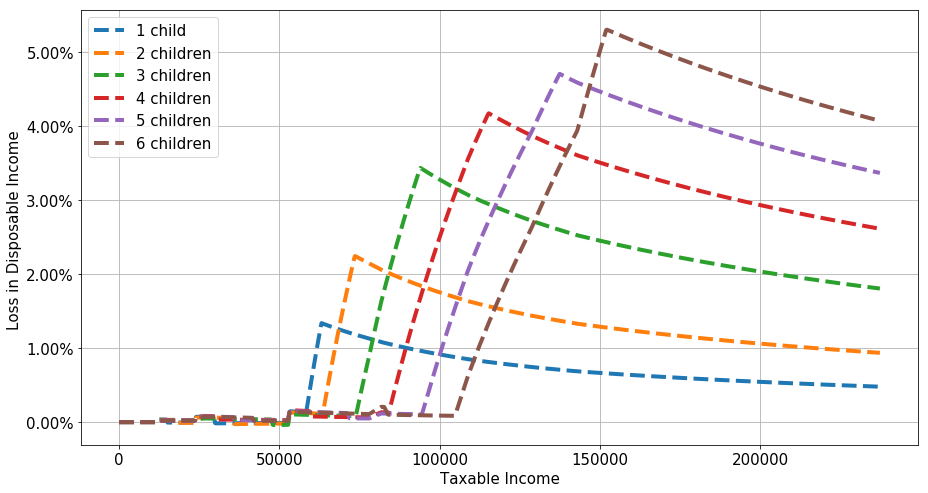
\includegraphics[width=1.2\textwidth]{loss_in_relative_disposable_income.png}}%
  %\label{fig:MTR_single_couple}
\end{figure}

\section{Extensive margins, probability linear models:}
\vspace{-5cm}
\let\cleardoublepage\clearpage
\newgeometry{top=1mm, bottom=1mm, left = 7mm, right =  1mm} 
\afterpage{
\begin{landscape}
\pagestyle{plain}
\begin{table}[H]
\center
\adjustbox{max height=19.5cm,
           max width= 22 cm}{
\begin{tabular}{lccccccccccccccccccccc}
\toprule 
                                                  & Me_start_working        &     Wo_start_working       &   Me_stop_working_not_retired  &  Wo_stop_working_not_retired &                   Me_get_retired &       Wo_get_retired                       \\
                                                  \cmidrule(lr){2-2}  \cmidrule(lr){3-3} \cmidrule(lr){4-4} \cmidrule(lr){5-5}  \cmidrule(lr){6-6} \cmidrule(lr){7-7}
$Over_{1} \times Child_1$                         & 0.0032**                &     0.0058***              &   -0.0256***                   &  0.0001                      &                   -0.0196***     &       -0.0092***                           \\
                                                  & (0.0015)                &     (0.0017)               &   (0.0057)                     &  (0.0038)                    &                   (0.0034)       &       (0.0027)                             \\
$Over_{1} \times Child_2$                         & 0.0086***               &     0.0010                 &   -0.0480***                   &  0.0007                      &                   -0.0290***     &       -0.0090***                           \\
                                                  & (0.0012)                &     (0.0016)               &   (0.0050)                     &  (0.0033)                    &                   (0.0034)       &       (0.0029)                             \\
$Over_{1} \times Child_3$                         & 0.0064***               &     -0.0147***             &   -0.0519***                   &  0.0057                      &                   -0.0256***     &       -0.0065**                            \\
                                                  & (0.0015)                &     (0.0026)               &   (0.0067)                     &  (0.0046)                    &                   (0.0036)       &       (0.0031)                             \\
$Over_{1} \times Child_4$                         & 0.0017                  &     -0.0206**              &   -0.0602***                   &  0.0140                      &                   -0.0239***     &       -0.0019                              \\
                                                  & (0.0034)                &     (0.0082)               &   (0.0149)                     &  (0.0110)                    &                   (0.0042)       &       (0.0047)                             \\
\midrule
$Between1 \times Child_1$                         & 0.0013                  &     0.0085***              &   -0.0093                      &  0.0011                      &                   -0.0016        &       -0.0012                              \\
                                                  & (0.0018)                &     (0.0023)               &   (0.0078)                     &  (0.0056)                    &                   (0.0037)       &       (0.0027)                             \\
$Between1 \times Child_2$                         & 0.0065***               &     0.0040**               &   -0.0113**                    &  0.0047                      &                   -0.0214***     &       -0.0067***                           \\
                                                  & (0.0012)                &     (0.0017)               &   (0.0051)                     &  (0.0036)                    &                   (0.0028)       &       (0.0023)                             \\
$Between1 \times Child_3$                         & 0.0047***               &     -0.0054*               &   -0.0286***                   &  -0.0032                     &                   -0.0258***     &       -0.0096***                           \\
                                                  & (0.0016)                &     (0.0028)               &   (0.0067)                     &  (0.0045)                    &                   (0.0035)       &       (0.0029)                             \\
$Between1 \times Child_4$                         & 0.0017                  &     -0.0168**              &   -0.0382***                   &  -0.0017                     &                   -0.0256***     &       -0.0067*                             \\
                                                  & (0.0036)                &     (0.0079)               &   (0.0138)                     &  (0.0091)                    &                   (0.0043)       &       (0.0039)                             \\
\midrule                                                  
$Child_1$                                         & -0.0019                 &     -0.0011                &   0.0808***                    &  -0.0052*                    &                   -0.0338***     &       -0.0260***                           \\
$Child_2$                                         & -0.0053***              &     0.0064***              &   0.0629***                    &  -0.0189***                  &                   -0.0301***     &       -0.0184***                           \\
$Child_3$                                         & -0.0020                 &     0.0250***              &   0.0529***                    &  -0.0257***                  &                   -0.0344***     &       -0.0180***                           \\
$Child_4$                                         & 0.0030                  &     0.0462***              &   0.0388***                    &  -0.0264***                  &                   -0.0377***     &       -0.0186***                           \\
\midrule
Taxable income $\in$ $[58291,63233]$              & -0.0090***              &     -0.0140***             &   0.0209***                    &  0.0085***                   &                   -0.0005        &       -0.0018                              \\
Taxable income $\in$ $[63233,63530]$              & -0.0067**               &     -0.0137***             &   0.0312***                    &  0.0165**                    &                   -0.0040        &       -0.0059                              \\
Taxable income $\in$ $[63530,73516]$              & -0.0120***              &     -0.0153***             &   0.0374***                    &  0.0071***                   &                   0.0149***      &       0.0021                               \\
Taxable income $\in$ $[73516,73806]$              & -0.0147***              &     -0.0166***             &   0.0604***                    &  0.0071                      &                   0.0165**       &       -0.0012                              \\
Taxable income $\in$ $[73806,84103]$              & -0.0128***              &     -0.0126***             &   0.0684***                    &  0.0092***                   &                   0.0210***      &       0.0040                               \\
Taxable income $\in$ $[84103,94368]$              & -0.0118***              &     -0.0101***             &   0.0838***                    &  0.0108***                   &                   0.0196***      &       0.0026                               \\
Taxable income $\in$ $[94368,94451]$              & -0.0182***              &     -0.0248***             &   0.0869**                     &  -0.0314                     &                   0.0033         &       -0.0145***                           \\
Taxable income $\in$ $[94451,104633]$             & -0.0135***              &     -0.0044**              &   0.0947***                    &  0.0012                      &                   0.0214***      &       0.0031                               \\
Taxable income $\in$ $[104633,115185]$            & -0.0151***              &     -0.0065***             &   0.1084***                    &  0.0064                      &                   0.0179***      &       0.0018                               \\
Taxable income $\in$ $[115185,135941]$            & -0.0144***              &     -0.0074***             &   0.1185***                    &  0.0091**                    &                   0.0136***      &       -0.0034                              \\
Taxable income $\in$ $[135941,150684]$            & -0.0147***              &     -0.0057**              &   0.1406***                    &  0.0067                      &                   0.0104**       &       -0.0026                              \\
Taxable income over 150684 euros                  & -0.0170***              &     -0.0052**              &   0.1605***                    &  0.0125**                    &                   0.0067         &       -0.0020                              \\
\midrule
Intercept                                         & 0.0877***               &     0.1316***              &   -1.1587***                   &  -0.0323**                   &                   0.3897***      &       0.3532***                            \\
\midrule
Age_wo                                            & 0.0012***               &     -0.0058***             &   0.0063***                    &  0.0070***                   &                   -0.0017***     &       -0.0118***                           \\
                                                  & (0.0003)                &     (0.0007)               &   (0.0012)                     &  (0.0004)                    &                   (0.0006)       &       (0.0005)                             \\
Age_me                                            & -0.0046***              &     0.0012**               &   0.0959***                    &  0.0002                      &                   -0.0186***     &       -0.0066***                           \\
                                                  & (0.0006)                &     (0.0005)               &   (0.0018)                     &  (0.0007)                    &                   (0.0008)       &       (0.0006)                             \\
I(Age_wo_squared / 10 ** 4)                       & -0.1025***              &     0.5614***              &   -1.1955***                   &  -0.9674***                  &                   0.2693***      &       1.7518***                            \\
                                                  & (0.0348)                &     (0.0721)               &   (0.1369)                     &  (0.0527)                    &                   (0.0713)       &       (0.0650)                             \\
I(Age_me_squared / 10 ** 4)                       & 0.5090***               &     -0.1009**              &   -11.8298***                  &  -0.0203                     &                   2.5521***      &       0.7521***                            \\
                                                  & (0.0653)                &     (0.0477)               &   (0.1955)                     &  (0.0747)                    &                   (0.0865)       &       (0.0708)                             \\
I(Age_Elder_child / 10 ** 4)                      & 0.9410**                &     -1.4765**              &   -0.9211                      &  -13.8524***                 &                   -2.3328***     &       -0.8657                              \\
                                                  & (0.4754)                &     (0.6009)               &   (1.8390)                     &  (1.2051)                    &                   (0.8539)       &       (0.6875)                             \\
\hdrule
\midrule
adjusted-R2                                       & 0.54\%                  &     0.94\%                 &   26.85\%                     &  0.44\%                       &                   11.72\%        &       9.43\%                                \\
N                                                 & 192640                  &     192640                 &   192640                       &  192640                      &                   192640         &       192640                               \\
\bottomrule
\end{tabular}
}
\end{table} 

\end{landscape}
}
\end{subappendices}
\restoregeometry 
\addcontentsline{toc}{section}{References}
\bibliography{Qf_lowering}
\newpage
  \chapter*{Conclusion}
  \addcontentsline{toc}{chapter}{Conclusion}
Cette thèse a visée à ouvrir des pistes d'amélioration des politiques publiques. Le premier en explorant un détail technique, la temporalité de l'impôt, relativement inexploré par la littérature. Le second en documentant des comportements de non-optimisation de la part des ménages documente de nouveaux comportements vis à vis d'un système fiscal lié a des choix d'optimisation lors de la déclaration fiscale. Le troisième en essayant d'identifier via une nouvelle méthodologie le comportement des ménages aisés vis à vis des modifications de l'impôt, tout en identifiant séparément les effets revenus des effets de substitution.

%\bibliographystyle{plain}
%\addcontentsline{toc}{chapter}{Bibliography}
%\bibliography{monthly_income_tax_frequency}




%%%%%%%%%%%%%%%%%%%%%%%%%%%%%%%%%%%%%%%%%%%%%%%%%%%%%%%%%%%%%%%%%%%%%%%%%%%%%%%%%%%%%%%%%%%%%%%%%%%%%%%%%%%%%%


\ifx\isEmbedded\undefined
\newpage
%\bibliography{tax_frequency}
\end{document}
\else \fi